\documentclass[a4paper,11pt,twoside]{report}

\usepackage[left=2.5cm,right=2cm,top=2cm,bottom=2cm]{geometry}

\usepackage[utf8]{inputenc}

\usepackage[T1]{fontenc}
\usepackage{lmodern}
\usepackage{amssymb}

%\usepackage{graphicx}
\usepackage{prooftree,amsmath,wasysym,xcolor,xspace}
\ifx\pdftexversion\undefined
\usepackage[dvips]{graphicx}
\else
\usepackage{graphicx}
\DeclareGraphicsRule{*}{mps}{*}{}
\fi
\usepackage{mathptmx}
\usepackage{stmaryrd}
\usepackage{eurosym}
\usepackage{amsbsy}
\usepackage{latexsym}
\usepackage{url}
\usepackage{suffix}
\usepackage{listings}
\usepackage{color}
\usepackage{verbatim}
\usepackage{citesort}
\usepackage{tikz}
\usepackage{pslatex}
\usepackage{comment}
\usepackage{times}
%\usepackage{space}
\usepackage{etex}
\usepackage{epstopdf}
%\usepackage{microtype}  % Looks better but may take more space (only works for pdflatex)
\usepackage[all]{xypic}

\newcommand{\upd}{\mathit{update}}
\newcommand{\pn}{\p}
\newcommand{\rtsyntax}[1]{\colorbox{lightgray}{\ensuremath{#1}}}
\newcommand{\ptilde}[1]{{\ensuremath{#1}}}
%\newcommand{\kf}[1]{\textsf{\upshape\small #1}\xspace}
\newcommand{\kf}[1]{\textup{\textsf{#1}}\xspace}
\newcommand{\constf}[1]{\textup{\textsf{#1}}}
\newcommand{\srsimple}[3]{\ensuremath{\bar{#1}[#2](#3)}}
\newcommand{\sr}[4]{\ensuremath{\srsimple{#1}{#2}{#3}.#4}}
\newcommand{\uu}{\ensuremath{u}}
\newcommand{\Ia}{\ensuremath{a}}
\newcommand{\Ic}{\ensuremath{c}}
\newcommand{\Iu}{\ensuremath{u}}
\newcommand{\Ik}{\ensuremath{k}}
\newcommand{\Ias}{\ensuremath{\alpha}}
\newcommand{\Ib}{\ensuremath{b}}
\newcommand{\y}{\ensuremath{y}}
\newcommand{\PP}{\ensuremath{P}}
\newcommand{\Q}{\ensuremath{Q}}
\newcommand{\R}{\ensuremath{R}}
\newcommand{\DD}{\ensuremath{D}}
\newcommand{\sasimple}[3]{\ensuremath{#1[#2](#3)}}
\newcommand{\sa}[4]{\ensuremath{\sasimple{#1}{#2}{#3}.#4}}
\newcommand{\pp}{\ensuremath{\at{\p}}}
\newcommand{\si}[2]{\ensuremath{#1[#2]}}
\newcommand{\sI}[1]{\ensuremath{\s_{#1}}}
%\newcommand{\sI}[1]{\ensuremath{\s^#1}}   vecchia versione
\newcommand{\sii}{\si{\s}{\p}}
\newcommand{\sij}{\si{\s}{\p_j}}
\newcommand{\siq}{\si{\s}{\q}}
\newcommand{\siip}{\si{\s'}{\p'}}
\newcommand{\sipp}{\si{\s'}{\p}}
\newcommand{\cc}{\ensuremath{c}}
\newcommand{\pset}{\ensuremath{\Pi}}
\newcommand{\inpset}[2][\Pi]{\ensuremath{\p_#2 \in #1}}
\newcommand{\kinpset}{\inpset{k}}
%\newcommand{\pset}{\ensuremath{\set{\participant{\p}_k}_{k\in K}}}
\newcommand{\out}[4]{\ensuremath{#1!\langle \pset,#2\rangle;#4}}
%\newcommand{\out}[4]{\ensuremath{#1!\langle \set{#3_k}_{k\in K},#2\rangle;#4}}
\newcommand{\outp}[3]{\ensuremath{#1!\langle \pset,#2\rangle}}
\newcommand{\outs}[4]{\ensuremath{#1!\langle #3,#2\rangle;#4}}
\newcommand{\e}{\ensuremath{e}}
\newcommand{\inp}[4]{\ensuremath{#1?( #3,#2);#4}}
\newcommand{\inpp}[3]{\ensuremath{#1?( #3,#2)}}
\newcommand{\inps}[4]{\ensuremath{#1?( #3,#2);#4}}
\newcommand{\x}{\ensuremath{x}}
\newcommand{\participant}[1]{\ensuremath{\mathtt{#1}}}
\newcommand{\q}{\ensuremath{\participant{q}}}
\newcommand{\p}{\ensuremath{\participant{p}}}
\newcommand{\sd}[4]{\ensuremath{#1!\langle\! \langle#3,#2\rangle \!\rangle;#4}}
\newcommand{\sdt}[4]{\ensuremath{#1^\top!\langle\! \langle#3,#2\rangle \!\rangle;#4}}
\newcommand{\sdp}[4]{\ensuremath{#1!^{\lev'}\langle\! \langle#3,#2\rangle \!\rangle.#4}}
\newcommand{\rd}[4]{\ensuremath{#1?(\!(#3,#2)\!);#4}}
\newcommand{\rdt}[4]{\ensuremath{#1^\top?(\!(#3,#2)\!).#4}}
\newcommand{\z}{\ensuremath{z}}
\newcommand{\pc}{\Par}
\newcommand{\s}{\ensuremath{s}}
\newcommand{\X}{\ensuremath{X}}
\newcommand{\defX}{\ensuremath{\kf{def} \ \Ddef\ \kf{in}\ }}
\newcommand{\Xsignature}{\ensuremath{\X(\at{x}, \at{y})}}
\newcommand{\Ddef}{\ensuremath{\Xsignature=\PP}}
\newcommand{\Ddefp}{\ensuremath{\Xsignature=\PP'}}
\newcommand{\defIn}[1]{\ensuremath{\kf{def} \ #1 \ \kf{in}\ }}
\newcommand{\defD}{\ensuremath{\kf{def}\ \DD \ \kf{in}\ }}
\newcommand{\DdefD}{\ensuremath{\kf{def}\ \Ddef \ \kf{in}\ }}
\newcommand{\defDp}{\ensuremath{\kf{def}\ \DD' \ \kf{in}\ }}
\newcommand{\proccall}[3]{\ensuremath{#1\langle\ptilde{#2},\ptilde{#3}\rangle}}
\newcommand{\proccallw}[3]{\ensuremath{#1\langle\ptilde{#2},\ptilde{#3}\rangle}}
\newcommand{\proccalldots}[3]{\ensuremath{#1\langle\ptilde{#2},\ptilde{#3}\rangle}}

\newcommand{\indexed}[4]{\ensuremath{\{#1_#3 : #2_#3\}_{#3 \in #4}}}

\newcommand{\values}{\ensuremath{\at{v}}}
\newcommand{\trival}[3]{\ensuremath{(#3,#2, #1)}}
\newcommand{\labval}[2]{\ensuremath{(#1, #2)}}
\newcommand{\anglep}[2]{\ensuremath{\langle #1, #2\rangle}}
\newcommand{\valheap}[3]{\ensuremath{( #3,\pset,#1 )}}
\newcommand{\valheaps}[3]{\ensuremath{( #3,#2,#1 )}}
\newcommand{\valheapj}[2]{\ensuremath{( #2,\{j\},#1 )}}
\newcommand{\valheapp}[2]{\ensuremath{( #2,\{\p\},#1 )}}
\newcommand{\valheapLess}[3]{\ensuremath{( #3,\pset\setminus \p,#1 )}}
\newcommand{\delheap}[3]{\ensuremath{(#3,{#2},#1 )}}
\newcommand{\labheap}[3]{\ensuremath{( #3,\pset,#1 )}}
\newcommand{\labheaps}[3]{\ensuremath{( #3,#2,#1 )}}
\newcommand{\labheapj}[2]{\ensuremath{( #2,\{j\},#1 )}}
\newcommand{\labheapp}[2]{\ensuremath{( #2,\{\p\},#1 )}}
\newcommand{\lsel}[4]{\ensuremath{#1 \oplus \anglep{\pset}{#2};#4}}
\newcommand{\lbranch}[2]{\ensuremath{#1 \&
({#2},\indexed{l}{\PP}{i}{I})}}
\newcommand{\lbranchi}[2]{\ensuremath{#1 \&
({#2},\indexed{l}{\PP}{i}{I})}}
\newcommand{\ifthenelse}[3]{\ensuremath{\kf{if}\ #1\ \kf{then}\ #2\ \kf{else}\ #3}}
\newcommand{\ift}[2]{\ensuremath{\kf{if}\ #1\ \kf{then}\ #2}}
\newcommand{\inact}{\ensuremath{\mathbf{0}}}
\newcommand{\nuc}[2]{\ensuremath{(\nu #1)#2}}
\newcommand{\AND}[2]{\ensuremath{#1\ \kf{and}\ #2}}
\newcommand{\NOT}[1]{\ensuremath{\kf{not}\ #1}}
\newcommand{\true}{\kf{true}}
\newcommand{\false}{\kf{false}}
\newcommand{\h}{\ensuremath{h}}
\newcommand{\mg}{\ensuremath{m}}
\newcommand{\va}{\ensuremath{v}}
\newcommand{\at}[1]{\ensuremath{\ptilde{#1}}}
\newcommand{\atw}[1]{\ensuremath{\ptilde{#1}}}
\newcommand{\Co}[1]{\ensuremath{C[#1]}}
\newcommand{\Par}{\ensuremath{\ |\ }}
\newcommand{\cas}{\ensuremath{r}}
\newcommand{\eq}{\ensuremath{$\diameter$}}

%SEMANTICA
\newcommand{\redsym}{\ensuremath{\longrightarrow}}
\newcommand{\red}[2]{\ensuremath{#1\redsym#2}}
\newcommand{\redM}[2]{\ensuremath{#1\redsym^*#2}}
\newcommand{\set}[1]{\ensuremath{\{#1\}}}
\newcommand{\sub}[2]{\ensuremath{\{#1/#2\}}}
\newcommand{\ssub}[2]{\ensuremath{\{#1/#2\}}}
\newcommand{\subO}[2]{\ensuremath{\set{\!\{#1/#2\}\!}}}

\newcommand{\sep}{\ensuremath{~\mathbf{|}~ }}

\newcommand{\Implies}{\ensuremath{\quad \Rightarrow \quad }}

\newcommand{\mqueue}[2]{\ensuremath{#1 : #2}}
\newcommand{\emptyqueue}[1]{\mqueue{\s}{\emptyset}}
\newcommand{\queue}{\ensuremath{\h}}
\newcommand{\stdqueue}{\mqueue{\s}{\queue}}
\newcommand{\qcomp}[2]{\ensuremath{#1 \cdot #2}}
\newcommand{\qtail}[1]{\ensuremath{\qcomp{\queue}{#1}}}
\newcommand{\qhead}[1]{\ensuremath{\qcomp{#1}{\queue}}}

\newcommand{\qappend}[1]{\mqueue{\s}{\qtail{#1}}}
\newcommand{\qpop}[1]{\mqueue{\s}{\qhead{#1}}}

\newcommand{\subst}[2]{\ensuremath{\{#1 / #2\}}}
\newcommand{\remove}[2]{\ensuremath{#1 \backslash \{#2\}}}

\newcommand{\freen}[1]{\ensuremath{\text{fn}(#1)}}
\newcommand{\dpv}[1]{\ensuremath{\text{dpv}(#1)}}
\newcommand{\fpv}[1]{\ensuremath{\text{fpv}(#1)}}
\newcommand{\rrule}[1]{[\text{#1}]}

%TIPI
\newcommand{\G}{\ensuremath{G}}
\newcommand{\Gv}[4]{\ensuremath{#1\to\pset:\langle#3\rangle.#4}}
\newcommand{\Gvr}[4]{\ensuremath{#1\to#2:\langle#3\rangle.#4}}
\newcommand{\U}{\ensuremath{U}}
\newcommand{\sid}[1]{\ensuremath{\textup{pn}(#1)}}
\newcommand{\pro}[2]{\ensuremath{#1\upharpoonright#2}}
\newcommand{\Ga}{\ensuremath{\Gamma}}
\newcommand{\D}{\ensuremath{\Delta}}
%\newcommand{\Dp}{\ensuremath{\D'}}
\newcommand{\T}{\ensuremath{T}}
\newcommand{\TQ}{\ensuremath{{\tt{T}}}}
\newcommand{\TG}{\ensuremath{{\mathsf{T}}}}
\newcommand{\Tp}{\ensuremath{T'}}
\newcommand{\ST}{\ensuremath{S}}
\newcommand{\TT}{\atw{\T}}
\newcommand{\SST}{\atw{S}}
\newcommand{\UT}{\ensuremath{U}}
\newcommand{\oT}[2]{\ensuremath{\;!\langle #2,#1\rangle}}
\newcommand{\iT}[2]{\ensuremath{?( #2,#1 )}}
\newcommand{\oTG}[2]{\ensuremath{\;\natural\langle #2,#1\rangle}}
\newcommand{\oTGp}[2]{\ensuremath{\;\natural'\langle #2,#1\rangle}}
\newcommand{\an}[1]{\ensuremath{\langle #1\rangle}}
\newcommand{\de}[3]{\ensuremath{#1\vdash#2:#3}}
\newcommand{\der}[3]{\ensuremath{#1\vdash#2\triangleright#3}}
\newcommand{\dom}[1]{\ensuremath{dom( #1)}}
\newcommand{\range}[1]{\ensuremath{range( #1)}}
\newcommand{\ty}{\textbf{t}}
\newcommand{\End}{\kf{end}}
\newcommand{\Bool}{\kf{bool}}
\newcommand{\Nat}{\kf{nat}}
%\newcommand{\setk}[1]{\ensuremath{\set{#1_k}_{k\in K}}}

\newcommand{\SelType}[2]{\ensuremath{\oplus(#1,#2)}}

\newcommand{\seltype}{\ensuremath{\oplus \langle \pset,\{l_i:\T_i\}_{i\in
I} \rangle }}
\newcommand{\seltypeG}{\ensuremath{\oplus(\pset,\{l_i:\pro{\G_i}\q\}_{i\in I})}}
\newcommand{\seltypeT}{\ensuremath{\oplus\{l_i:\pro{\T_i}\q\}_{i\in I}}}
\newcommand{\seltypeTp}{\ensuremath{\oplus\{l_i:\T_i\}_{i\in I}}}
\newcommand{\seltypeq}{\ensuremath{\oplus\langle\pset,l\rangle;\T}}
\newcommand{\seltypeqg}{\ensuremath{\oplus\langle\pset,l\rangle;\TG}}
\newcommand{\seltypeqj}{\ensuremath{\oplus\langle\{j\},l\rangle;\T}}
\newcommand{\seltypeqq}{\ensuremath{\oplus\langle\{\q\},l\rangle;\T}}
\newcommand{\seltypep}{\ensuremath{\oplus(\pset,l);\T'}}
\newcommand{\seltypezp}{\ensuremath{\oplus(\pset,l:\T_0;\T')}}
\newcommand{\seltypez}{\ensuremath{\oplus(\pset,l:\T_0)}}
\newcommand{\seltypei}{\ensuremath{\oplus\langle\pset,l_i\rangle;\T_i}}
\newcommand{\seltypej}{\ensuremath{\oplus(\pset,l_j);\T_j}}
\newcommand{\seltypesi}{\ensuremath{\oplus(\pset,l_{i})}}
\newcommand{\seltypesip}{\ensuremath{\oplus(\pset,l_{i'})}}
\newcommand{\seltypesipz}{\ensuremath{\oplus(\pset,l_{i_0})}}
\newcommand{\seltypesipzs}{\ensuremath{\oplus(\set\p,l_{i_0})}}
\newcommand{\seltypesipjz}{\ensuremath{\oplus(\pset\setminus \p,l_{i_0})}}
\newcommand{\seltypesipj}{\ensuremath{\oplus(\pset\setminus \p,l_{i'})}}
\newcommand{\seltypes}{\ensuremath{\oplus\langle\pset,l\rangle}}
\newcommand{\seltypesem}{\ensuremath{\oplus(\emptyset,l)}}
\newcommand{\seltypesemZ}{\ensuremath{\oplus(\emptyset,Z)}}
\newcommand{\branchtype}{\ensuremath{\&(\p,\{l_i:\T_i\}_{i\in I})}}
\newcommand{\branchtypeq}{\ensuremath{\&(\q,\{l_i:\T_i\}_{i\in I})}}
\newcommand{\branchtypeG}{\ensuremath{\&(\p,\{l_i:\pro{\G_i}\q\}_{i\in I})}}
\newcommand{\branchtypeT}{\ensuremath{\&\{l_i:\pro{\T_i}\q\}_{i\in I}}}
\newcommand{\branchtypeTp}{\ensuremath{\&\{l_i:\T'_i\}_{i\in I}}}
\newcommand{\branchtypes}{\ensuremath{\&\{l_i:\T_i\}_{i\in I}}}
\newcommand{\branchtypesG}{\ensuremath{\&\{l_i:\TG_i\}_{i\in I}}}

\newcommand{\Xtype}{\ensuremath{\X : \SST\;\TT}}

\newcommand{\trule}[1]{\ensuremath{\lfloor\text{\sc{#1}}\rfloor}}
\newcommand{\ins}{\ensuremath{:}}
\newcommand{\equivT}[2]{\ensuremath{#1\approx #2}}
% TIPI CODA
\newcommand{\derqq}[4]{\ensuremath{#1 \vdash_{#2} #3 \triangleright #4}}
\newcommand{\derq}[3]{\ensuremath{#1 \vdash_{\set\s} #2 \triangleright #3}}
\newcommand{\ms}[2]{\ensuremath{{#1}\setminus{#2}}}
\newcommand{\coe}[2]{\ensuremath{\mathsf{co}({#1},{#2})}}
\newcommand{\Ltypes}{\mathcal{L}_{\T}}
\newcommand{\Qtypes}{\mathcal{Q}_{\T}}
\newcommand{\Dcomp}{\ensuremath{\ast}}
\newcommand{\Tcomp}{\ensuremath{;}}
\newcommand{\dual}[2]{\ensuremath{{#1}\bowtie{#2}}}

%SIMPLE
\newcommand{\outS}[3]{\ensuremath{#1!\langle #2\rangle;#3}}
\newcommand{\inpS}[3]{\ensuremath{#1?( #2);#3}}
\newcommand{\sdS}[3]{\ensuremath{#1!\langle\! \langle#2\rangle \!\rangle;#3}}
\newcommand{\rdS}[3]{\ensuremath{#1?(\!(#2)\!);#3}}
\newcommand{\lselS}[3]{\ensuremath{#1 \oplus {#2};#3}}
\newcommand{\lbranchS}[1]{\ensuremath{#1 \& \indexed{l}{\PP}{i}{I}}}
\newcommand{\tos}[1]{\ensuremath{\circledS(#1)}}
\newcommand{\toss}{\ensuremath{\circledS}}
\newcommand{\tsn}[3]{\ensuremath{\lfloor#1~\ddagger~ #2\rfloor(#3)}}
\newcommand{\tsnd}[2]{\ensuremath{\lfloor#1~\ddagger~ #2\rfloor}}
\newcommand{\lbrancht}[2]{\ensuremath{#1 \&
(#2, \set{l_i:\tsn\T\y{\PP_i}}_{i\in I})}}
\newcommand{\lbranchti}[2]{\ensuremath{#1 \&(#2, \set{l_i:\tsn{\T_i}\y{\PP_i}}_{i\in I})}}
\newcommand{\lbranchtiX}[1]{\ensuremath{\&(#1, \set{l_i:\tsnX{\T_i}\y{\PP_i}}_{i\in I})}}
\newcommand{\pref}{{\sf{pref}}}
\newcommand{\tsnn}[3]{\ensuremath{\lfloor\!\lfloor#1~\ddagger~ #2\rfloor\!\rfloor(#3)}}
\newcommand{\seltypess}{\ensuremath{\oplus\langle\pset,\{l_i:\T_i\}_{i\in I}\rangle}}
\newcommand{\lsels}[4]{\ensuremath{#1 \oplus \anglep{#2}{#3};#4}}
\newcommand{\tons}{\ensuremath{\circledR}}
\newcommand{\ton}[1]{\ensuremath{\circledR(#1)}}
\newcommand{\tsnX}[3]{\ensuremath{\lfloor#1~\natural~ #2~\natural~ \X\rfloor(#3)}}
\newcommand{\tsnXd}[2]{\ensuremath{\lfloor#1~\natural~ #2~\natural~ \X\rfloor}}
\newcommand{\tsnY}[3]{\ensuremath{\lfloor#1~\natural~ #2~\natural~ Y\rfloor(#3)}}
\newcommand{\gsn}[3]{\ensuremath{\lfloor#1~\dagger~ #2\rfloor(#3)}}
\newcommand{\gsns}[2]{\ensuremath{\lfloor#1~\dagger~ #2\rfloor}}
\newcommand{\tsns}[2]{\ensuremath{\lfloor#1~\ddagger~ #2\rfloor}}
\newcommand{\gsni}[4]{\ensuremath{\lfloor#1~\dagger~ #2\rfloor_{#3}(#4)}}

\newcommand{\tl}{\ensuremath{\blacktriangleright}}
\newcommand{\varass}[1]{\X[#1]\, \tl \,\Or\, ; \,\M\, ; \,\B}
\newcommand{\varassp}[1]{\X[#1]\, \tl \,\Or'\, ; \,\M'\, ; \,\B'}

\renewcommand{\r}{\ensuremath{r}}

\newcommand{\init}{initiation}
\newcommand{\adde}[2]{\ensuremath{#1\bar{\cup}\set{#2}}}
\newcommand{\as}[1]{\ensuremath{#1^\star}}
\newcommand{\orl}{\ensuremath{~\vee~}}
\newcommand{\andl}{\ensuremath{~\wedge~}}
\newcommand{\st}[1]{\ensuremath{\varoast(#1)}}
\newcommand{\nt}[1]{\ensuremath{\varodot(#1)}}
\newcommand{\sm}[2]{\ensuremath{#1-#2}}
\newcommand{\ns}[2]{\ensuremath{\boxast(#1,#2)}}
\newcommand{\rmb}[3]{\ensuremath{\langle#1;#2;#3\rangle}}
\newcommand{\com}[2]{\ensuremath{#1\asymp#2}}
\newcommand{\stn}[1]{\ensuremath{\not\!\!\varoast(#1)}}
\newcommand{\Un}[2]{\ensuremath{#1\bigoplus#2}}
\newcommand{\Ur}[4]{\ensuremath{\boxtimes(#1,#2,#3,#4)}}
\newcommand{\Um}[4]{\ensuremath{\boxdot(#1,#2,#3,#4)}}
\newcommand{\Ub}[4]{\ensuremath{\boxplus(#1,#2,#3,#4)}}


\newcommand{\N}{\M}
\newcommand{\Ni}{{\sf{N}}}      %{\mathtt{\M}}
\newcommand{\Nip}{\dom{\calC}}
\newcommand{\Bi}{\ensuremath{{\sf{B}}}}
\newcommand{\Bip}{\Bi}
\newcommand{\down}[2]{#1 \downarrow #2}
\newcommand{\bari}{{\bar{i}}}
\newcommand{\up}[2]{#1 \uparrow #2}
\newcommand{\upp}[2]{#1 \uparrow^{\!+}\! #2}
\newcommand{\downp}[2]{#1 \downarrow^{\!+}\! #2}
\newcommand{\updown}[2]{#1 \updownarrow #2}
%\renewcommand{\deri}[5]{\ensuremath{\Th\;;#1\,\Mapsto \;#2 \;;\; #3
%\,;\;#4\,;\;#5}}
\newcommand{\derid}[6]{\ensuremath{#1\;\;;\;\;#2\,\Mapsto \;#3 \;;\; #4
\,;\;#5\,;\;#6}}
\newcommand{\varassi}[1]{\X[#1]\, \tl \,\Ori\, ; \,\Ni\, ; \,\Bi}
\newcommand{\calH}{\mathcal{H}}
\newcommand{\calK}{\mathcal{K}}
\newcommand{\calS}{\down{\Ori}{y}}
\newcommand{\calA}{\mathcal{A}}
\newcommand{\sfA}{\mathsf{A}}
\newcommand{\calQ}{\mathcal{Q}}
\newcommand{\calC}{\mathsf{C}}
\newcommand{\calCs}[1]{\mapCs{#1}}
\newcommand{\calCp}[1]{\mapCp{#1}}
\newcommand{\mapC}{{\mathsf{C}}}
\newcommand{\mapCs}[1]{{\sf cl}(\mapC,#1)}
\newcommand{\mapCp}[1]{{\sf rcl}(\mapC,#1)}
\newcommand{\mapCsi}[2]{{\sf cl}(#1,#2)}
\newcommand{\mapCpi}[2]{{\sf rcl}(#1,#2)}
\newcommand{\mapCup}[2]{{\sf rcl}^\Uparrow(#1,#2)}
\newcommand{\supp}{supp}
\newcommand{\Orm}{\Ori^-}
\newcommand{\snam}{\mathcal{S}}
\newcommand{\ddeletecha}[2]{#1 \searrow #2}
\newcommand{\notyet}[1]{{\color{lightgray}{{#1}}}}
\renewcommand{\bar}[1]{\overline{\,#1\,}}
\newcommand{\Ori}{{{\sf{R}}}}
\newcommand{\Di}{{\textsf{D}}}
\newcommand{\Ki}{{\textsf{K}}}
%{{\ensuremath{\mathcal{R}^I}}}
\newcommand{\sss}[1]{}
\newcommand{\ac}[1]{\bar#1}
\newcommand{\mca}{\ensuremath{f}}
\newcommand{\sendf}{\ensuremath{g}}

\newcommand{\fin}{\ensuremath{\textit{fin}}}
\newcommand{\tofin}{\ensuremath{\to_{\fin}}}
\newcommand{\Condition}[1]{\mathit{h}(#1)}





\begin{document}

\begin{titlepage}
\begin{center}
~~\\[1.5cm]
Imperial College London\\[0.5cm]
Departement of Computing\\[4cm]
{\Huge Graphical Representation For Global Protocols}\\[0.5cm]
{\large by}\\[0.5cm]
{\Large Charlotte Pichot}
\vfill
Submitted in partial fulfilment of the requirements for the MSc Degree in Advanced Computing of Imperial College London\\[3cm] 
September 2012\\[1.5cm]
\end{center}
\end{titlepage}

\newpage
\null
\newpage

\begin{abstract}
A session encapsulates a safe communication scheme between two or more participants in a context of distributed systems. We associate to this structure a typing system in order to statically check programs. Multiparty session types distinguish global types, which ensure coherence of the scenario, and local types, which specify what the end-point programs should conform. The language Scribble has been developed to specify communication protocols supported by this framework. We focus for this project on global types, as well as on the Scribble specification for global protocol: we design graphical notations to match these protocols. Our goal is to develop a tool to obtain a correspondence between global protocols in Scribble and their graphical representation. 

Therefore, we establish notations for graphs that correspond to global protocols in Scribble and that are supported by generalised multiparty session types. We provide also the implementation of a software tool to perform the transformation from global protocols in Scribble to graphs, and vice versa. The correspondence is based on a library of graphical objects in Python. To go further with this work on graph, we introduce new notations to represent a notion of time. Therefore, we extend the syntax for Scribble protocols, as well as for generalised global and local types with clocks. We clearly define structures to express timeouts for message passing, delays and other time constraints. We define a temporal satisfiability criterion for clock conditions and conjecture progress and error-freedom properties for processes.

As far as we know, graphical representations for global protocols has not yet been developed, neither extensions of multiparty session types with time. This report presents all the work that has been conducted to support these contributions.
\end{abstract}

\renewcommand{\abstractname}{Acknowledgements}
\begin{abstract}
I thank my supervisor Dr Nobuko Yoshida for her proposal and for introducing me in her research team. Her support has helped me conducting my project until the end.
I also thank Rumyana Neykova for her time and explanations to help me understand and define the scope of my project. I enjoyed the discussion with both of them about important issues concerning the project. 

I thank Dr. Iain Phillips to accept being the second marker for my individual project.

Furthermore I have really appreciated the meetings of the "Mobility Reading Group". I have learned a lot during the presentations and discussions about various topics linked to my project. Therefore I thank all the members of the group.

Finally I thank Guillaume Lozachmeur for all the discussions and the good moments we shared during this period, having the same supervisor.
\end{abstract}


\tableofcontents


\chapter*{Introduction}
\addcontentsline{toc}{chapter}{Introduction}
Session types, a new structure with an associated typing system, were first introduced by \cite{honda1998language} to safely model communication in distributed networks. There was indeed a need in distributed programming for a clear structure to express conversations. For this purpose, we have seen a great development in the area of distributed systems over the past few years.

Networks head more and more to distributed architectures. They are continuously growing, connecting various devices together.  For instance, we use in our daily life, not only computers and smart phones, but also devices, like smart meters connected to the electric grid. At a lower level, even the internal architecture of a cell is now designed as a distributed system. Therefore lots of engineers are interested in development of distributed systems, which seem to allow greater performance, as well as providing a more suitable model for physical systems.

In this context, to be connected altogether, we need to develop communication features for these systems: this is the past few years new challenge. Furthermore, as soon as communication is concerned, we must ensure some fundamental properties like safety, that is there should be no deadlocks, no mismatches and processes should be able to progress. Session types aim at solving these issues.

Some of the courses offered as part of the master degree Advanced Computing bring us the basics on the topic. We start studying structures for modelling conversations among several processes. In the course Models of Concurrent Computation, we discovered some ways of modelling interactions between processes with the study of CCS and Pi-calculus. CCS is a specification language for describing concurrent communicating processes. It gives rise to model-checking tools for proving properties about concurrent systems. On the other hand, Pi-calculus evolved from CCS. It models the changing connectivity of interacting systems and forms the basis of languages for supporting distributed concurrent programming. Along with the specification of processes using these languages, we are interested in their behaviour and in particular in bisimulations between processes. More generally, as far as finite state machines are concerned, bisismulations support verification aspects of a program, that is checking that the behaviour of an implementation matches a specification. As well as being a semantical issue, it refers to a complexity issue. We want it to be tractable and we learnt in the Complexity course that Bisimulation is a P-complete problem. Finally, in the same way as researchers developed typing systems for programming languages, such as Java and CC+, as we learnt in the Advanced Issues in Object Oriented Programming Languages course, there is a need for sessions, modelling conversations, to have an associated typing system to ensure safety properties.

The on-going research on session types does already handle a significant amount of communicating features: theoretical work has been done on the syntax and the operational semantics of the calculus, as well as on proofs for key properties and theorems. However, for the moment, there is no agreed representation of these sessions. Lots of work has been done on graphical representation of workflows and also of local processes, but not on whole conversations. That is why we have been focusing on this aspect for the project.


\section*{Motivations}
\addcontentsline{toc}{section}{Motivations}
First we explain with some details the motivation of our work. Along with the theoretical development of session types, a software tool chain is being implemented. It aims at generating all the necessary code from a global specification. From an engineer point of view, it is also more accurate to specify a scenario with a graphical tool rather than using some specific language. Therefore our goal is to develop such a graphic tool.

\subsection*{Example: Data Acquisition Use Case}
\addcontentsline{toc}{subsection}{Example: Data Acquisition Use Case}

We consider a real world use case. Starting from this example we present the steps of the development for a given scenario. We choose for a use case one currently used in session types research team as part of a partnership with the Ocean Observatories Initiative (OOI). The use case is as follows: UC.R2.13 “Acquire Data From Instrument” from OOI Use Case library (Release 2). We give here the scenario as described in \cite{bocchisafety}.

"This use case describes a scenario where a user program (U) is connected to the Integrated Observatory Network (ION), which provides the infrastructure between users and remote sensing instruments.

The user requests, via an ION agent service (A), the acquisition of data from an instrument (I), e.g. a temperature sensor, registered with the ION. One of two data acquisition methods can be requested by U. One is push mode, where the data is streamed by I (driven by I’s clock). The other is poll mode, where the data is periodically polled by A (driven by A’s clock) on behalf of U. However, I may support only one of these modes. If not supported, A is responsible for emulating the requested mode over the available one. In both modes, A formats and relays the acquired data to U as a stream; U can interrupt the stream at any point to end the conversation."

Engineers need then to formalise these narrative specifications in order to develop some software. This is where our project brings a solution. We offer a tool to graphically represent the scenario, an easier way to formalise it. In this case, we could obtain the graph in Figure \ref{fig:ooi_graph}.

\begin{figure}[h]
\begin{center}
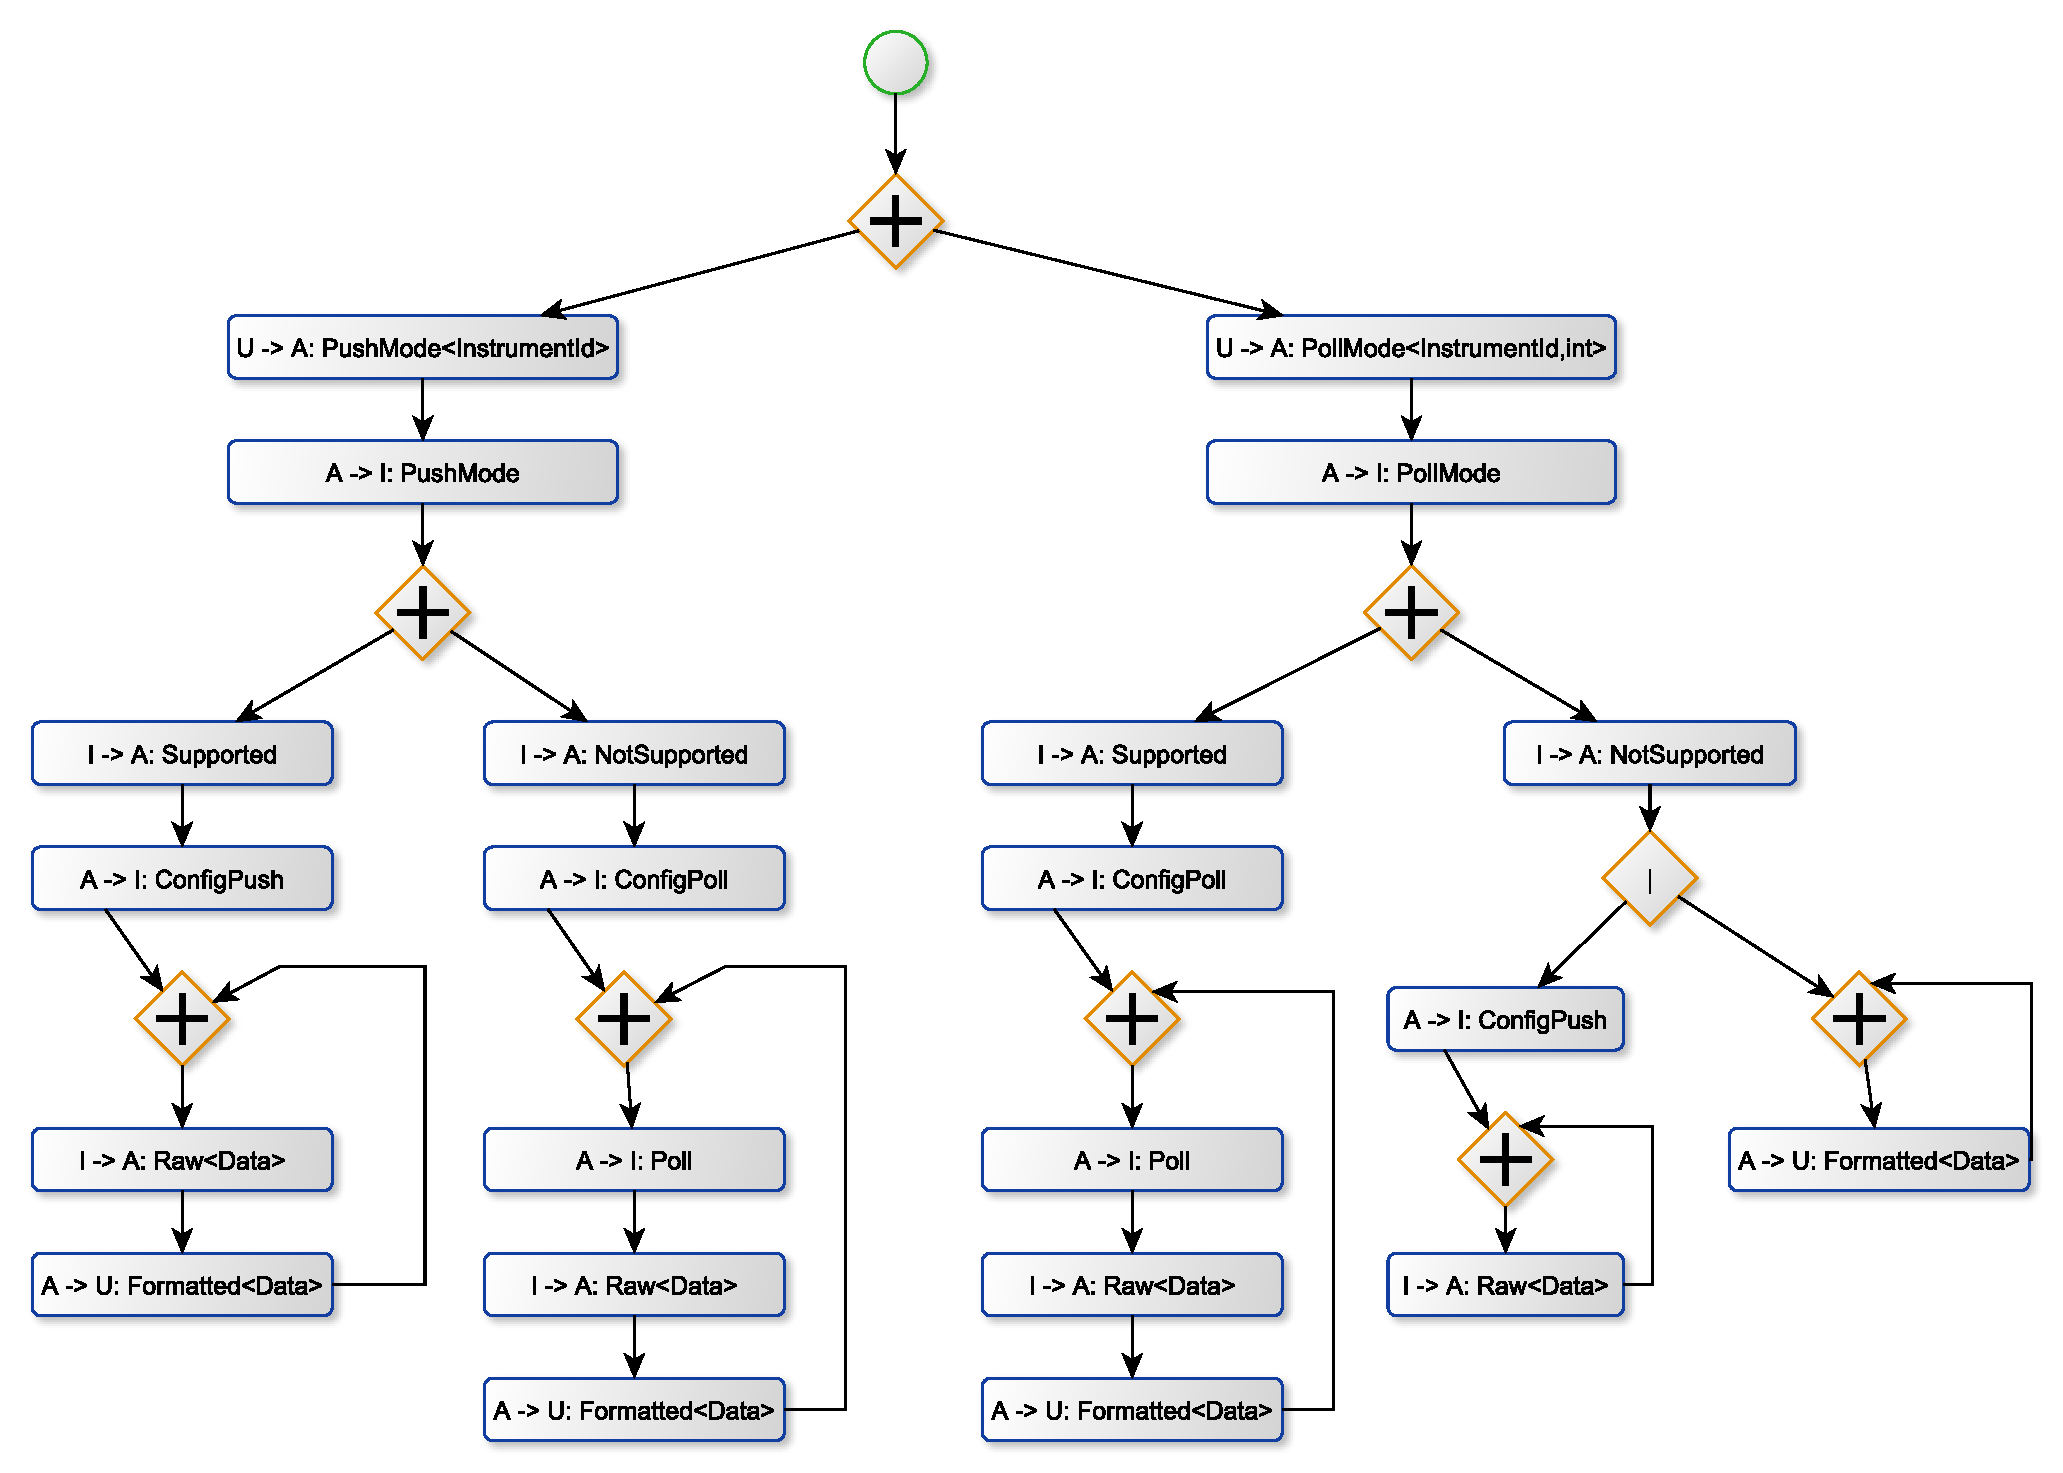
\includegraphics[scale=0.45]{ooi_graph}
\end{center}
\caption{The choreography for the OOI ``Acquire Data from Instrument'' use case}\label{fig:ooi_graph}
\end{figure}

To garantee the safety of this tool, our representation is supported by generalised multiparty session types. Therefore we have established global types for this scenario (Figure \ref{fig:ooi_example1}). 
\begin{figure}[h]
\begin{tabular}{rcrcl}
G =& def & $x_{0}$ &=& $x_{push} + x_{poll}$\\
&& $x_{push}$ &=& U $\rightarrow$ A: PushMode$\langle$ InstrumentId $\rangle ; x_{push1}$\\
&& $x_{push1}$ &=& A $\rightarrow$ I: PushMode ;$ x_{push2}$\\
&& $x_{push2}$ &=& $ x_{pushsup} + x_{pushnsup}$\\
&& $x_{pushsup}$ &=& I $\rightarrow$ A: Supported$ ; x_{pushsup1}$\\
&& $x_{pushsup1}$ &=& A $\rightarrow$ I: ConfigPush$ ; x_{pushsup2}$\\
&& $x_{pushsup2} + x_{pushsup3}$ &=& $x_{pushsup4}$\\
&& $x_{pushsup4}$ &=& I $\rightarrow$ A: Raw$\langle$ Data $\rangle ; x_{pushsup5}$\\
&& $x_{pushsup5}$ &=& A $\rightarrow$ U: Formatted$\langle$ Data $\rangle ; x_{pushsup3}$\\
&& $x_{pushnsup}$ &=& I $\rightarrow$ A: NotSupported$ ; x_{pushnsup1}$\\
&& $x_{pushnsup1}$ &=& A $\rightarrow$ I: ConfigPoll$ ; x_{pushnsup2}$\\
&& $x_{pushnsup2} + x_{pushnsup3}$ &=& $x_{pushnsup4}$\\
&& $x_{pushnsup4}$ &=& A $\rightarrow$ I: Poll$ ; x_{pushnsup5}$\\
&& $x_{pushnsup5}$ &= & I$\rightarrow$ A: Raw$\langle$ Data $\rangle ; x_{pushnsup6}$\\
&& $x_{pushnsup6}$ &=& A $\rightarrow$ U: Formatted$\langle$ Data $\rangle ; x_{pushnsup3}$\\
&& $x_{poll}$ &=& U $\rightarrow$ A: PollMode$\langle$ InstrumentId, int $\rangle ; x_{poll1}$\\
&& $x_{poll1}$ &=& A $\rightarrow$ I: PollMode ;$ x_{poll2}$\\
&& $x_{poll2}$ &=& $ x_{pollsup} + x_{pollnsup}$\\
&& $x_{pollsup}$ &=& I $\rightarrow$ A: Supported$ ; x_{pollsup1}$\\
&& $x_{pollsup1}$ &=& A $\rightarrow$ I: ConfigPoll$ ; x_{pollsup2}$\\
&& $x_{pollsup2} + x_{pollsup3}$ &=& $x_{pollsup4}$\\
&& $x_{pollsup4}$ &=& A $\rightarrow$ I: Poll$ ; x_{pollsup5}$\\
&& $x_{pollsup5}$ &=&  I $\rightarrow$ A: Raw$\langle$ Data $\rangle ; x_{pollsup6}$\\
&& $x_{pollsup6}$ &=& A $\rightarrow$ U: Formatted$\langle$ Data $\rangle ; x_{pollsup3}$\\
&& $x_{pollnsup}$ &=& I $\rightarrow$ A: NotSupported$ ; x_{pollnsup1}$\\
&& $x_{pollnsup1}$& = &$ x_{pollnsup2}\ |\ x_{pollnsup3}$\\
&& $x_{pollnsup2}$ &=& A $\rightarrow$ I: ConfigPush$ ; x_{pollnsup4}$\\
&& $x_{pollnsup4} + x_{pollnsup5}$ &=& $ x_{pollnsup6}$ \\
&& $ x_{pollnsup6}$ &=& I $\rightarrow$ A: Raw$\langle$ Data $\rangle ; x_{pollnsup5}$\\
&& $x_{pollnsup3} + x_{pollnsup7}$ &=&$ x_{pollnsup8}$ \\
&& $ x_{pollnsup8}$ &=& A $\rightarrow$ U: Formatted$\langle$ Data $\rangle ; x_{pollnsup7}$\\
& in $x_{0}$&&&\\
\end{tabular}
\caption{The global protocol for the OOI ``Acquire Data from Instrument'' use case\label{fig:ooi_example1}}
\end{figure}
All $x_{i}$ are state variables. $x_0$ represents the initial state. $ x_{0}$ = $x_{push} + x_{poll}$ is a choice: U will make the choice between continuing with $x_{push}$ or $x_{poll}$. $x_{pushsup2} + x_{pushsup3}$ = $x_{pushsup4}$ is a merge and in this case expresses recursion. $x_{pollnsup1}$ = $ x_{pollnsup2}\ |\ x_{pollnsup3}$ is a fork to model interleaving of actions at $x_{pollnsup2}$ and $x_{pollnsup3}$.

We can see the exact match between the graph representation and the global protocol: indeed, edges are state variables and nodes are the constructions such as interaction, choice, join, etc. For instance, if we focus on the beginning of the protocol declaration:\\

\begin{tabular}{rcrcl}
G =& def & $x_{0}$ &=& $x_{push} + x_{poll}$\\
&& $x_{push}$ &=& U $\rightarrow$ A: PushMode$\langle$ InstrumentId $\rangle ; x_{push1}$\\
&& $x_{poll}$ &=& U $\rightarrow$ A: PollMode$\langle$ InstrumentId, int $\rangle ; x_{poll1}$\\
\end{tabular}

\newcommand{\MYPARAGRAPH}[1]{\paragraph{\textnormal{\textbf{#1}}}}

\definecolor{dkblue}{rgb}{0,0.1,0.5}
\definecolor{dkgreen}{rgb}{0,0.4,0}
\definecolor{dkred}{rgb}{0.4,0,0}


\newcommand{\CODESIZE}{\small}
%\newcommand{\CODESIZE}{\smaller}
\newcommand{\CODESTYLE}{\ttfamily}

\lstset%
{%
	%breakautoindent=true,
	%breaklines=true,
	captionpos=b,
	%columns=fixed,
	columns=flexible, % doesn't give proper space sizes, but fixed is much too fat
	%commentstyle=\itshape\CODESIZE\color{purple},
	commentstyle=\CODESTYLE\footnotesize\color{purple},
	escapeinside={*@}{@*},
	%extendedchars=true,
	float=hbp,
	frame=none,
	% identifierstyle=\color{black},
	language=Java,
	mathescape=true,
	numbers=none, % OLD: Numbers "on" by default: listings inside e.g. tabulars don't seem to work if we give parameters. % Maybe inline \lstset will help?
	numberstyle=\tiny,
	showspaces=false,
	showstringspaces=false,
	showtabs=false,
	stringstyle=\color{teal},
	tabsize=2%, % For some reason, has to be size 9 (equivalently 9 manual spaces) to match \noindent\CODE{12345678}. % maybe due to columns setting
	%xleftmargin=\DEFAULTXLEFTMARGIN % Roughly following the default tabsize.
}

\newcommand{\CODE}[1]{\texttt{\CODESIZE#1}} % Inline code listing (no additional formatting). convention: no colour formatting for inline code.
\newcommand{\GREYCODE}[1]{\CODE{
	%\color{gray}{#1}}} % Problem: braces aren't the same style
	\color{black}{#1}}} % Problem: braces aren't the same style
\newcommand{\SJCODE}[1]
{%
	\lstinline[style=SJ]+#1+%
}

\lstnewenvironment{CODELISTING}% % Listing without numbers or keywords; other parameters as above.
{%
	\onehalfspacing
	%\singlespacing
	\lstset%
	{%
		basicstyle=\CODESTYLE\footnotesize,
		keywordstyle=\CODESTYLE\footnotesize,
		%numbers=none,
		%tabsize=4 % Trying to keep tabsize a variable parameter isn't compatible with indentation conventions. The tabsize is now different to the SJBNF listing, but keep the default xleftmargin to align with BNF listings.
	}
}%
{%
	\doublespacing % Based on the settings of icthesis.sty
}

\lstdefinestyle{SJ}%
{%
	basicstyle   = \CODESTYLE\footnotesize,
	keywordstyle=[1]{
	%\bfseries
	\!\!\!\color{dkblue}
	\CODESTYLE\footnotesize},
	keywordstyle=[2]{
	%\bfseries
	\!\!\!\color{dkgreen}
	\CODESTYLE\footnotesize},
	%numbers     = none,
	%tabsize      = 4, % Same as the tabsize in the CODELISTING environment.
        moredelim=*[s][\footnotesize\color{dkgreen}]{<}{>},
        morekeywords =
	[1]{%
		%terminal, non, extend, RESULT
		protocol, role, choice, at, or, from, to, rec, parallel,
                and, interruptible, by, finish, continue, global, local, self, within
	},
	morekeywords =
	[2]{%
                int,Data,
	%	noalias,
	%	protocol,
	%	cbegin, sbegin, rec, end,
	%	using,
	%	accept, request,
	%	send, receive, receiveInt, receiveDouble, receiveFloat, receiveByte, receiveLong,
	%	outbranch, inbranch, outwhile, inwhile, recursion, recurse,
	%	spawn,
	%	typecase, when,
	%	register, select
	},
       literate={>=}{$\geq\ $}{2}{<=}{$\leq\ $}{2}
}

\lstnewenvironment{SJLISTING}%
{
	\lstset{style=SJ}
}
{
}


%%
% General latex stuff
%
\newcommand{\REF}[1]{\S\,\ref{#1}}

%%
% General code stuff
%
%\newcommand{\CODE}[1]{{\small \texttt{#1}}}
\newcommand{\OPASSIGN}{\, \CODE{:=} \,}
%\newcommand{\OPEQ}{\, \CODE{==} \,}
\newcommand{\OPEQ}{\ensuremath{=}}
\newcommand{\OPDEC}{\CODE{--}}
\newcommand{\OPINC}{\CODE{++}}
\newcommand{\OPSEQ}{\CODE{;}}
\newcommand{\OPNOT}{\ensuremath{\neg}}

%%
% General maths stuff
%\lstnewenvironment{SJLISTING}%
\newcommand{\OLINE}[1]{\ensuremath{\overline{#1}}}  % Overhead line
\newcommand{\SET}[1]{\ensuremath{\{ #1 \}}}         % Set braces
\newcommand{\FUN}[2]{\ensuremath{\mathsf{#1}(#2)}}  % Function call

%%
% General process stuff
%
\newcommand{\KWORD}[1]{\ensuremath{\mathsf{#1}}}
\newcommand{\DTYPE}[1]{\ensuremath{\mathtt{#1}}}  % Data type
\newcommand{\DVAL}[1]{\ensuremath{\mathtt{#1}}}   % Data value
\newcommand{\PPAR}{\ensuremath{\, | \,}}
\newcommand{\PPARGROUP}[1]{\ensuremath{(#1)}}
\newcommand{\PIF}{\ensuremath{\KWORD{if}}}
\newcommand{\PTHEN}{\ensuremath{\KWORD{then}}}
\newcommand{\PELSE}{\ensuremath{\KWORD{else}}}
\newcommand{\PNIL}{\ensuremath{\mathbf{0}}}
\newcommand{\EMPTY}{\ensuremath{\epsilon}}

%%
% General session types stuff
%
\newcommand{\LAB}[1]
	{\ensuremath{#1}}            % "Meta" label: "l"
\newcommand{\LABVAL}[1]
	{\ensuremath{\mathtt{#1}}}   % "Concrete" label: "quit"
\newcommand{\ROLE}[1]
	{\participant{#1}}           % Role/participant
\newcommand{\PARTY}[1]
	{\ensuremath{\mathsf{#1}}}   % Principal
\newcommand{\MSGlxS}[3]
	{\ensuremath{\MSGlx{#1}{#2\!:\!#3}}}  % lab(x:S)
\newcommand{\MSGlx}[2]
	{\ensuremath{#1 (#2)}}              % lab(x)  (variant needed to avoid ":")
\newcommand{\MSGlS}[2]
	{\MSGlx{#1}{#2}}                    % lab(S)
\newcommand{\BRANCH}[1]
	{\ensuremath{\SET{#1}}}         % Branch braces: {...}
\newcommand{\MUREC}[1]
	{\ensuremath{\mu \RECVAR{#1}}}  % Recursion prefix
\newcommand{\RECVAR}[1]
	{\ensuremath{\keyword{#1}}}     % Recursion var.

%%
% General session types stuff
%
\newcommand{\STATEVAR}[1]
	{\ensuremath{\mathtt{#1}}}                % State var.
\newcommand{\ROLEVAR}[2]
	{\ensuremath{\ROLE{#1} . \STATEVAR{#2}}}  % p.x
%\newcommand{\STATEDECL}[2]
	%{\ensuremath{#1 : \DTYPE{#2}}}
\newcommand{\STATEVARDECL}[2]
	%{\ensuremath{\STATEDECL{\STATEVAR{#1}}{#2}}}  % x : Nat
	{\ensuremath{\STATEVAR{#1} : \DTYPE{#2}}}      % x : Nat
\newcommand{\PARTYSTATEDECL}[2]
	{\ensuremath{\ROLE{#1}} : [#2]}                % p[x : Nat, ...]

%%
% Global types
%
\newcommand{\GSEP}{\ensuremath{.}}  % Global type separator
\newcommand{\GLOBAL}[1]
	{\ensuremath{\mathcal{#1}}}       % Global type name: G
\newcommand{\GLOBALi}[2]
	{\ensuremath{\GLOBAL{#1}_{#2}}}   % G_auction
\newcommand{\GSEND}[2]
	{\ensuremath{\ROLE{#1} \rightarrow \ROLE{#2} :}}  % p -> q:
%\newcommand{\GSEND}[5]
	%{\ensuremath{#1 \rightarrow #2 : \MSG{#3}{#4}{#5}}}

% Deprecated: use \BRANCH and \MUREC instead (same for both global and local)
\newcommand{\GBRA}[1]
	{\ensuremath{\SET{#1}}}         % Global branch braces: {...}
\newcommand{\GREC}[1]
	{\ensuremath{\mu \RECVAR{#1}}}  % Global recursion prefix

%%
% Global types for assertions/effects
%
\newcommand{\GLOBALDECL}[1]
	{\ensuremath{((#1))}}             % State var. decl. prefix
\newcommand{\LASS}[1]
	{\ensuremath{\langle #1 \rangle}}  % Left assertion: {...}
\newcommand{\LEFF}[1]
	{\LASS{#1}}                        % Left effect: {...}
\newcommand{\LASSEFF}[2]
	{\ensuremath{\LASS{#1,\, #2}}}     % Left assertion and effect: {..., ...}
\newcommand{\RASS}[1]
	{\ensuremath{\{ #1 \}}}            % Right assertion: <...>
\newcommand{\REFF}[1]
	{\RASS{#1}}                        % Right effect: <...>
\newcommand{\RASSEFF}[2]
	{\ensuremath{\RASS{#1,\, #2}}}     % Right assertion and effect: <..., ...>
\newcommand{\GRECtexA}[4]
	{\ensuremath{\MUREC{#1} \langle #2 \rangle (#3) \{ #4 \}}}
\newcommand{\GRECVARte}[2]
	{\ensuremath{\RECVAR{#1} \langle #2 \rangle}}

%%
% Local types
%
\newcommand{\LSEP}{\ensuremath{.}}  % Local type separator
\newcommand{\LOCAL}[1]
	{\ensuremath{\mathcal{#1}}}       % Local type name: L
\newcommand{\LOCALi}[2]
	{\ensuremath{\LOCAL{#1}_{#2}}}    % L_auction
\newcommand{\LSEND}[1]
	{\ensuremath{\ROLE{#1} \,!\,}}    % p!
\newcommand{\LRECV}[1]
	{\ensuremath{\ROLE{#1} \,?}}      % q!

%%
% Local types for assertions/effeacts
%
\newcommand{\LOCALDECL}[1]
	{\ensuremath{[#1]}}               % State var. decl. prefix
\newcommand{\LRECtexA}[4]
	{\GRECtexA{#1}{#2}{#3}{#4}}
\newcommand{\LRECVARte}[2]
	{\GRECVARte{#1}{#2}}

%%
% Session processes (1)
%
\newcommand{\POSEP}{\ensuremath{;}}  % After output prefixes
\newcommand{\PESEP}{\ensuremath{;}}  % Separator for effects
\newcommand{\PSEP}{\ensuremath{.}}   % Others: input prefixes, recursion, etc.
\newcommand{\PINIT}[1]
	{\ensuremath{\mathsf{#1}}}         % Initial process
\newcommand{\PINITi}[2]
	{\ensuremath{\mathsf{#1}_{#2}}}    % e.g. initial P_Server
%\newcommand{\PRUNT}
	%{\ensuremath{#1}}
\newcommand{\PREQ}[4]
	{\ensuremath{\OLINE{#1} \langle #2 [\ROLE{#3}] : \GLOBAL{#4} \rangle}}
                                                                % a~<x[p]:G>
\newcommand{\PACC}[4]
	{\ensuremath{#1 ( #2 [ \ROLE{#3} ] : \GLOBAL{#4} )}}          % a(x[p]:G)
\newcommand{\PSEND}[5]
	{\ensuremath{#1 [\ROLE{#2}, \ROLE{#3}] \,!\, \LAB{#4} \langle #5 \rangle}}
	                                                              % k[p,q]!l<e>
\newcommand{\PRECV}[3]
	{\ensuremath{#1 [\ROLE{#2}, \ROLE{#3}] \,?\,}}                % k[p,q]?
\newcommand{\PRECX}[1]
	{\ensuremath{\mu #1}}                            % mu X
\newcommand{\PRECXx}[2]
	{\ensuremath{\PRECX{#1} (#2)}}                   % mu X (x) ...
\newcommand{\PRECe}[1]
	{\ensuremath{\langle #1 \rangle}}                % ... <e>
\newcommand{\PRECVARX}[1]
	{\ensuremath{#1}}                                % X
\newcommand{\PRECVARXe}[2]
	{\ensuremath{\PRECVARX{#1} \langle #2 \rangle}}  % X<e>

% Deprecated: syntax change
\newcommand{\PRECx}[2]
	{\ensuremath{\MUREC{#1} (#2)}}
\newcommand{\PRECtx}[2]
	{\ensuremath{\MUREC{#1} (#2)}}      % mu t (x) ...
\newcommand{\PRECVARte}[2]
	{\GRECVARte{#1}{#2}}

%%
% Session processes (2)
%
\newcommand{\PNEWKW}{\KWORD{new}}
\newcommand{\PREGKW}{\KWORD{reg}}
\newcommand{\PINKW}{\KWORD{in}}
%\newcommand{\PWITHKW}{\KWORD{with}}
%\newcommand{\PINVITE}[2]
	%{\ensuremath{\mathtt{I}(\mathcal{#1}[\ROLE{#2}])}}          % I(G[p])
\newcommand{\PNEWs}[4]
	{\ensuremath{\PNEWKW\, (\AT{#1}{#2}, \ROLE{#3}) \,\PINKW\, #4}}  % new (s:G, p) in P
\newcommand{\PNEWa}[4]
	{\ensuremath{\PREGKW\, \AT{#1}{#2}[\ROLE{#3}] \,\PINKW\, #4}}
                                                        % new a:I(G[p]) in P
\newcommand{\PNEWp}[4]
	{\ensuremath{\PNEWKW\, \AT{#1}{#2} \,\KWORD{with}\, [#3] \,\PINKW\, #4}}
                                           % new \alpha:\Gamma with [P] in Q

% Deprecated: not needed
%\newcommand{\PJOINKW}{\KWORD{join}}
\newcommand{\PJOIN}[2]
	{\ensuremath{\KWORD{join}\, #1[#2]}}  % join s[p]

%%
% Session processes (3)
%
\newcommand{\PLOCK}
	{\ensuremath{\blacktriangledown \,}}
\newcommand{\PUNLOCK}
	{\ensuremath{\blacktriangle}}
\newcommand{\PGET}[2]
	{\ensuremath{#1 \OPASSIGN get(\STATEVAR{#2})}}  % x := get(f)
\newcommand{\PPUT}[2]
	{\ensuremath{put(#1, \STATEVAR{#2})}}           % put(f, e)
\newcommand{\PLRECV}[3]
	{#1 [\ROLE{#2}, \ROLE{#3}] \, ? \blacktriangledown}

%%
% Session processes (4)
%
\newcommand{\PSNET}[1]
	{\ensuremath{#1}}     % Static network: N
\newcommand{\PSNETi}[2]
	{\ensuremath{#1_{#2}}}
%\newcommand{\PDNET}[1]
	%{\ensuremath{\mathcal{#1}}}
\newcommand{\PICHAN}[2]
	{\ensuremath{\mathtt{I}(#1 [\ROLE{#2}])}}
\newcommand{\POCHAN}[2]
	{\ensuremath{\mathtt{O}(#1 [\ROLE{#2}])}}
\newcommand{\PNETQUEUE}[2]
	{\ensuremath{\langle #1 ; #2 \rangle}}

\newcommand{\RAYCOMMENT}[1]{~\\ \textbf{RAY:} #1}



\begin{figure}[p]
\centering
\begin{tabular}{ll}
{\lstset{numbers=left}
\begin{SJLISTING}
// U is User, A is ION Agent, I is Instrument
global protocol DataAcquisition(role U, role A, role I) {
	interruptible {		choice at U { *@\label{line:userchoiceopen}@*
						PushMode(InstrumentId) from U to A;
						PushMode from A to I;
						choice at I {
							Supported from I to A;
							ConfigPush from A to I;
							rec PUSH { *@\label{line:firstrecursion}@*
								Raw(Data) from I to A;
								Formatted(Data) from A to U;
								continue PUSH;
							}
						} or {
							NotSupported from I to A;
							ConfigPoll from A to I;
							rec POLL {
								Poll from A to I;
								Raw(Data) from I to A;
								Formatted(Data) from A to U;
								continue POLL;
						}	}
					} or { *@\label{line:userchoiceor}@*
						PollMode(InstrumentId,int) from U to A;
						PollMode from A to I;
						choice at I {
							Supported from I to A;
							ConfigPoll from A to I;
							rec POLL {
								Poll from A to I;
								Raw(Data) from I to A;
								Formatted(Data) from A to U;
								continue POLL;
							}
						} or { *@\label{line:pollnotsupportedopen}@*
							NotSupported from I to A;
							parallel {
								ConfigPush from A to I;
								rec PUSH {
									Raw(Data) from I to A;
									continue PUSH;
								}
							} and {
								rec POLL {
									Formatted(Data) from A to U;
									continue POLL;	}
						}	} *@\label{line:pollnotsupportedclose}@*
					} *@\label{line:userchoiceclose}@*
	} by U with Stop
}
\end{SJLISTING}}
&
\end{tabular}
\caption{The Scribble global protocol for the OOI ``Acquire Data from Instrument'' use case\label{fig:ooi_example2}}
\end{figure}

\begin{figure}[h]
\begin{center}
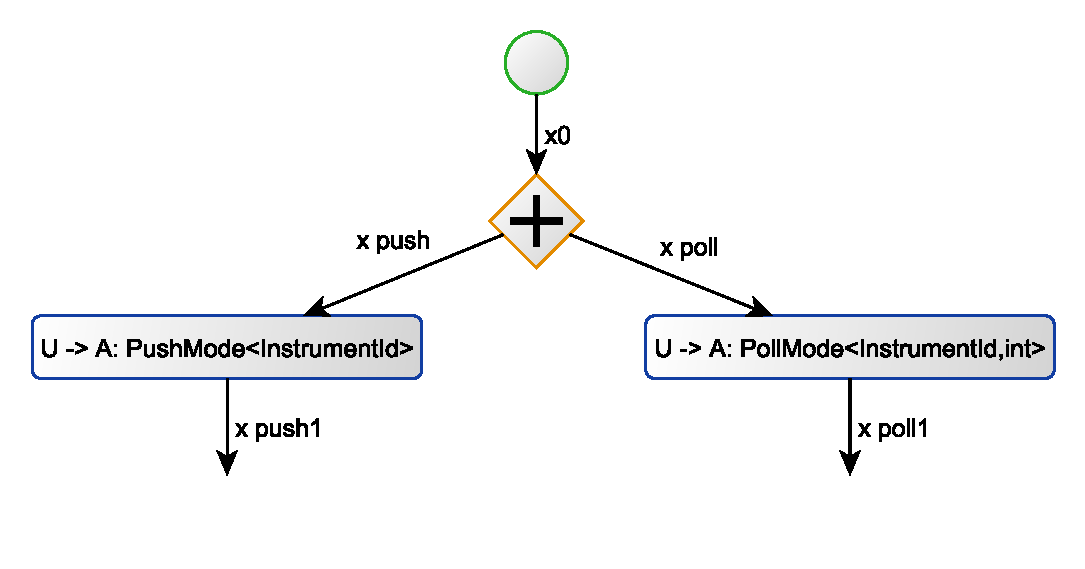
\includegraphics[scale=0.8]{ooi_graph_details}
\end{center}
\caption{Mapping between global protocol and graph}
\label{fig:ooi_example1_details}
\end{figure}

~~\\
the mapping between global protocol and graph could be represented as in Figure \ref{fig:ooi_example1_details}.

Furthermore, there exists a programming language, called Scribble, that aims at providing a simple language, as its name states it, to express global protocols as well as local protocols. Besides, a complete tool chain from global protocols in Scribble to the generation of the classes for the end-point programs is being developed. It uses the projection from global to local protocols. Our goal is to add the first step of this tool chain with a graph representation. For this purpose we want to establish a clear correspondence between global protocols in Scribble and our graphical notations. As an example, we give in Figure \ref{fig:ooi_example2} the corresponding global protocol in Scribble of our scenario. The part of the protocol we presented in more details in Figure \ref{fig:ooi_example1_details} corresponds to this extract from the program in Scribble:\\

\begin{tabular}{ll}
\begin{SJLISTING}
choice at U { *@\label{line:userchoiceopen}@*
	PushMode(InstrumentId) from U to A;
} or { *@\label{line:userchoiceor}@*
	PollMode(InstrumentId,int) from U to A;
}
\end{SJLISTING}
& Code in Scribble corresponding to Figure \ref{fig:ooi_example1_details}
\end{tabular}




\section*{Contributions}
\addcontentsline{toc}{section}{Contributions}

We begin with exposing in this report all the background work we have done to obtain, as well as an overview of the on-going research, a deep knowledge in session types. This was a prerequisite to become familiar with the key elements: session types, Scribble language. 

The main topic is the session types. Even if some features of sessions are related to Pi-calculus, the theory behind is based on different elements. To understand step by step where generalised multiparty session types (section 1.1.3) come from, we first study binary session types (section 1.1.1) and work on simple examples. Then we turn to multiparty session types (section 1.1.2) for which the major part of understanding work has to be done. Common features to all these topics are verification issues. We will look at some specific work in section 1.1.4. The second key element of our project is the Scribble language (section 1.2.1). In order to build our graph notations in correspondence with it, we studied the syntax (section 1.2.2) and its features (section 1.2.3). To conclude the background work, we looked at work related to implementation issues based on session types (section 1.3). The implementation is indeed a great part of the work once theory has been developed.

We proceed with our work and in particular the design we have chosen for graphs (chapter 2): we start from general principles we obtained from the background work (section 2.1) to continue with a discussion about existing representations (section 2.2) before presenting our notations (section 2.3).

Once our notations have been set, the major work concerns the development (chapter 3). We expose our general architecture as an overview (section 3.1) and then get into more details to explain how from a global protocol in Scribble we obtain a graph (section 3.2) and vice versa (section 3.3).

Then we present our implementation (chapter 4): we explain first the general structure of the code (section 4.1), then the library in Python we have developed to create the needed graphical objects (section 4.2) and finally some details about both ways of the correspondence (sections 4.3 and 4.4).

To summarize our contributions concerning the graph representation:
\begin{itemize}
\item We establish notations for graphs that correspond to Scribble global protocol and which are supported by generalised multiparty session types.
\item We provide the implementation of a software tool to perform the transformation from Scribble global protocol into graph, and vice versa. The correspondence is based on a library of graphical objects in Python.
\end{itemize}
~~\\
In a second time, to go further, we extended our work to provide a notion of time to such protocols and graphs. In chapter 5, we introduce this new feature with general principles (section 5.1), the corresponding design (section 5.2) with the extension of the Scribble language (section 5.3), as well as the changes on the implementation (section 5.4). To concretise our work, we developed timed global protocol (chapter 6). Starting from related work (section 6.1), we established our own syntax (section 6.2). We present the expressiveness of our syntax (section 6.3), before presenting some key results we obtained or we conjecture (section 6.4).

To summarize our contributions regarding time:
\begin{itemize}
\item We extend the syntax for Scribble protocols, as well as for generalised local and global types.
\item We clearly define structures to express timeouts for message passing, delays and other time constraints.
\item We define a temporal satisfiability criterion for clock conditions and conjecture progress and error-freedom properties for processes.
\end{itemize}

Finally, we have evaluated the expressiveness and usability of our graph representation (chapter 7). We define a method for the evaluation (section 7.1), and we perform the implementation of several test cases (section 7.2). As a result, we achieve to demonstrate the conformance of our graphical representation to well-formed global protocols (section 7.3). We conclude with a summary of what we have achieved, some feedbacks on the project with the improvements that can be made and possible future work.


\chapter{Background}



\section{Session types}

As we have seen in the introduction there is a need in distributed programming for a clear structure to express conversation.

A session is a structure to encapsulate a safe communication scheme between two or more peers in a context of distributed processes. A typing system is associated to this structure in order to statically check the programs from the processes, in particular safety and consistency.
A session is introduced to describe a sequence of interactions between the processes.

As the case of two processes was first studied, we begin with exposing the binary session types to get the idea of session types. Then it has been extended to more than two processes with multiparty session types in order to express more complex interactions. Therefore we will continue with a detailed presentation of multiparty session.


\subsection{Binary session types}
\begin{table}[tb]
\centering
\begin{tabular}{rclr}
 \PP & ::=  &  request a(k) in \PP   &   {Session Request}\\
     & \sep & accept a(k) in \PP   &   {Session Acceptance}\\
     & \sep & \outS{\Ik}\e\PP &    {Data sending}\\
     & \sep & \inpS{\Ik}\x\PP &    {Data reception}\\
     & \sep & throw \Ik[\Ik']; \PP & {Channel Sending}\\
     & \sep & catch \Ik(\Ik') in \PP &  {Channel Reception}\\
     & \sep & \Ik $\vartriangleleft$ ;{\PP} & {Label Selection}\\
     & \sep & \Ik $\vartriangleright \{  l_{1}:{\PP}_{1} \| ... \|  l_{n}:{\PP}_{n} \} $ & {Label Branching}\\[1mm]
     & \sep & \ifthenelse{\e}{\PP}{\Q} & {Conditional Branch}\\
      & \sep & \PP \pc \Q  & {Parallel}\\
      & \sep & inact & {Inaction}\\
      & \sep & \nuc{\Iu}{\PP} & {Name/Channel Hiding}\\
      & \sep & \defD \PP & {Recursion}\\
      & \sep & \X[\e\Ik] & {Process Variables}
\\
\\[2mm]
\e   & ::= & \Ic & {Constant}  \\
&  \sep & \e+\e' \sep  \e-\e' \sep \e+\e' \sep\NOT{\e} $\ldots$x
&{Expression}\\
\DD   & ::= & \Ddef &{Declaration}\\
\end{tabular}
\ \vspace{1mm}
\caption{Syntax for user-defined processes}\label{tab:syntaxB}
\end{table}

Binary session types contain the expected communication features, as studied in the Models of Concurrent Computation course: value sending and receiving, recursion, choice of interactions. What is new is the session initiation and session delegation.

We proceed with an example that we have established to explain in more details the syntax (Table \ref{tab:syntaxB}), operational semantics and typing system involved in binary sessions.
We consider the case of a client using the National Rail website to book a train ticket. The scenario is as follows:
\begin{itemize}
\item The client first chooses the destination.
\item Then the service (National Rail) contacts the right company to delegate the deal. The client will continue the transaction, unaware that she now communicates directly with the company.
\item The client and the company exchange the date, the price and the money.
\end{itemize}
Here is the syntax for the system made up of one client, {\em Client}, the National Rail Service, {\em NRS}, and one of the companies, {\em Company}.
\begin{center}
\begin{tabular}{lrcl}
def&Client &=& request a(k) in  k $\vartriangleleft$ bristol;k!(date);k?(price);k!(money);inact\\
and&NRS &=& accept a(v) in k $\vartriangleright$ \{bristol:request c(k') in throw k'[v];NRS $\| ...\|$ newcastle: ... \}\\
and&Company &=& accept c(k') in catch k'[k] in k?(date);k!(price);k?(money);Company\\
in& & &Client | NRS | Company\\
\end{tabular}
\end{center}
The three first lines introduce the recursion that is used for the process defined in the last line. The first line specifies that a client first requests a session with the national rail service (\emph{request a(k) in}), then selects the destination labelled Bristol (\emph{k $\vartriangleleft$ bristol;}), and finally sends the date (\emph{k!(date);}), receives the corresponding price (\emph{k?(price);}) and sends the money (\emph{k!(money);}) before halting (\emph{inact}). The second line describes  the interactions from the side of the national rail service: it accepts the request of session (\emph{accept a(v) in k }) and then has a branching choice (\emph{k $\vartriangleright$ \{ ... \}}). We only specify the case for the label called Bristol: NRS requests a new session with the corresponding company (\emph{request c(k') in}) and delegates the deal (\emph{throw k'[v];}), before being available again for other interactions. The third line specifies that a company first accepts the request for a new session (\emph{accept c(k') in}) then receives the delegation of the deal (\emph{catch k'[k] in }) and finally operates the receiving of the date (\emph{k?(date);}), the sending of the price (\emph{k!(price);}) and the receiving of the money (\emph{k?(money);}), before being available again.

Rather than exposing all the tables for operational semantics and typing system, that can be found in \cite{honda1998language,yoshida2007language}, we apply the rules to reduce our example. Let call \PP ~the system above defined and D the declaration for recursion inside \PP, and apply to it the reduction rules.\\
~~\\
\begin{tabular}{lclr}
\PP& $\rightarrow$ &def D in ($\nu$ k) ( k $\vartriangleleft$ bristol;k!(date);k?(price);k!(money);inact | & [Link]\\
&& k $\vartriangleright$ \{bristol:request c(k') in throw k'[k];NRS $\| ...\|$ newcastle: ... \}) |&  \\
&&accept c(k') in catch k'[k] in k?(date);k!(price);k?(money);Company&  \\
& $\rightarrow$  & def D in ($\nu$ k) (k!(date);k?(price);k!(money);inact | request c(k') in throw k'[k];NRS) |&[Label]\\
&&accept c(k') in catch k'[k] in k?(date);k!(price);k?(money);Company&\\
& $\rightarrow$  & def D in ($\nu$ k) (k!(date);k?(price);k!(money);inact | ($\nu$ k')(throw k'[k];NRS |& [Link]\\
&&catch k'[k] in k?(date);k!(price);k?(money);Company))&\\
& $\rightarrow$  & def D in ($\nu$ k) (k!(date);k?(price);k!(money);inact | & [Pass]\\
&& ($\nu$ k')(NRS |  k?(date);k!(price);k?(money);Company))&\\
& $\rightarrow$  & def D in ($\nu$ k) (k?(price);k!(money);inact |  ($\nu$ k')(NRS | k!(price);k?(money);Company))& [Com]\\
& $\rightarrow$  & def D in ($\nu$ k)( k!(money);inact | ($\nu$ k')(NRS |  k?(money);Company))&[Com]\\
& $\rightarrow$  & def D in ($\nu$ k) (inact |  ($\nu$ k')(NRS | Company))& [Com]\\
& $\equiv$  & def D in (NRS | Company) & \\
\end{tabular}
~ ~\\
Besides the above specified reduction rules, we used [Def] at each step and [Str] at the second [Link] step in order to put the third part inside ($\nu$ k).

The process \PP~is also typable with respect to the typing system. We give here two results of this typing:
\[ \der \Ga { k \vartriangleleft bristol;k!(date);k?(price);k!(money);inact}\D,k:\oplus \{ bristol:![nat];?[nat];![nat];end\}\]
\[ \der \Ga {catch~ k'[k] in~ k?(date);k!(price);k?(money);inact}\D,k':?[~ ![nat];?[nat];![nat];end~ ];end\]

Therefore binary session types allow expressing complex communication structure between two peers and to ensure its safety. Nevertheless, in a real world context, conversations usually involve more than two entities. To solve this issue, one can first think of modelling interactions between more than two processes using binary session types for each pair of them in the same way as the previous example. It appears however that it removes the desired clarity of the structure. Furthermore it cannot express the situation as a whole but only separate interactions. That is why researchers introduce multiparty session types.



\subsection{Multiparty session types}


\subsubsection{Overview}
A multiparty session describes the interactions between several processes. Besides specifying the user-defined processes involved in a session, we have to define, at a higher level, a global protocol that ensures the coherence of the session. The typing system allows specifying these two levels: first there is a global type and then projections of this global type to each endpoint processes, the local types. 

In multiparty session programming, a developer will have to define the global type and the user-defined processes. The key step in the methodology consists then of checking the correspondence between the projections from the global type and the type of the endpoint programs. We summarize the structure of multiparty session types in Figure \ref{fig:mpst}.

\begin{figure}[h]
\begin{center}
\includegraphics{mpst}
\caption{General structure for multiparty session types}\label{fig:mpst}
\end{center}
\end{figure}

With respect to the procedure, we get several properties: type safety, session fidelity, progress, linearity. Also the structure of sessions makes it possible to deal with interferences and interleaving of interactions among participants.

To describe with more details and more formally what is explained above, we look at the example of the three buyers protocol and then introduce syntax, operational semantics and the typing system, as defined in \cite{coppoglobal}.


\subsubsection{The three buyers protocol example}
We first introduce the calculus through the example of the three-buyer protocol, which includes the expected communication features, as well as session-multicasting and dynamically merging two conversations. This example is extracted from \cite{coppoglobal}. "The overall scenario  proceeds as follows.
\begin{enumerate}
\item Alice sends a book title to Seller, then Seller sends back a quote to Alice and Bob. Then Alice tells Bob how much she can contribute.
\item If the price is within Bob's budget, Bob notifies both Seller and Alice he accepts, then sends his address, and Seller sends back the delivery date.
\item If the price exceeds the budget, Bob asks Carol to collaborate together by establishing a new session. Then Bob sends how much Carol must pay, then {\em delegates} the remaining interactions with Alice and Seller to Carol.
\item  If the rest of the price is within Carol's budget, Carol accepts the quote and notifies Alice, Bob and Seller, and continues the rest of the protocol with Seller and Alice transparently, {\em as if she were Bob}. Otherwise she notifies Alice, Bob and Seller to quit the protocol.\vspace{-2mm}
\end{enumerate}
Figure~\ref{fig:threebuyers} depicts an execution of the above protocol where Bob asks Carol to collaborate (by delegating the
remaining interactions with Alice and Seller) and the transaction terminates successfully.

\begin{figure}[tb]
\begin{center}
\includegraphics[scale=0.25]{three_buyer_protocol}
\end{center}
\caption{The three buyer protocol interactions}\label{fig:threebuyers}
\end{figure}

Then multiparty session programming consists of two steps: (1) specifying the intended communication protocols using global types,
and (2) implementing these protocols using processes. The specifications of the three-buyer protocol are given as two separated global types: one is $G_a$  among Alice, Bob and Seller and the other is $G_b$ between Bob and Carol. We write principals with legible symbols though they will actually be coded by numbers: in $G_a$ we have  $\participant{A}=1$, $\participant{B}=2$, and $\participant{S}=3$, while in $G_b$ we have $\participant{B}=2$, $\participant{C}=1$.\\[0.5mm]
\newcommand{\nm}[1]{{\texttt{\scriptsize #1.}}}

{\small
$
\begin{array}{ll}
G_a =&  G_b =\\
\begin{array}{llllll}
 \nm{1}& \participant{A} & \redsym & \participant{S}: & \langle \kf{string}\rangle.\\
  \nm{2}&\participant{S}  & \redsym & \{\participant{A},\participant{B}\}: & \langle \mathsf{int}\rangle .\\
  \nm{3}&\participant{A} & \redsym & \participant{B}:& \langle \mathsf{int}\rangle .\\
  \nm{4}&\participant{B} & \redsym & \{\participant{S},\participant{A}\}: & \{\mathsf{ok:}
 \participant{B} \redsym \participant{S}:\langle \kf{string}\rangle.\\
 \nm{5}& & & & \quad\quad \ \participant{S} \redsym
\participant{B}:
\langle \kf{date}\rangle ;\End\\
\nm{6} & & & & \ \mathsf{quit}: \End\}\\
\\
\end{array}
&
\begin{array}{llllll}
 \nm{1} & \participant{B}& \redsym & \participant{C}:&\langle \kf{int}\rangle .\\
 \nm{2}      &\participant{B}& \redsym & \participant{C}:&\langle T \rangle .\\
 \nm{3}     &\participant{C}& \redsym & \participant{B}: &
\{\mathsf{ok}:
\End, \quad \mathsf{quit}: \End\}.\\[1mm]
 & & & & \hspace{-1.8cm}
T=\\
 & & & & \hspace{-1.8cm}\
\oplus \langle\{\participant{S},\participant{A}\},\\
 & & & & \hspace{-1.8cm} \  \ \ \ \ \{\mathsf{ok}:!\langle
\participant{S},\kf{string}\rangle; ?\langle
\participant{S},
\kf{date}\rangle;
\End,\\
 & & & & \hspace{-1.8cm} \ \ \ \ \ \ \mathsf{quit}: \End\}\rangle\\[0.5mm]
\end{array}
\end{array}
$\\[0.5mm]
}

The types give a global view of the two conversations, directly abstracting the scenario given by the diagram. In $G_a$, line 1 denotes $\participant{A}$ sends a string value to $\participant{S}$. Line 2 says $\participant{S}$ multicasts the same integer value to $\participant{A}$ and $\participant{B}$ and line 3 says that $\participant{A}$ sends an integer to $\participant{B}$. In lines 4-6 $\participant{B}$ sends either $\mathsf{ok}$ or $\mathsf{quit}$ to $\participant{S}$ and $\participant{A}$. In the first case $\participant{B}$ sends a string to $\participant{S}$ and receives a date from $\participant{S}$, in the second case there are no further communications.

Line 2 in $G_b$ represents the delegation of the capability specified by the session type $T$ of channels (formally defined later) from $\participant{B}$ to $\participant{C}$ (note that \participant{S} and \participant{A} in $\T$ concern the session on \Ia).

Figure~\ref{tbe} gives the code, associated to $G_a$ and $G_b$, for \participant{S,\,A,\,B} and \participant{C} in a ``user'' syntax
formally defined later\footnote{In the examples we will use the following font conventions: variables (bound by an input action) are in \textit{italics} and constants are in \constf{sans serif}; string literals are in \texttt{monospace} font and double quoted. }: 
\begin{figure}
\begin{tabular}{rcl}
\participant{S} & $=$ & $\bar{a}[3](y_3).y_3?(\textit{title}); y_3!\langle \constf{quote} \rangle; y_3\& \{\mathsf{ok}:y_3?(\textit{address}); y_3!\langle \constf{date} \rangle; \inact, \ \mathsf{quit}: \inact\}$ \\[2mm]
\participant{A} & $=$ & $a[1](y_1).y_1!\langle \texttt{"Title"} \rangle; y_1?(\textit{quote});y_1!\langle \textit{quote} \ \mathsf{div} \ 2\rangle; y_1\& \{\mathsf{ok}:\inact, \ \mathsf{quit}: \inact\}$ \\[2mm]
\participant{B} &  $=$ & $a[2](y_2).y_2?(\textit{quote}); y_2?(\textit{contrib});$\\
   &     & \indent $\mathsf{if}~(\textit{quote - contrib} < 100)  ~\mathsf{then}~\ y_2 \oplus \mathsf{ok}; y_2!\langle  \texttt{"Address"}\rangle;y_2?(\textit{date});  \inact$\\
& &  \indent $\mathsf{else}~\sr\Ib 2{\z_2 }{\z_2 !\langle \textit{quote - contrib - }99\rangle; \z_2 !\langle\! \langle y_2 \rangle\!\rangle ; z_2 \& \{\mathsf{ok}: \inact, \ \mathsf{quit}: \inact\}}$\\[2mm]
\participant{C} &  $=$ &  $\sa \Ib 1 {z_1 }{\z_1 ?(x); \z_1 ?(\! (t)\!)};$\\
   &      & $%\nind
 \mathsf{if}~(x < 100)~\mathsf{then}~z_1 \oplus \mathsf{ok}; t \oplus \mathsf{ok}; t!\langle \texttt{"Address"}\rangle;t?(\textit{date}); \inact$\\ 
& & % \nind
$\mathsf{else}~z_1 \oplus \mathsf{quit};t \oplus \mathsf{quit}; \inact$
\end{tabular}\\[0.5mm]
\caption{The three buyer example}\label{tbe}
\end{figure}
Session name $\Ia$ establishes the session corresponding to $\G_\Ia$. \participant{S} initiates a session involving three bodies as third participant by $\bar{a}[3](y_3)$: \participant{A} and \participant{B} participate as first and second participants by $a[1](y_1)$ and $a[2](y_2)$, respectively. Then \participant{S}, \participant{A} and \participant{B} communicate using the channels $y_3$, $y_1$ and $y_2$, respectively. Each channel $\y_\p$ can be seen as a port connecting participant $\p$ with all other ones; the
receivers of the data sent on $\y_\p$ are specified by the global type (this information will be included in the runtime code). The
first line of $\G_\Ia$ is implemented by the input and output actions $y_3?(\textit{title})$ and $y_1!\langle \texttt{"Title"}
\rangle$. The last line of $\G_\Ib$ is implemented by the branching and selection actions $z_2\& \{\mathsf{ok}: \inact, \ \mathsf{quit}: \inact\}$ and $z_1\oplus \mathsf{ok}$, $z_1\oplus \mathsf{quit}$.

In \participant{B}, if the quote minus \participant{A}'s contribution exceeds 100\euro\ (i.e., $\textit{quote - contrib} \geq 100$), another session  between \participant{B} and \participant{C} is established dynamically through shared name $\Ib$. The delegation is performed by passing the channel $y_2$ from \participant{B} to \participant{C} (actions $\z_2!\langle\! \langle y_2 \rangle\!\rangle$ and $\z_1?(\! (t)\!)$), and so the rest of the session is carried out by \participant{C} with \participant{S} and \participant{A}." 

We chose to study this example as it is widely-used in the literature. This example illustrates indeed how multiparty session types are used for such a protocol and guarantees safe communication. To become more familiar with multiparty session types, we worked on this example and applied to it the semantics rules, as we did for binary session types.


\subsubsection{Syntax and semantics}
The real improvement in multiparty session types, compared to binary session types, is the notion of global protocol, which will be used as a choreography for the whole system. The syntax for global protocols can be found in \cite{coppoglobal}.
The grammar for processes, ranged over by $\PP, \Q\dots$, and for expressions, ranged over by $\e,\e',\dots$, similar to the binary session case, is given by the Table~\ref{tab:syntaxM}.

The rules for operational semantics are also from \cite{coppoglobal} and given in Tables~\ref{tab:structcong} (\cas\ ranges over \Ia, \s\ and $z$ ranges over
\at{\va}, \si\s\p\ and $l$.),~\ref{tab:reduction}.
% expose examples of reduction that we did.

\begin{table}[tb]
\centering
\begin{tabular}{lll}
\begin{tabular}{rclr}
 \PP & ::=  & \sr\uu \pn\y\PP   &   {Multicast Request}\\
     & \sep & \sa\uu\p\y\PP   &   {Accept}\\
     & \sep & \outS{\y}\e\PP &    {Value sending}\\
     & \sep & \inpS{\y}\x\PP &    {Value reception}\\
     & \sep & \sdS{\y}{\z} \PP & {Session delegation}\\
     & \sep & \rdS{\y}{\z}\PP &  {Session reception}\\
     & \sep & \lselS{\y}{l}{\PP} & {Selection}\\
     & \sep & \lbranchS{\y} & {Branching}\\[1mm]
\uu & ::= & $\x$ \ \sep \Ia & {Identifier}\\
\va & ::= & \Ia \ \sep \true  \ \sep \false & {Value}\\
\end{tabular}
&
&
\begin{tabular}{rclr}
      & \sep & \ifthenelse{\e}{\PP}{\Q} & {Conditional}\\
      & \sep & \PP \pc \Q  & {Parallel}\\
      & \sep & \inact & {Inaction}\\
      & \sep & \nuc{\Ia}{\PP} & {Hiding}\\
      & \sep & \defD \PP & {Recursion}\\
      & \sep & \proccall{\X}{\e}{\y} & {Process call}
\\
\\[2mm]
\e   & ::= & \va \ \sep \x  \\
&  \sep & \AND{\e}{\e'} \sep \NOT{\e} $\ldots$
&{Expression}\\
\DD   & ::= & \Ddef &{Declaration}\\
\end{tabular}
\end{tabular}
\ \vspace{1mm}
\caption{Syntax for user-defined processes}\label{tab:syntaxM}
\end{table}

\begin{table}[tb]
\centering
\begin{tabular}{c}
  $P \Par \textbf{0}\equiv P\ \ \ \ \ P \Par Q\equiv Q \Par P\ \ \ \ \
  (P \Par Q) \Par R\equiv P \Par (Q \Par R)$\\
  \\
  $(\nu \cas)P \Par Q\equiv (\nu \cas)(P \Par Q)\ \ \ \ \ \ \text{if}\ \cas\notin
  \freen{\Q}$\\
  \\
  $(\nu \cas\cas')P\equiv (\nu \cas'\cas)P\ \ \ \ \ \ (\nu \cas)\textbf{0}\equiv \textbf{0}\ \
  \ \ \ \ \defD\textbf{0}\equiv \textbf{0}$\\
  \\
  $\defD(\nu \cas)P\equiv (\nu \cas)\defD\PP\ \ \ \ \ \ \text{if}\ \cas\notin
  \freen{D}$\\
  \\
  $(\defD\PP) \Par Q\equiv \defD{(P \Par Q)}\ \ \ \ \ \ \text{if}\ \dpv{D}\cap
  \fpv{Q}=\emptyset$\\
  \\
  $\defD(\defDp\PP)\equiv \defIn{\AND{D}{D'}}\PP\ \ \ \ \ \ \text{if}\
  \dpv{D}\cap \dpv{D'}=\emptyset$\\
  \\
   $\mqueue{\s}{
   \qhead
    {
        \qcomp
        {\trival{z}{\pset}{\q}}
        {\trival{z'}{\pset'}{\q'}}
    }
   } \equiv
   \mqueue{\s}{
   \qhead
    {
        \qcomp
        {\trival{z'}{\pset'}{\q'}}
        {\trival{z}{\pset}{\q}}
    }
   }$ 
   $\qquad \text{if $\pset \cap \pset'=\emptyset$ or $\q \ne \q'$}$\\
   \\
   $\mqueue{\s}{
   \qhead
    {
        {\trival{z}{ \pset}{\q}}
    }
   } \equiv
   \mqueue{\s}{
   \qhead
    {
        \qcomp
        {\trival{z}{\pset'}{\q}}
        {\trival{z}{\pset''}{\q}}
    }
   }$ 
   $\qquad \text{where $\pset = \pset' \cup \pset''$ and }\pset' \cap \pset''=\emptyset$
\end{tabular}
\caption{Structural equivalence}\label{tab:structcong}
\end{table}

\begin{table}[tb]
{\centering
\begin{tabular}{cr}
\\
         $\sa\Ia {1}{\y_1}{\PP_1}
        \pc...\pc\sr\Ia n{\y_n}{\PP_n}$
         $\redsym (\nu \s)(
        \PP_{1}\sub{\si\s {1}}{\y_{1}} \pc ...\pc
        \PP_n\sub{\si \s {n}}{\y_n}\pc s : \eq)$  & [Link]
\\[2mm]
    \red{\out{\si{\s}{\p}}{\e}{\p}{\PP} \pc \mqueue{\s}{\queue}}
    {\PP \pc\mqueue{\s}{\qtail{\valheap{\va}{\p}{\p}}}}
        \ \ (\at{\e}$\downarrow$\at{\va})
    & [Send]
\\[2mm]
    \red{\sd{\si{\s}{\p}}{\si{\s'}{\p'}}{\q}{\PP} \Par \mqueue{\s}{\queue}}
    {\PP \Par \mqueue{\s}{\qtail{\delheap{\si{\s'}{\p'}}{\q}{\p}}}}
    & [Deleg]
\\[2mm]
    \red{\lsel{\sii}{l}{\p}{\PP} \Par \stdqueue}
    {\PP \Par \qappend{\labheap{l}{\p}{\p}}}
    & [Label]
\\[2mm]
    $\inp{\sii}{\x}{\q}{\PP} \Par \qpop{\valheapp{\va}{\q}}$
    $\redsym \PP\subst{\ptilde{\va}}{\ptilde{\x}} \Par
    \mqueue{\s}{\queue}$ &
    [Recv]
\\[2mm]
    \red{\rd{\sii}{\y}{\q}{\PP} \Par \qpop{\delheap{\si{\s'}{\p'}}{\p}{\q}}}
    {\PP\subst{\si{\s'}{\p'}}{\y} \Par \stdqueue}
    & [Srec]
\\[2mm]
    \lbranch{\sii}{\q} \Par \qpop{\labheapp{l_{i_0
}}{\q}}
    $\redsym \PP_{i_0
} \Par \mqueue{\s}{\queue}$ \ \ $(i_0 \in I)$ & [Branch]
\\[2mm]
      \red{\ifthenelse{\e}{\PP}{\Q}}{\PP} \ \ \ $(\e \downarrow \true)$
    \quad
\red{\ifthenelse{\e}{\PP}{\Q}}{\Q} \ \ \ $(\e \downarrow \false)$
    &\hspace{-3mm}[If-T, If-F]
\\[2mm]
    $\DdefD (\proccallw{X}{\e}{\si\s\p} \Par \Q)$
    $\redsym \DdefD
    (\PP\subst{\at{\va}}{\at{\x}}\subst{\atw{\si\s\p}}{\at{\y}} \Par \Q)$\ \ \ \
    $(\ptilde{\e}\downarrow \at{\va})$ & \hspace{-3mm}[ProcCall]
\\[2mm]
  \red{\PP}{\PP'} \Implies \red{\nuc{\cas}{\PP}}{\nuc{\cas}{\PP'}}
\quad \quad \quad
  \red{\PP}{\PP'} \Implies \red{\PP \Par \Q}{\PP' \Par \Q}
  &\hspace{-3mm}[Scop,Par]
\\[2mm]
  \red{\PP}{\PP'} \Implies \red{\defD\PP}{\defD\PP'}
  & \hspace{-3mm}[Defin]
\\[2mm]
  $P\equiv P'\ \text{and}\ \red{P'}{Q'}\ \text{and}\ Q\equiv Q' \Implies
  \red{P}{Q}$ & \hspace{-3mm}[Str]
\\[2mm]
\end{tabular}}
\caption{Reduction rules}\label{tab:reduction}
\end{table}

\subsubsection{Types and projection}
As we have introduced the notion of global protocol, we now define global types. As explained in the three buyers protocol, from the global type, one can deduce the local types thank to projections.

A \emph{global type}, ranged over by $G, G',..$ describes the whole conversation scenario of a multiparty session as a type signature. Its grammar is given below:
\begin{center}
\begin{tabular}{rclrrrclr}
Global \quad  $\G$ & ::= & $\Gv\p\p\U{\G'}$  &\quad \quad \quad & Exchange \quad & $\UT$   & ::= & $\ptilde{S}\ |\ \T$ \\
      & \sep & $\p\rightarrow\pset:\{l_i:\G_i\}_{i\in I}$ & & Sorts \quad &   $S$   & ::= & $\Bool\ |\ \ldots\ |\ G$ & \\
      & \sep & $\mu \ty.\G$  \sep $\ty$ \sep $\End$
\end{tabular}
\end{center}

We now define local types of pure processes, called {\em session types}. While global types represent the whole protocol, local types correspond to the communication actions, representing sessions from the view-points of single participants.
\begin{center}
\small
\begin{tabular}{ll}
\begin{tabular}{lrclr}
  {Action} \quad \quad & $\T$ & ::= & \oT\UT{\pset};\T \
  & \emph{send}\\ &     & \sep & \iT \UT\p;\T &\emph{receive}\\
         &     & \sep & \seltype &\emph{selection}\\
         &     & \sep & \branchtype &\emph{branching}\\
\end{tabular}&
         \begin{tabular}{lrclr}
         &     & \sep & $\mu \ty.\T$ &\emph{recursive}\\
         &     & \sep & $\ty$  &\emph{variable}\\
         &     & \sep & $\End$ &\emph{end}\\
         &  $\;$   &  &\\
\end{tabular}
\\
\end{tabular}
\end{center}

The relationship between sessions and global types is formalised by the notion of projection. The {\em projection of \G\ onto \q} (\pro\G\q) is defined by induction on \G: 
\begin{quote}
{\small
$\pro{(\Gv\p\p\U{\G'})}\q=\begin{cases}
  \oT\UT{\pset};(\pro{\G'}\q)  & \text{if }\q=\p, \\
  \iT\UT{\p};(\pro{\G'}\q) & \text{if }\q\in\pset, \\
   \pro{\G'}\q & \text{otherwise}.
\end{cases}$\\
$\pro{(\p\rightarrow\pset:\{l_i:\G_i\}_{i\in I})}\q=$\\
\mbox{\qquad \qquad \qquad} $
 \begin{cases}
  \seltypeG & \text{if }\q=\p\\
  \branchtypeG& \text{if }\q\in\pset \\
   \pro{\G_1}\q  &\text{if }\q\not=\p,  \q\not\in\pset\text{ and }\\
     & \pro{\G_i}\q=\pro{\G_j}\q
   \text{ for all }i,j\in I.\end{cases}
$\\
$\pro{(\mu \ty.\G)}\q= \mu \ty.(\pro{\G}\q) \quad \pro\ty\q=\ty\quad\pro\End\q=
         \End$.\\[0.5mm]
}
\end{quote}

As an example, we list two of the projections of the global types $\G_\Ia$ and $\G_\Ib$ of the first three-buyer protocol, that we have established:
\[\begin{array}{lll}
 \pro{\G_\Ia}1&=& !\langle \{3\},\kf{string}\rangle;?( 3,\kf{int}); !\langle \{2\},\kf{int}\rangle;\&(2,\{\kf{ok}: \End , \kf{quit}: \End\})\\
\pro{\G_\Ib}2&=& !\langle \{1\},\kf{int}\rangle;!\langle \{1\},T\rangle;\&(1,\{\kf{ok}: \End , \kf{quit}: \End\})\\
\end{array}\]
\noindent
where $\T=\oplus\anglep{\set{1,3}}{\{\kf{ok}:!\langle \{3\},\kf{string}\rangle; ?\langle 3,\kf{date}\rangle; \End,\ \kf{quit}: \End\}}$.\\

\begin{table}[tb]
\centering
\begin{tabular}{c}
   $\Gamma,u:S\vdash u:S$ \
   \mbox{\scriptsize{\trule{Name}}} \ \ \ \  $\Gamma\vdash\ \true, \false : \Bool$ \ \ \ \
  \begin{prooftree}
        \Gamma\vdash e_i : \Bool
    \justifies
        \Gamma\vdash \AND{\e_1}{\e_2}  : \Bool
  \end{prooftree}\ \ \ \
  \scriptsize{\trule{Bool}},\scriptsize{\trule{And}}\\
  \\
\begin{prooftree}
       \begin{array}{c} \de\Ga \uu{\an \G}\quad \der\Ga
        \PP{\D,\y\ins\pro\G \pn}\quad
        \sid \G\leq \pn\\
        \end{array}
    \justifies
        \der\Ga{\sr\uu \pn\y\PP}\D
    \using \mbox{\scriptsize{\trule{MCast}}}
  \end{prooftree}\ \ \ \  \begin{prooftree}
       \begin{array}{c} \de\Ga\uu{\an\G}\quad \der\Ga
       \PP{\D,\y\ins\pro\G \p}
         \end{array}
  \justifies
       \der\Ga{\sa\uu\p\y\PP}\D
  \using \mbox{\scriptsize{\trule{MAcc}}}
  \end{prooftree}\\
  \\
  \begin{prooftree}
        \de\Ga{e}{\ST}\ \ \ \ \
        \der\Ga\PP{\D,\cc:\T}
    \justifies
        \der\Ga{\out{\cc}\e\p\PP}{\D,\cc:\oT{\ST}{\pset};\T}
    \using \mbox{\scriptsize{\trule{Send}}}
  \end{prooftree}\ \ \ \  \begin{prooftree}
        \der{\Ga,\x:\ST}
        \PP{\D,\cc:\T}
    \justifies
        \der\Ga
        {\inp{\cc}\x\q\PP}{\D,\cc:\iT {\ST}\q;\T}
    \using \mbox{\scriptsize{\trule{Rcv}}}
  \end{prooftree}\\
  \\
  \begin{prooftree}
        \der\Ga\PP{\D,\cc:\T}
    \justifies
        \der\Ga
        {\sd{\cc}{\cc'}{\p}\PP}{\D,\cc:\oT{\T'}{\set\p};\T,\cc':\T'}
    \using \mbox{\scriptsize{\trule{Deleg}}}
  \end{prooftree}\ \ \ \  \begin{prooftree}
       \der{\Ga}
        \PP{\D,\cc:\T,\y:\T'}
    \justifies
        \der\Ga
{\rd{\cc}{\y}\q\PP}{\Delta,\cc:\iT {\T'}\q;\T}
    \using \mbox{\scriptsize{\trule{Srec}}}
  \end{prooftree}\\
  \\
 \begin{prooftree}
        \der{\Ga}{\PP}{\D,\cc:\T_j}\ \ \ \ \  j\in I
    \justifies
        \der{\Ga}{\lsel{\cc}{l_j}{\p}{\PP}}{\D, \cc:\seltype}
    \using \mbox{\scriptsize{\trule{Sel}}}
  \end{prooftree}
 \begin{prooftree}
        \der{\Ga}{\PP_i}{\D,\cc:\T_i}\ \ \ \ \ \forall i\in I
    \justifies
        \der{\Ga}{\lbranchi{\cc}{\p}}{\D, \cc:\branchtype}
    \using \mbox{\scriptsize{\trule{Branch}}}
  \end{prooftree}\\
  \\
 \begin{prooftree}
        \der\Ga\PP\D\ \ \ \ \  \der\Ga\Q{\D'}
        %\dom\D\cap\dom{\D'}=\emptyset
    \justifies
        \der\Ga{\PP\pc\Q}{\D,\D'}
    \using \mbox{\scriptsize{\trule{Conc}}}
  \end{prooftree}\\\\  \begin{prooftree}
        \de{\Ga}{\e}{\Bool} \quad \der{\Ga}{\PP}{\D} \quad \der{\Ga}{\Q}{\D}
    \justifies
        \der{\Ga}{\ifthenelse{\e}{\PP}{\Q}}{\D}
    \using \scriptsize{\trule{If}}
  \end{prooftree}\ \ \ \  \begin{prooftree}
        \Delta\ \End\ \text{only}
    \justifies
        \der{\Ga}{\inact}{\D}
    \using \scriptsize{\trule{Inact}}
  \end{prooftree}
\ \ \ \
  \begin{prooftree}
        \Gamma,a:\langle G\rangle\vdash P\triangleright\Delta
    \justifies
        \Gamma\vdash(\nu a)P\triangleright\Delta
    \using \scriptsize{\trule{NRes}}
  \end{prooftree}\\
  \\
  \begin{prooftree}
        \de{\Ga}{e}{\SST}\ \ \ \ \ \ \Delta\ \End\
        \text{only}
    \justifies
        \der{\Ga, \Xtype}{\proccalldots{\X}{\e}{\cc}}{\D, \cc:T}
        \using \scriptsize{\trule{Var}}
  \end{prooftree}\ \ \ \  \begin{prooftree}
        \der{\Ga, \Xtype, \at{x}:\SST}{\PP}{\at{y}:\TT} \qquad
        \der{\Ga, \Xtype}{\Q}{\D}
        \justifies
        \der{\Ga}{\defX{\Q}}{\D}
    \using \scriptsize{\trule{Def}}
  \end{prooftree}\\\\
\end{tabular}
\caption{Typing rules for pure processes}\label{tab:typing}
\end{table}


\subsubsection{Type checking and properties}
The typing judgements for expressions and pure processes are of the shape:
\[
\Gamma\vdash \e :S\quad \text{and}\quad \der \Ga {\PP}\D
\]
where $\Ga$ is the {\em standard environment} which associates variables to sort types, service names to global types and process variables to pairs of sort types and session types; $\D$ is the {\em session environment} which associates channels to session types.
Formally we define:
\[
\Ga::=\emptyset\sep\Ga,\uu:S\sep\Ga,
\Xtype\quad \text{and} \quad \D::=\emptyset\sep\D,\cc:T
\]
assuming that we can write $\Ga,\uu:S$ only if \uu\ does not occur in \Ga, briefly $\uu\not\in\dom\Ga$ (\dom\Ga\ denotes the domain of \Ga, i.e., the set of identifiers which occur in \Ga). We use the same convention for \Xtype\ and \D{} (thus we can write $\D, \D'$ only if $\dom\D\cap\dom{\D'}=\emptyset$).\\
Table~\ref{tab:typing} presents the typing rules for pure processes. They allow proving type safety.
% example?



\subsection{Generalised Multiparty session types}
In recent work (\cite{denielou2012multiparty}), new global type syntax has been introduced, called generalised multiparty session types. It does indeed extend multiparty session types, as it allows expressing more complex scenarii. 

\subsubsection{Overview}
The new syntax is based on the declaration of state variables. They represent the successive distributed states of the interaction. This extension introduces also join and merge constructs, which therefore explicitly distinguish the branching points from the forking ones. Besides this new definition of global protocol, they present a new syntax for local types, processes and networks that corresponds to the notation of global types. Then, the goal of developing this new syntax is to build a subclass of safe Communicating Finite State Machines (CFSM), called multiparty session automata, which implement the local types, issued from the projection of the global type. The framework can therefore be summarised in two main steps: (1) projection of the generalised global type into local types, the latter being equivalent to a multiparty session automata, (2) type checking from the multiparty session automata to get the generalised multiparty processes.

\subsubsection{Syntax, semantics and projection}
What is interesting for our purpose is that this global type syntax was chosen to support general graphs. Then it is easier to match this generalised graph syntax to a representation. Therefore we will focus on this syntax for the project. We have already discussed an example at the beginning of this report: the scenario of Figure \ref{fig:ooi_example1}, which combines for instance recursion, fork and choice.

We start with the grammar for global protocols, which is given below:

\begin{center}
\begin{tabular}{rcll}
G & ::= & def $\G$ in x & Global type \\
$\G$ & ::= & x  = p $\rightarrow q : l \langle \UT \rangle;x' $ & Labelled messages\\
& | & x = x' | x'' & Fork\\
& | & x = x' + x'' & Choice\\
& | & x | x' = x'' & Join\\
& | & x + x' = x'' & Merge\\
& | & x = $\End$ & End\\
\UT & ::= &$ \langle G\rangle\ |\ \Bool\ |\ nat \ |\ \ldots\ $ & Sorts
\end{tabular}
\end{center}

A global type G ::= def $\G$ in $x_0$ describes an interaction between a fixed number of participants. $x_0$ is the initial states, from where interactions start, then the state variables in $\G$ specify the other interactions that can be done within this global type. It is worth noting that recursion is not explicitly defined in this syntax: it uses the merge construct as in the above mentioned example.

A global type is well-formed if it satisfies the sanity, local choice and linearity conditions as defined in \cite{denielou2012multiparty}. These conditions are related to similar CFSM properties.

We now proceed with local types. The grammar is very similar to the one for global types:

\begin{center}
\begin{tabular}{rcll}
T & ::= & def $\T$ in x & Local type \\
$\T$ & ::= & x  = $!\langle p, l \langle \UT \rangle \rangle.x' $ & Send\\
 & | & x  = $?\langle p, l \langle \UT \rangle \rangle.x' $ & Receive\\
& | & x = x' & Indirection\\
& | & x = x' | x'' & Fork\\
& | & x = x' $\oplus$ x'' & Internal choice\\ 
& | & x = x' \& x'' & External choice\\
& | & x | x' = x'' & Join\\
& | & x + x' = x'' & Merge\\
& | & x = $\End$ & End\\
\UT & ::= &$ \langle G\rangle\ |\ \Bool\ |\ nat \ |\ \ldots\ $ & Sorts
\end{tabular}
\end{center}

Local types represent the actions of session end-points that each process must follow within its implementation.

The projection of a well-formed global protocol to local types is straightforward: labelled messages are an output from p's point of view and an input from q's point of view; otherwise it creates an indirection link from x to x'. Internal choice represents selection and external choice corresponds to branching.

Finally, they develop syntax for processes and networks to match local types. We will not give here all the details of the syntax and the semantics rules; we only state that the syntax abstracts the control flow of any standard programming language equipped with fork and join constructs.



\subsubsection{Multiparty Session Automata}
Multiparty session automata are defined in \cite{denielou2012multiparty} as a new communicating automata subclass that automatically satisfy strong distributed safety properties. They introduce communicating finite state machines to represent the local behaviour: ( Q, C, $q_0$, A, $\delta$ ), where Q is a finite set of states, C a finite set of channels, $q_0$ an initial state, A is a finite alphabet of messages and $\delta$ a finite set of transitions. There is a transition for each interaction, i.e. a message receiving or a message sending. $\delta$ is included in Q x ( C x \{!,?\} x A ) x Q. Further details about notations and definitions can be found in \cite{denielou2012multiparty}.

They also introduce communicating systems S as tuples of CFSMs. Finally for each local type there is a corresponding automaton. Therefore they call "multiparty session automata" communicating systems S such that the CFSMs are the automata corresponding to the projections of a well-formed global type.



\subsubsection{Properties and type checking}
Several properties are proven on multiparty session automata: local choice, deadlock-freedom, strong boundedness, progress and liveness. Interpreting some well-formedness conditions and standard properties is one of the interesting features of communicating finite state machines.

They also develop a new type system to verify the processes they introduced. With the correspondence they established with multiparty session automata, typed processes enjoy the same properties.



\subsection{Verification issues}
In the three preceding approaches, the typing system statically ensures safety, but it is also possible to check safety properties locally with the introduction of monitors (\cite{bocchisafety}), which is an important feature in distributed networks. Indeed, while static verification has many advantages, it is usually not suitable for real-world large-scale distributed systems: we need dynamic verification.

In \cite{bocchisafety}, they introduce a light weight runtime layer, underlying the dynamic verification framework: it is called conversation runtime. It is based on the attribution of an unambiguous conversation identifier and a message label to message flows of a given conversation. As well as the static verification technique, the dynamic one is decentralised. Each principal in a network is wrapped by a dedicated monitor ensuring that the on-going communication conform a given specification. Then it is possible to mix the two techniques and ensure deadlock-freedom and protocol conformance for networks formed of verified unmonitored principals and monitored ones.



\section{Scribble}
With the on-going endeavour to build a core descriptive framework and the associated development environment for large-scale distributed systems based on session types, there is a real need of a simple language for defining session types protocols. Indeed a protocol offers an agreement on the ways interactions proceed among two or more participants. Scribble was introduced to describe these interactions (\cite{honda2011scribbling}). We have seen an example of a program in Scribble in Figure \ref{fig:ooi_example2}. We will again refer to it in this section.


\subsection{Overview}
Scribble is a protocol description language. It is designed to enable accurate, clear and concise specification of application-level message-passing communication protocols.

The main elements of a Scribble protocol are: the conversation (here DataAcquisition) and the principals (here U, A and I). A conversation, or a session, is an instantiation of a protocol that follows the protocol's rules of engagement. Principals represent entities, such as corporations and individuals, who are responsible for performing communication actions in distributed applications. When a principal participates in a conversation (i.e. becoming its participant), it does so by taking up specific role(s) stipulated in the underlying protocol. There are two main constructs: the preamble and the protocol definition with the role declarations and interactions description.

Scribble ensures for transport asynchrony, message order preservation and reliability. The safety assurance is given by session types.


\subsection{Syntax}
Scribble syntax is specified using a BNF-like notation. Terminal symbols are in purple with typewriter font. Non-terminal symbols are in italic. Each grammar rule starts with a non-terminal (the name defined by the rule) and ::=. Parentheses ( ) are used for grouping grammar elements, square brackets [ ] for an optional element, vertical bar | for separating alternatives, and star * for zero or more repetitions of the preceding element. 

A Scribble protocol comprises four parts: a package declaration, an optional list of declarations for including external packages, an optional list of declarations for importing message types, and a list of global protocol declarations. A scribble-protocol should have an extension spr.

We present here only the main rules of Scribble syntax; the complete syntax can be find in \cite{scribblelanguage}.

\begin{center}
\begin{tabular}{rcl}
\textit{scribble-protocol} &::=&( \textit{include-decl} )* ( \textit{type-decl} )*  ( \textit{global-protocol-decl} )+ \\
\textit{global-protocol-decl} &::=&\texttt{global protocol} \textit{global-protocol-signature}\\
\textit{global-protocol-signature} &::=& \textit{identifier} [ < \textit{parameter-list} > ] ( [ \textit{role-list} ] ) \textit{global-protocol-body}\\
 &|& \textit{identifier} ( [ \textit{role-list} ] ) \texttt{instantiates} \textit{identifier} [ < \textit{argument-list} > ] ;\\
\textit{global-protocol-body} &::= & \textit{global-interaction-block} \\
\textit{global-interaction-block} & ::= & $\{$ \textit{global-interaction-sequence} $\}$ \\
\textit{global-interaction-sequence} & ::= & ( \textit{global-interaction} )* \\
\textit{global-interaction} & ::= & \textit{message} \\
 &| & \textit{choice} \\
 & |& \textit{parallel} \\
 &| & \textit{recursion} \\
 &|& \textit{continue} \\
 &| & \textit{interruptible}\\ 
 & |& \textit{do} \\ 
 & |& \textit{spawn}\\
\textit{message} & ::= & [ \textit{message-signature} | \textit{identifier} ]  \texttt{from} \textit{role-name}  \texttt{to} \textit{role-name} ;\\
\textit{choice} & ::= & \texttt{choice at} \textit{role-name}  \textit{global-interaction-block}  ( \texttt{or}  \textit{global-interaction-block}  )+\\
\textit{parallel} & ::= & \texttt{par} \textit{global-interaction-block}  ( \texttt{and} \textit{global-interaction-block}  )*\\
 \textit{recursion} & ::= & \texttt{rec} \textit{identifier global-interaction-block}\\
\textit{continue} & ::= & \texttt{continue} \textit{identifier} ;\\
\end{tabular}
\end{center}

In the following, we will define several global protocols in Scribble. They will each begin with the key word \texttt{global protocol}, followed by its name and the involved roles. Then the protocol body declare the interactions actions. For instance, the program in Figure \ref{fig:ooi_example2}, from the motivation example, follows these rules.

To explain how to apply these rules, we study in details the choice example we had selected earlier:\\
\begin{tabular}{ll}
\begin{SJLISTING}
choice at U { *@\label{line:userchoiceopen}@*
	PushMode(InstrumentId) from U to A;
} or { *@\label{line:userchoiceor}@*
	PollMode(InstrumentId,int) from U to A;
}
\end{SJLISTING}
& \\
\end{tabular}\\
The choice rule is as follows:\\
\textit{choice} ::= \texttt{choice at} \textit{role-name}  \textit{global-interaction-block}  ( \texttt{or}  \textit{global-interaction-block}  )+\\
It begins with the key word \texttt{choice} as in the code. Then we have to specify which role is responsible for the choice that is formalized by \texttt{at} \textit{role-name}. In our example it is "at U". Then we have a \textit{global-interaction-block}, which is \texttt{PushMode(InstrumentId) from U to A;}. Finally, we define the alternative blocks with the key word \texttt{or} as follows: ( \texttt{or}  \textit{global-interaction-block}  )+. The + symbol means that there is at least two choice blocks.



\subsection{Communicating features and associated conditions}
We state here the main features we are interested in for this report, and their associated conditions. We extract the information from the Scribble tutorial.

\subsubsection{Interaction}
Message passing in Scribble protocols has the following characteristics: (1) Message transfers are reliable, (2) Message transfers are ordered between each pair of roles. The second one means that, for any pair of roles A and B in a given protocol, messages sent by A to B will be received by B in the same order that they were originally dispatched by A. 

Causality in Scribble protocols is determined solely by the explicitly specified message transfers, and in particular, by the configuration of roles performing the send and receive actions in the message transfer sequence.

\subsubsection{Choice}
A choice must contain at least two choice blocks. 

The result of the choice decision by the deciding role should be observable by all other roles in the protocol via explicit and unambiguous message transfers. This refers to the local choice condition in generalised multiparty session types.

\subsubsection{Recursion}
A recursion label is a non-empty sequence of ASCII characters and digits that does not start with a digit. Nested rec constructs must declare unique labels: this is really important in order not to have mismatch between nested recursion constructs. 

The recursion label of a continue must be declared by an outer rec within which the continue occurs.

\subsubsection{Parallel}
When using the parallel construct, the following well-formedness conditions should be obeyed: (1) Two parallel blocks should not have confusing message signature -- i.e. if the sender and the receiver are common, then the message signature should be distinct, (2) We distinguish two message signatures with the same operator but different argument numbers. The first condition refers to the linearity condition in generalised multiparty session types.

\subsubsection{Interruption}
To avoid semantic complexity, we assume interruptible to be used only as a top-level interaction --- there should be no preceding or subsequent interactions, nor can an interruptible be inside another block. 

Multiple interrupts can be thrown in one conversation: after an interrupt, it will be broadcasted to all participants, who will go out of the block, i.e. finishes its part in the conversation. The specified message signatures for interrupt should be distinct from those for ordinary messages used inside the interruptible block. When programming with interrupts, a role can issue an interrupt if and only if the role is specified and the interrupt message has the same signature as specified in the protocol. 




\section{Implementation issues}
We now concentrate on the implementation side. For these new theoretic concepts to be useful for developers, it must indeed be easily implementable. We present some developments that can be found in the literature.

\subsection{Previous work}

\subsubsection{Extension of Java}
We first expose briefly an extension of Java, called SJ, shorthand for session-based extension of Java, from \cite{hu2008session}. It offers a full compilation-runtime framework that supports session abstraction over concrete transports, for instance TCP.

Session programming consists of two steps: 
\begin{itemize}
\item specifying the intended interaction protocols using session types, \item implementing these protocols using session operations.
\end{itemize}
In SJ, session types are called protocols. At the application-level, the operators handle, transport-independently, with all the expected features of a language for session-based distributed programming, ie session sockets, session server socket, session server-address, session communication (send and receive, iteration, branching), session failure and session delegation.

From this basis, the compilation-runtime framework of SJ works across three layers:
\begin{itemize}
\item Layer 1: SJ source code, \item Layer 2: Java translation and session runtime APIs, \item Layer 3: Runtime execution: JVM and SJ libraries.
\end{itemize}
It is the role of the SJ compiler to map layer 1 to layer 2. Besides translating the session operations into the communication primitives of the session APIs, it type-checks the source according to the constraints of both standard Java typing and session typing.


\subsubsection{Session C}
We now introduce another extension: Multiparty Session C. It defines a session runtime library and a session type checker to support a full guarantee of deadlock-freedom, type-safety, communication safety and global progress for any well-typed programs. As the framework is based on theory of multiparty session types, a session C program, i.e. a C program that calls the session runtime library, is developed in a top-down approach: from the global protocol, using Scribble, to the individual program. The session type-checker validates the source code against its endpoint protocol. Details of the code can be found in \cite{ngmultiparty}.


\subsection{A tool chain in Python}
So far we have presented some work based on session types: theoretical work as well as implementation work. There is now a need to link these different parts altogether. What we want to achieve is to provide to developers a complete tool chain: from the global scenario to the endpoint programs. Our goal is to develop software able to generate, from the global protocol, the local ones by projection, and then generate the code for the classes to obtain the end-point programs. In this way, the Scribble language, as defined earlier, is supported by the Scribble toolchain (\cite{scribble}). 

In many use cases, it will indeed be global protocols that designers will specify which are automatically projected to local protocols. Local protocols are used to guide the implementation of individual system components, and may be used to statically verify, e.g. by type-checking programs at compile time, or dynamically verify, by monitoring runtime messages, that each component conforms to the original global protocol.

SJ and Session C concern implementation issues for the end of the tool chain. In a similar way, our project contributes to the development of this tool chain. We build indeed the first step of the tool chain, which is the graph representation of global protocol.




\chapter{The graph design}

As we have seen in the previous chapter, some work can be done on a correspondence between a graph representation of a choreography and the corresponding global protocol. Therefore we will now focus on this aspect. The goal is: starting from the existing theory of multiparty session types and the language Scribble, we want to develop a visual representation that is more easily usable for design than the programming language.

We first explain the design of the graph representation we have adopted. In order to demonstrate how we arrive to this notation, we begin with the expecting features of the representation from the studied theory, and then we present the existing tools to finally expose our choice.
\begin{figure}[h]
\begin{center}
\includegraphics{architecture}
\end{center}
\caption{Architecture of the design}\label{fig:archi}
\end{figure}

\section{Choices for the syntax}


\subsection{The method}
As mentioned earlier, we  drew our inspiration for our notation from Generalised Multiparty Session Types. One of its features is indeed to support general graph with an adapted syntax. Therefore one can more easily deduce some properties usually linked to graphs as connexity, liveness and deadlock-freedom.

Furthermore global protocols, as defined in the Generalised Multiparty Session Types, give us some guidelines to develop a graph representation.
\begin{itemize}
\item There should be exactly one start point and at most one end point.
\item Join should only happen for parallel threads.
\item The graph has to support the basics: interaction, choice, parallel, recursion.
\end{itemize}
It is also worth noting that Generalised Multiparty Session Types allow for a greater expressiveness than the actual Scribble language. For instance, in a choice construct with three branches, in Generalised Multiparty Session Types the two first branches can merge at some point and eventually merge with the last one before proceeding, whereas in Scribble it is not possible as there is no specified merge construct. However we need to work on both as Generalised Multiparty Session Types offer types for global protocol, whereas Scribble is a programming language.

We have summarized the design architecture in Figure \ref{fig:archi}.


\subsection{The chosen global type}
We remind here the syntax we have adopted for global types:
\begin{center}
\begin{tabular}{rcll}
G & ::= & def $\tilde{\G}$ in x & Global type \\
$\G$ & ::= & x  = p $\rightarrow p' : l \langle \UT \rangle ;x' $ & Labelled messages\\
& | & x = x' | x'' & Fork\\
& | & x = x' + x'' & Choice\\
& | & x | x' = x'' & Join\\
& | & x + x' = x'' & Merge\\
& | & x = $\End$ & End\\
\UT & ::= &$ \langle G\rangle\ |\ \Bool\ |\ nat \ |\ \ldots\ $ & Sorts
\end{tabular}
\end{center}

\section{Discussion about existing representation}

In the literature, there are already some graphic tools. We present some of them here, the commonly used ones, and discuss their accuracy with respect to the representation of global protocols.

\subsection{Free Choice Petri Nets}
As we have studied a formal representation of global protocol, the first representation we can think of is a Petri net. It is indeed quite popular in concurrent systems modelling.

Petri nets are defined by a set of places and a set of transitions. Two transitions can be in causal relation, in conflict, or concurrent. There are commonly used to prove dynamic properties, such as liveness, deadlock-freedom, bounding, and cycle.

There is a class of Petri nets, called free-choice Petri nets, that respects this condition: If there is an arc from a place s to a transition t, then there must be an arc from any input place of t to any output transition of s. Free-choice Petri nets can be used to model the flow of control in networks of processors. On the other hand, the data manipulated by the processors are not modeled but like black dots.

\begin{figure}[h]
\begin{center}
\includegraphics[scale=0.5]{freechoicepetrinets}
\end{center}
\caption{A Free Choice Petri Net}
\end{figure}

To conclude, it is possible to deal with a class of Petri nets that matches, by means of constraints, our structure and behaviour. However, this representation is more useful for demonstrations of dynamic properties for a specific model rather than for a visual tool. It is for instance used to verify well-formedness in \cite{denielou2012multiparty}.

\subsection{Finite State Machines}
In the same way, finite state machines are commonly used to model processes.

From the local protocol, one can easily generate a finite state machine to perform dynamic verifications. The states represent the conversation states relevant to the target role; the transitions correspond to the messages expected to be sent or received by the endpoint in the current protocol state.

\begin{figure}[h]
\begin{center}
\includegraphics{fsm}
\end{center}
\caption{A Finite State Machine}
\label{fig:fsm}
\end{figure}
For instance, Figure \ref{fig:fsm} represents a scenario where A sends \emph{PushMode} to I, from the point of view of A. The label on the arrow states that the message \emph{PushMode} will be sent (!) on channel A I.

This kind of notation is also not really accurate for representing global protocol, as it is meant to represent processes.

\subsection{Business Process Modelling Notation}
There is a widely-used among process designers notation, called BPMN Choreography (BPMN stands for Business Process Modelling Notation). 

BPMN 2.0 from the Object Management Group (OMG) \cite{bpmn,bpmnposter} is a standardized graphical notation for modelling business processes. It is intended to provide a notation that is readily understandable by all business users (including business analysts, technical developers, and those who will manage and monitor the processes after implementation) and to create a standardized bridge between business process design and XML-based business execution languages, such as BPEL4WS and Sybase Integration Orchestrator. In \cite{ws}, they have also worked on similar issues.

BPMN notation is based on three basic elements:
\begin{itemize}
\item Activities: An activity is a work that is performed within a business process. It can be atomic, or non-atomic. A task is a type of atomic activity.
\item Events: An event is something that \emph{happens} during the course of a business process. Events affect the flow of the process and usually have a trigger or a result. In particular, intermediate events attached to boundary of an activity indicate that the activity should be interrupted when the event is triggered. It is used mainly for error handling, exception handling or compensation.
\item Gateways: They are modelling elements that are used to control how Sequence Flows interact as they converge and diverge within a process.
\end{itemize}
BPMN 2.0 provides the following diagrams:
\begin{itemize}
\item Conversation diagrams - which provide an overview of the communications between participants,
\item Choreography diagrams - which focus on the detail of the conversation between two or more participants, and which are often linked to specific conversation nodes,
\item Collaboration diagrams - which focus on the messages that pass between participants; participants can be shown as black boxes or with processes inside them,
\item Process diagrams - which focus on the sequence flow in a single process in a participant. 
\end{itemize}
Conversation diagrams allow linking the participants together if they have a communication at some point in the scenario. There is no detail on the steps of the conversion: sequence, parallel, choice, etc.

\begin{figure}[h]
\begin{center}
\includegraphics[scale = 0.7]{bpmn3}
\end{center}
\caption{An example of BPMN choreography from bpm-research.blogspot.co.uk}
\end{figure}

Choreography diagrams are used to analyse how participants exchange information to coordinate their interactions. A diagram consists in a sequence of choreographic tasks, which represent an interaction between two participants, i.e. for each task, messages can be attached: one from the initiator of the task, and possibly a reply message from the receiver. The diagram therefore shows the interactions between the participants. There is also the possibility to call another choreography or sub-choreography.

Collaboration diagrams, which focus on the messages, are designed in a way that shows the interaction in a user/process point of view. It separates visually each participant in a pool. Therefore it corresponds better to a local view, rather than a global view.

Process diagrams concern a single participant. Therefore it suits more for a local view purpose.

The most appropriate for our purpose seems to be the choreography diagram, which represents the interactions between participants. One of its drawback is however to allow that in one task a message is sent and also its reply, whereas we are focusing on single interactions between processes.

This analysis proves that BPMN is a tool that offers a lot of possibility in modelling business processes. Furthermore it is already adopted by a wide range of process designers. On the other hand, it seems not to be completely adapted to our purpose of global protocol representation. That is why we suggest using a different notation that we have developed.


\section{The chosen notations}

\subsection{General principles}
As we have discussed in the previous section some notations that already exist in the literature, we now present the graphical representation that we have chosen for our work.

The main principles that have guided our choice are:
\begin{itemize}
\item Simplicity
\item Readability
\item Clear correspondence with Scribble global protocol
\end{itemize}
Furthermore, our purpose is to have notations that not only match global protocol but also look like BPMN in order to be easily adopted by engineers. To respect these principles, we proceeded with discussing the key information that are needed and have to appear on the graph. This helps us define our notations. As we were looking for a representation that matches the Scribble language, we assume that graphs only represent constructs that are supported by Scribble. This restriction against the Generalised Multiparty Session Types will disappear with future extensions of Scribble.

We now present the notations for the communicating features we are using in our protocols. All the following examples are extracted from the one at the beginning of this report. The generic entity is a box and corresponds to a message interaction. Then there are several diamond gates: choice/merge, fork/join, recursion; and also a start point and an end point. All these ones are similar to BPMN notations. We add an interruptible node.

\subsection{Message}
\begin{figure}[h]
\begin{center}
\includegraphics[width=5cm]{Message}\caption{Representation of a message passing}\label{fig:Msg}
\end{center}
\end{figure}
We study here a simple protocol containing one message. Its name is \emph{FirstMessage} and it involves two roles: A and U. The protocol specifies that U sends a message to A. This message has for an operator \emph{PollMode} and carried two data, which have for payload types \emph{InstrumentId} and \emph{int}.\\
The graph representing this protocol, Figure \ref{fig:Msg}, is composed of three nodes:
\begin{itemize}
\item The start node: a simple circle,
\item The message node: a box with the message signature,
\item The end node: a circle in bold style.
\end{itemize}
The program in Scribble for this protocol is as follows:
\begin{center}
\begin{tabular}{ll}
\begin{SJLISTING}
global protocol FirstMessage (role A, role U) {
	PollMode(InstrumentId,int) from U to A within 2s;
}
\end{SJLISTING}&\\
\end{tabular}
\end{center}
It starts with the key word \texttt{global protocol}, and then specifies the name, the roles and the body of the protocol. We will give more details about the \emph{within} statement later.

As we have set the basic structure, we now explore other constructs with inside interactions.


\subsection{Choice}
\begin{figure}[h]
\begin{center}
\includegraphics[height=10cm]{Choice}\caption{Representation of a choice construct}
\label{fig:Choice}
\end{center}
\end{figure}
We study here a protocol containing a choice. Its name is \emph{FirstChoice} and it involves three roles: A, U and I. The protocol specifies that U sends a message to A, followed by A sends a message to I, and then I has a choice between two branches:  sending to A the message \emph{Supported}, or the message \emph{NotSupported}.\\
The graph representing this protocol, Figure \ref{fig:Choice}, is composed of two new nodes:
\begin{itemize}
\item The choice node: a diamond with a + inside,
\item The merge node: a diamond in bold style with a + inside.
\end{itemize}
The choice node states that there are several possible branches. When the interactions inside the branches finish, branches merge to the merge node. If there is a recursion inside a branch, this branch will not merge.

The program in Scribble for this protocol is as follows:
\begin{center}
\begin{tabular}{ll}
\begin{SJLISTING}
global protocol FirstChoice (role A, role U, role I) {
	PushMode(InstrumentId) from U to A within 2s;
	PushMode from A to I within 1s;
	choice at I {
		Supported from I to A within 1s;
		} or {
		NotSupported from I to A within 1s;
		}
}
\end{SJLISTING}
& \\
\end{tabular}
\end{center}

The Scribble protocol clearly specifies the role responsible for the choice. On the graph, we can check the local choice property, that is we can check if there is a unique sender if the receivers are the same also, as defined in \cite{denielou2012multiparty}.

\subsection{Parallel}
\begin{figure}[h]
\begin{center}
\includegraphics[height=10cm]{Parallel}\caption{Representation of a parallel construct}
\label{fig:Parallel}
\end{center}
\end{figure}
We study here a protocol containing two threads in parallel. Its name is \emph{FirstParallel} and it involves three roles: A, I and U. The protocol specifies that I sends a message to A, and then, in parallel, we have A sending to I the message \emph{ConfigPush}, followed by I sendin to A the message \emph{Raw(Data)}, and A sending to U the message \emph{Formatted(Data)}.\\
The graph representing this protocol, Figure \ref{fig:Parallel}, is composed of two new nodes:
\begin{itemize}
\item The fork node: a diamond with a | inside,
\item The join node: a diamond in bold style with a | inside.
\end{itemize}
The fork node states that, from this point, several threads will be executed in parallel. When the interactions inside the threads finish for all of them, threads join to the join node. If there is a recursion inside one thread, there will be not join node. Only parallel threads can be  joined, in order to avoid deadlocks.

The program in Scribble for this protocol is as follows:
\begin{center}
\begin{tabular}{ll}
\begin{SJLISTING}
global protocol FirstParallel ( role A, role I, role U) {
	NotSupported from I to A within 1s;
	parallel {
		ConfigPush from A to I within 1s; 
		Raw(Data) from I to A within 1s;
		} and {
		Formatted(Data) from A to U within 2s;
		}
}
\end{SJLISTING}
& \\
\end{tabular}
\end{center}

On the graph we can check the linearity property, that is we can check if there is in parallel threads there is not concurrent messages that have the same label, as well as the same sender and receiver, as defined in \cite{denielou2012multiparty}.

\subsection{Recursion}
\begin{figure}[h]
\begin{center}
\includegraphics[width=5cm]{Recursion}\caption{Representation of a recursion}
\label{fig:Recursion}
\end{center}
\end{figure}
We study here a protocol containing a recursion. Its name is \emph{FirstRecursion} and it involves three roles: A, I and U. The protocol consists only in a recursion: I sends a message to A and A send a message to U, and then it comes back at the beginning of the protocol again.\\
The graph representing this protocol, Figure \ref{fig:Recursion}, is composed of one new node:
\begin{itemize}
\item The recursion node: a empty diamond.
\end{itemize}
The recursion node signals the beginning of the recursion loop. 

The program in Scribble for this protocol is as follows:
\begin{center}
\begin{tabular}{ll}
\begin{SJLISTING}
global protocol FirstRecursion ( role A, role I, role U) {
	rec PUSH {
		Raw(Data) from I to A within 1s;
 		Formatted(Data) from A to U within 2s;
           	continue PUSH;
		}
}
\end{SJLISTING}
& Global protocol in Scribble\\
\end{tabular}
\end{center}
We need to specify exactly the same label for the recursion and the corresponding \emph{continue} statement: here it is \emph{PUSH}. This has indeed an influence in the case of nested recursion constructs as we will see in the chapter 7.

\subsection{Interruption}
\begin{figure}[h]
\begin{center}
\includegraphics[height=8cm]{TestInterrupt}\caption{Representation of a interruption}
\label{fig:Interrupt}
\end{center}
\end{figure}
We study here a protocol containing a interruption. Its name is \emph{FirstInterruption} and it involves two roles: A and U. The protocol consists in one message that can be interrupted: U continuously sends the same message to A unless A interrupts it with the message \emph{stop}.\\
The graph representing this protocol, Figure \ref{fig:Interrupt}, is composed of one new node:
\begin{itemize}
\item The interruption node: an oval.
\end{itemize}
The interruption node signals the beginning of the block of interactions that can be interrupted. 

The program in Scribble for this protocol is as follows:
\begin{center}
\begin{tabular}{ll}
\begin{SJLISTING}
global protocol TestInterrupt ( role A, role U) {
	interruptible {
		rec Loop {
			PollMode(InstrumentId,int) from U to A within 2s;
			continue Loop;
		}
	} by A with stop
}
\end{SJLISTING}
& Global protocol in Scribble\\
\end{tabular}
\end{center}


\subsection{Well-formedness conditions}
As we assume that graphs only represent constructs that are supported by Scribble, a choice activity (respectively a fork activity) is supposed to end with a unique merge action (a join action), except if there is a recursion inside. In this last case, there will be an end-point in the graph if one of the branch of the choice stops, otherwise there will be no end-point.

In all cases we assume that graphs and protocols are well-formed, since in \cite{denielou2012multiparty} they have demonstrated that it can be checked in polynomial time.

\section{Further remarks}
The graph representation we have presented here may be extended or reused in several ways: it is supposed to evolve with the research progress. Furthermore, as the graphical objects could deal with more features, they can be inserted in other software tools that need a graph representation.

As Scribble is supposed to evolve, so will the graph notation. The first possible extension could be to deal with delegation. This feature is already in Scribble but not yet in our graph representation. Another one is the timeout that we will present in the following chapters. We can also think of the treatment of exception and extend the notation for interruption.




\chapter{The development structure}

\section{General structure}
As we now have set the notations, we give the steps of the development. One of the first questions we asked ourselves was: in which way do we need the correspondence? i.e. from graph to protocol or from protocol to graph? It appears that both were needed and interesting. Therefore we obtain the above mentioned correspondence in both ways.

\begin{figure}[h]
\begin{center}
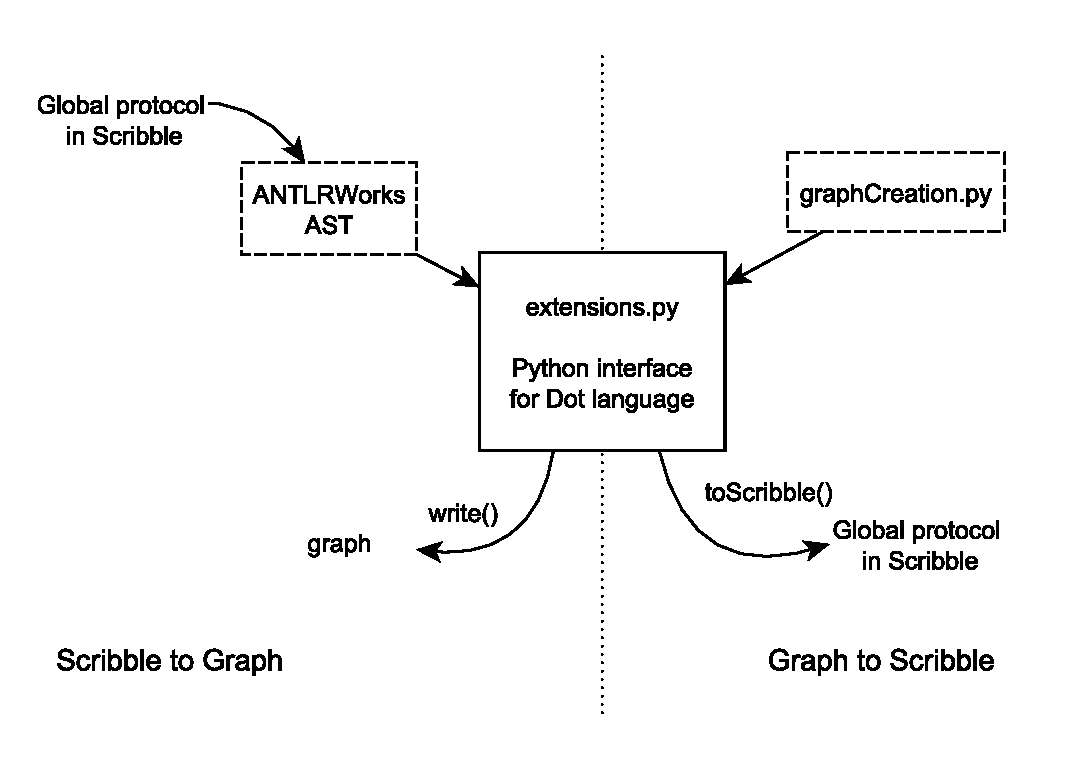
\includegraphics[scale=0.7]{structure}
\end{center}
\caption{General structure for the development}\label{fig:structure}
\end{figure}

Figure \ref{fig:structure} represents the general structure that supports our development. The central data structure of our correspondence between graph representations, following the design we have defined in chapter 2, and global protocols in Scribble, is a script describing the graph in the Dot language. We will introduce the Dot language in chapter 4. To write this script, we use a Python file that we have developed and called \emph{extensions}. This file indeed extends a Python library, which implements an interface for the Dot language, as we will explain later.

On one hand, we start with the Scribble protocol and parse it to obtain the script, and then from the script we print the graph. On the other hand, we start with the code of the script and print the protocol in Scribble. We explain in more details the structure in the following sections.



\section{From Scribble protocol to graph}
We begin with exposing how we manage from a global protocol in the Scribble language to obtain a graph. We chose to start with this way of the correspondence because the global protocol is already fixed by the research community, whereas the graphic objects were to define.

\subsection{Method}
\begin{figure}[h]
\begin{center}
\includegraphics[scale=0.7]{generalstructure}
\end{center}
\caption{Structure of the development}\label{fig:generalstructure}
\end{figure}

We can divide the work into two parts: (1) read the protocol and store the data, (2) while going through the collected data, create the graph. The first part was done within ANTLRWorks and the second in an Eclipse environment, as represented in Figure \ref{fig:generalstructure}. 

Given a global protocol in Scribble, the first issue for our program is to read it. The corresponding step in our development is to define a grammar for the global protocol in Scribble. This grammar allows decomposing a protocol into several predefined structures by defining lexer rules and parser rules. For each of these structures, we build a part of a tree with the essential information extracted from the protocol.

While parsing a Scribble global protocol, we build an abstract syntax tree. This will later be used to create the graphical representation of the protocol. An abstract syntax tree is, as its name states it, a data structure created from the protocol, in order to reuse the data of the protocol which were read.

Once an abstract syntax tree is built from the parsing of the protocol, it is possible to walk through it. To do this, ANTLRWorks allows defining a grammar for trees, which is: for each sub-structure of the tree we can state some code in Python. As well as providing an easy tool to build grammars, ANTLRWorks can generate Python files that can be reused and modified in a larger project. 

Figure \ref{fig:zoomstructure} represents the structure of the development with some details that we explain next.

\begin{figure}[h]
\begin{center}
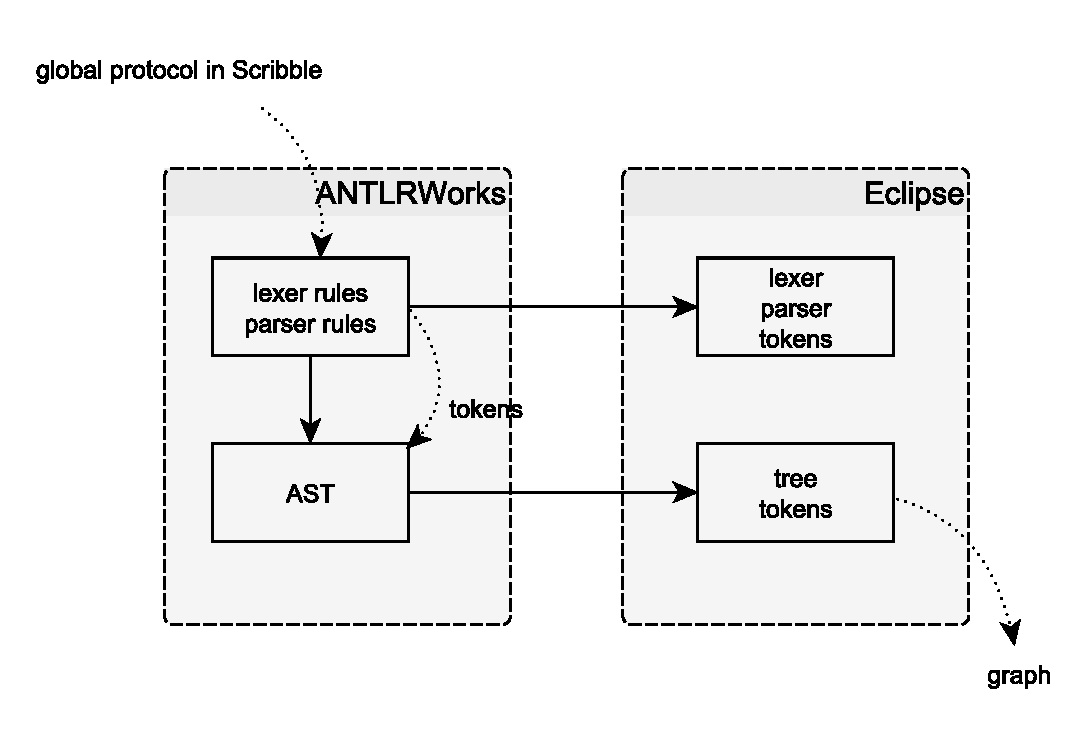
\includegraphics[scale=0.7]{zoomstructure}
\end{center}
\caption{Details of the structure for the development}\label{fig:zoomstructure}
\end{figure}

\subsection{ANTLRWorks}
Following this method, we have developed a lexer and a parser using the ANTLRWorks tool. ANTLRWorks is a grammar development environment for ANTLR v3 grammars. It combines a grammar-aware editor with an interpreter for rapid prototyping and a language-agnostic debugger for isolating grammar errors. ANTLRWorks helps eliminate grammar nondeterminisms by highlighting nondeterministic paths in the syntax diagram associated with a grammar.

\subsection{Lexer, Parser}
The lexer and parser are defined with some rules. Lexer rules define the tokens used to identify parts of the protocol during the reading, whereas a parser rule states how a structure of the protocol will be stored in the abstract syntax tree, as explained next.

The parsing rules we developed follow the grammar underlying the Scribble language, as specified in \cite{scribblelanguage}. We define tokens to be subtrees' roots. The grammar states the way it is built. One significant feature of ANTLR is the rewrite rule: it allows creating our own tokens to structure the tree rather than using the ones read by the lexer.

\begin{figure}[h]
\begin{center}
\includegraphics{choicerule2}
~~\\
\includegraphics[scale=0.5]{choicerule}
\end{center}
\caption{An example of a parser rule and its diagram: the choice case}
\label{fig:choicerule}
\end{figure}
For each activities (message, recursion, choice, etc.), there is a node in the corresponding abstract syntax tree. Its children are the added information. For instance a choice node will have a role as its first son, corresponding to the role that makes the choice, and then as many other sons as there are alternatives, as represented in Figure \ref{fig:choicerule}. An alternative will be represented as a block. The protocol body is also a block. A block is a node whose son is an activity list. The latter is also a node whose sons are consecutives activities, in the same order as defined in the protocol. These different levels of syntax allow avoiding grammar nondeterminism.


~~\\

Therefore given a Scribble global protocol in input of the program we obtain, after parsing and walking through the abstract syntax tree, the graph representation of the protocol. More details will follow in the next chapter.

\section{From graph to Scribble protocol}
\begin{figure}[h]
\begin{center}
\includegraphics[scale=0.7]{graphtoscr}
\end{center}
\caption{Representation of the development}
\label{fig:graphtoscr}
\end{figure}

We have described in the previous section how we have carried out the generation of a graph from the global protocol, we will now explain the other way round. It is indeed often easier for an engineer to draw a graph rather than to write the code for a protocol. Moreover discussing about a graph is more interactive for designing rather than commenting a code. That is why we want to be able to build first the graph and obtain from it the global protocol.

The first step is to create the graph we want to start from. For this purpose, we do not use any particular software but the same graphic objects we have developed in Python to generate the graph. While creating the graph, we store added pieces of information, which are its name and the concerned roles. It will be useful to write the protocol declaration as represented in Figure \ref{fig:graphtoscr}.

The next step to obtain the global protocol is to walk through the created graph and write the protocol with the information stored in the nodes. From one node to the next one, we walk through the whole graph to retrieve all necessary pieces of information. We begin with the first node of the graph, which is the start node. Therefore we are able to print the global protocol in Scribble. 




\chapter{Details of the implementation}

Along with the development we kept on improving our graph notations in order to obtain the ones presented in chapter 2. Implementing was indeed useful to refine or improve our first thoughts. We present here some details about the implementation: the issues faced, the structure of the code, and the choices made for the design. Most of the work exposed hereunder was done in an Eclipse environment as it allows for more flexibility in the code. 

\section{Structure of the code}

\begin{figure}[h]
\begin{center}
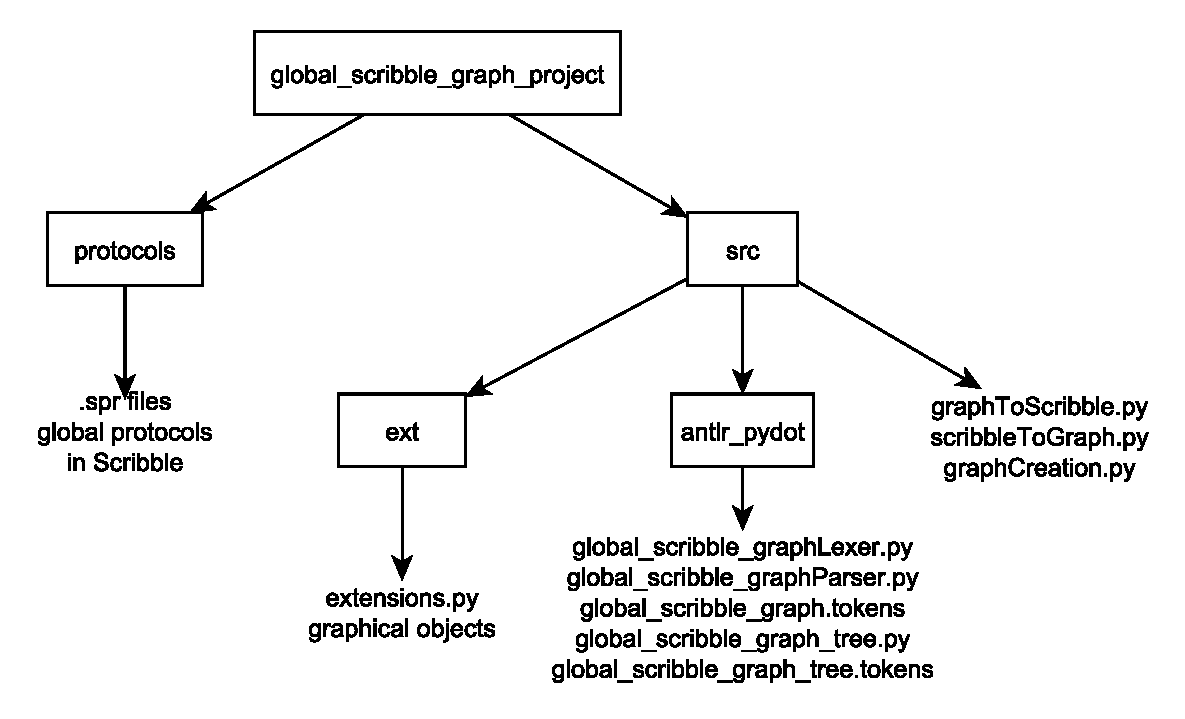
\includegraphics[scale=0.7]{project_organisation}
\end{center}
\caption{Overview of the project}\label{fig:project}
\end{figure}

We present in Figure\ref{fig:project} the project that we developed in Python in an Eclipse environment. We called our project \emph{global\_scribble\_graph\_project}. We have defined two separate packages:
\begin{itemize}
\item Protocols: it contains all the example of protocols we used during the development.
\item Source: it contains a sub-package with all the files generated with ANTLRWorks, another sub-package ext with the extensions of Pydot (This file defines the graphical objects we use in our project), and also other Python files: the main method for both ways and a file to specify graphs in Python.
\end{itemize}

We present in the following sections the details of the implementation of this project.

\section{The Python library: an extension of pydot}
The choice of developing our own graphical notations implies to create some graphical objects. We have chosen to develop the software in Python as it is the language already used in the research group. 



\subsection{Pydot}
In the literature there are several libraries for graph development. We have decided to use pydot, a Python interface to Graphviz's Dot language \cite{pydot}. 

Graphviz is an open source graph visualization software \cite{graphviz}. The Graphviz layout programs take descriptions of graphs in a simple text language, called Dot, and make diagrams in useful formats, such as images and SVG for web pages, PDF or Postscript for inclusion in other documents; or display in an interactive graph browser. (Graphviz also supports GXL, an XML dialect.)  Graphviz has many useful features for concrete diagrams, such as options for colors, fonts, tabular node layouts, line styles, hyperlinks, roll and custom shapes. The algorithm underlying the construction of a graph in Dot language is based on assigning nodes to discrete ranks and ordering nodes within ranks. 

Pydot allows easily creating both directed and non-directed graphs from Python. Currently all attributes implemented in the Dot language are supported (up to Graphviz 2.26.3). As well as downloading the pydot package, it is needed to download also graphviz and pyparsing in order to use it, as explains in Appendix with more details.

\subsection{Extensions}
\begin{figure}[h]
\begin{center}
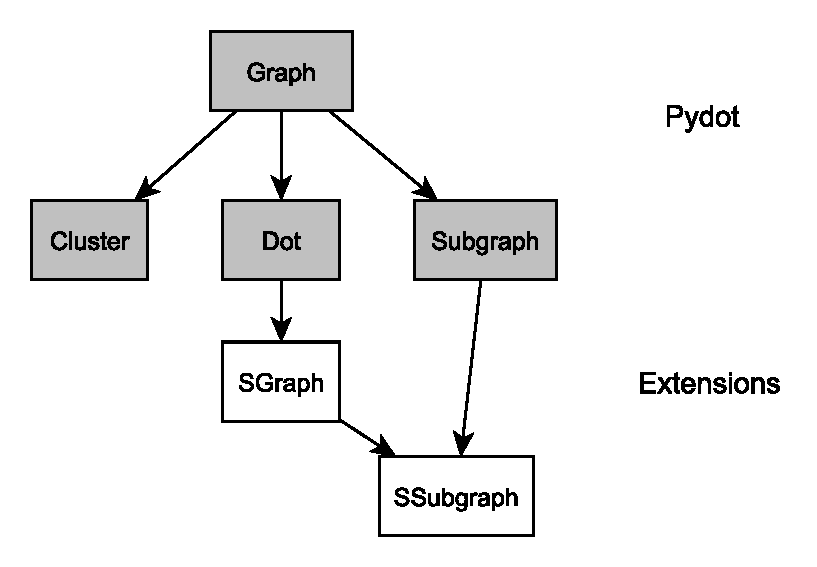
\includegraphics[scale=0.7]{graph_organisation}
\end{center}
\caption{Class diagram for graphs}
\label{fig:graph_organisation}
\end{figure}
From this existing library, we extended the code in order to create our own graphic objects: SNode, SEdge, SGraph, SSubgraph - S stands for Scribble. These objects inherit from the pydot objects Node, Edge, Dot, Subgraph, as presented in Figures \ref{fig:graph_organisation} and \ref{fig:node_organisation} and are designed to have the desired features. The SNode class has several derived class, corresponding to each type of nodes we expect, i.e. Start, Message, Choice, etc. As an example, we give here the code to define a Join node, as deriving from the SNode class:
\begin{SJLISTING}
class Join(SNode):
    
    def __init__(self, name = '', label = "|", style = 'bold', shape = 'diamond', obj_dict = None, **attrs):
        pydot.Node.__init__(self, name = name, label = label, style = style, shape = shape, 
				obj_dict = obj_dict, **attrs)
        
        if obj_dict is None:
            self.obj_dict['activity']='join'
\end{SJLISTING}

We also develop some new methods to deal with the operation we need, as explained in the following sections, or change some existing method.\\
For instance we add a method to obtain an edge from its source node:
\begin{SJLISTING}
    def get_edge_src(self, src):
        """Get the list of Edge instances which source is src.
        """
        edge_objs = list()
                           
        for edge, obj_dict_list in self.obj_dict['edges'].iteritems():
            if edge[0] == src:
                edge_objs.extend( [ SEdge( obj_dict = obj_d ) for obj_d in obj_dict_list ] )
        
        return edge_objs
\end{SJLISTING}
We change for example the method to add a node in a graph:
\begin{SJLISTING}
    def add_Snode(self,snode):
        """Adds a SNode object to the graph and store the roles.

        It takes a node object as its only argument and returns
        None.
        """
        if isinstance(snode, Message):

            self.add_role(snode.get_role1())
            self.add_role(snode.get_role2())
            
        if isinstance(snode, Choice):
            self.add_role(snode.get_role())
        
        self.add_node(snode)
\end{SJLISTING} 

We used this adapted library to deal with graphical objects in the development of the correspondence between the global protocol and the representation.

\begin{figure}[h]
\begin{center}
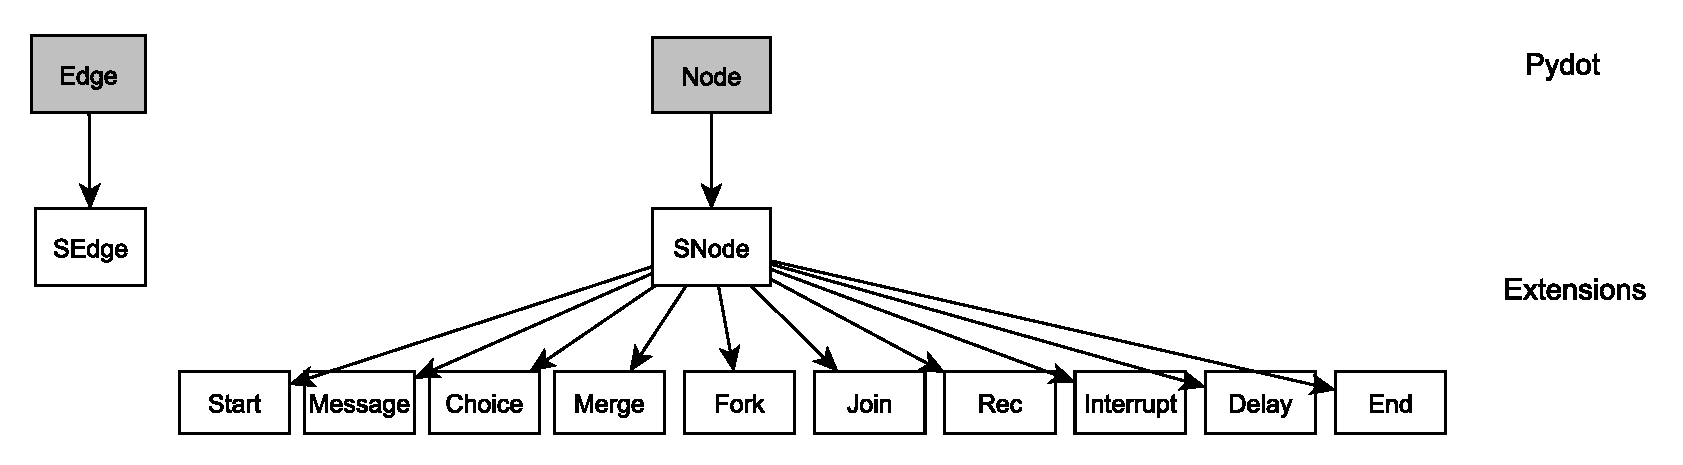
\includegraphics[scale=0.7]{node_organisation}
\end{center}
\caption{Class diagram for edges and nodes}
\label{fig:node_organisation}
\end{figure}


\section{From Scribble to graph}

\subsection{Main method}

Our code is based on the Python files generated with ANTLRWorks: the lexer, the parser and the tree. We use methods, predefined with the ANTLR tool, to write the main method: first we prepare the tree from the input with the lexer and the parser, and then we obtain a stream of all the nodes in a depth-first search way and execute the code associated with them. The processus is described in Figure \ref{fig:scrtograph}.

\begin{figure}[h]
\begin{center}
\includegraphics[scale=0.65]{scrtograph}
\end{center}
\caption{Implementation's structure from Scribble to graph}
\label{fig:scrtograph}
\end{figure}

As a result, walking through all the nodes of the abstract syntax tree allows creating all the nodes and edges needed for the graph. The last step consists in printing the graph. This method is defined in the pydot library: from the Python code it generates a script in the Dot language which in turn can be executed to produce the graph.

\begin{figure}[h]
\begin{center}
\includegraphics[scale=0.72]{mainmethod}
\end{center}
\caption{Code of the main method}
\label{fig:mainmethod}
\end{figure}


\subsection{Choices and assumptions}
We first give as an example the case of a simple interaction: \\
\texttt{msg = extensions.Message( nodeName, Message5.getChild(1).getText(), \\ Message5.getChild(2).getText(), msgLabel, timeLabel)\\
graph.add\_Snode(msg)}

When we meet a node Message, we program to create a graphic object Message (derived from SNode) with attributes Sender, Receiver, MessageLabel and TimeLabel, that are the ones stated in the leaves of the node Message. For this purpose we use the predefined methods \texttt{getChild()} and \texttt{getText()}.

In the same way we build nodes for the other activities. For choice (respectively fork) nodes, after creating them we proceed with the alternative blocks which number is evaluated with the methods \texttt{getChildCount()}. In the case where there is no recursion inside the branches (respectively threads), we also create a merge (respectively join) node to close the choice (respectively parallel) section. This part of code may evolve when Scribble will support merge and join constructs, as well as explicit end. For the recursion, we assume that each recursion label is unique, as it will be the name of the node.

It is worth noting that each node should have a different name. To solve this issue we associate to the graph a counter that generates integers to name the nodes. 

The execution of each activity returns two nodes the first one and last one: for instance, for a message both are the created node Message and for a choice it is the choice node and the merge node. Also an activity list, as well as a block, take in argument the previous node and return its last one in order to be able to build transitions between blocks. Then for the edges of the graph, we build them in the activity list section from one son to the next one, retrieving the nodes from the activities.\\
\texttt{
begin, end = self.activity(graph)\\
\# action start\\ 
\# at this point, we make the connection between the previous node (start) and the first activity and within the activities in the list\\
 edge = extensions.SEdge(currentNode, begin)\\
 graph.add\_Sedge(edge)\\
 currentNode = end\\
\# action end}

\section{From graph to Scribble}

\subsection{Creation of the graph}
For the creation of the graph, we use the graphic library described in a previous section: the extension of pydot. It is indeed the central part of our correspondence between graphs and Scribble protocols, as presented in Figure \ref{fig:structure}. It allows creating graph, nodes, edges and subgraphs. We can also create edges to link these objects together and specify, if needed, the headport and tailport of the edge to obtain the expected visualization. The call to the method \texttt{graph.print()} generates the given graph. The development of this way of the correspondence brings us to continue extending the library. 

\subsection{Generation of the protocol}
For this purpose, we have created a method called \texttt{toScribble()}, defined in the classes SGraph and SNode, and implemented in SGraph and the derived classes of SNode. The call of this method for a SNode prints the protocol concerning this node and also obtains the next node in the graph to go ahead. Therefore we develop also a method \texttt{next\_nodes()} as follows:
\begin{SJLISTING}
def next_nodes(self, graph):
        edges =graph.get_edge_src(self.get_name())
        names =[]
        next_nodes = []
        for e in edges:
            names = names+[e.get_destination()]
        for n in names:
            next_nodes = next_nodes + graph.get_Snode(n)
        return next_nodes
\end{SJLISTING}

For the parallel case, we first deal with the inside blocks from the fork node until the join node, then we continue with the node after the join one. It works in the same way for the choice case. However, we have to pay attention whether there is a join node (respectively a merge node) or not, to know when to stops. That is why the \texttt{toScribble()} method returns both the code and the end node of the constructs if there is one, for instance it could be a join node, and also why we use a flag to mark if one thread does not finish because of a recursion. The detail of the code is in Appendix.

We assume that after a message, recursion or interrupt node there is only one node. For the recursion - continue construct, we set a flag in the recursion node the first time we reach it and change it the second time in order to distinguish between the two syntax.

The method also manages to indent the protocol and print it in a pretty way in order to get a readable global protocol. 
~~\\
~~\\

To conclude, we now have a correspondence between global protocols in Scribble and a graph representation. It means for the following that all work done to extend the graph representation should also extend Scribble protocols and the underlying theory, and vice-versa. We will apply this on an extension handling with a notion of time.




\chapter{Towards graphs with time}

\section{General presentation}
As we aim at modelling real situations where several processes are interacting, such as the use case from the Ocean Observatories Initiative, we have to handle a notion of time, which is an important feature of physical systems. That is why we explore now how to extend our graph with time. This chapter introduces the notations, whereas the next one presents the theory underlying our model.

\subsection{Useful definitions}
We first give here some definitions from the Oxford dictionary in order to clarify terms we will use in this chapter.

\textbf{Delay} A period of time by which something is late or postponed.

\textbf{Timer} An automatic mechanism for activating a device at a preset time.

\textbf{Timeout} A cancellation or cessation that automatically occurs when a predefined interval of time has passed without a certain event occurring.


\subsection{Motivations}
Our current model allows representing complex interactions among several processes such as concurrency, recursion and branching. Theoretically there should be neither errors nor deadlocks. However, for critical software for instance, it sounds more realistic to have timeouts for each interaction. It allows indeed to avoid situation where a process is stuck waiting for a message. This is major issue for distributed systems.

Furthermore, to be able to handle time constraints in a scenario extends the expressiveness of our model: that is not only timeouts, but also several types of time constraints like delays. Time as a physical parameter has indeed an influence in most of real use cases.

Therefore we aim at introducing continuous time in our protocols by adding a set of clocks. To achieve this, we first focus on the graphical representation to figure out how to express time with our graph notations, and also on Scribble, as it corresponds to the graph. A second step is to define the theory underlying this notion of time. For this purpose we want to extend our previous syntax for generalised global protocols to continue supporting the extended Scribble language. Finally we will adapt our previous implementation work to encompass all these changes and guarantee the equivalence we have established between graphs and Scribble global protocols.


\section{Design}
We introduce in this section the design we have chosen to represent timeouts, delays and other time constraints. 

\subsection{General example}
To illustrate our motivations, we look at a variation of the example from the Ocean Observatories Initiative mentioned at the beginning of this report. Our goal does indeed remain to develop a graphical representation that expresses as precisely as possible a global scenario. Therefore we begin with defining which features we want to express on the graph and how to represent them.

\begin{figure}[p]
\begin{center}
\includegraphics[scale=0.44]{DataAcquisitionExample}
\end{center}
\caption{A variation of Use Case "Acquire Data from Instrument"}
\label{ooiwithdelay}
\end{figure}

The graph in Figure \ref{ooiwithdelay} presents three main differences against the first one: (1) the \emph{within} statement inside the message boxes, (2) the clock node, and (3) the constraints on arrows.

The \emph{within} statement provides a notion of timeout on interactions. For instance, 
\begin{center}
\fbox{\begin{minipage}{4cm}
\begin{center}
A $\rightarrow$ I: PushMode\\
within 1s
\end{center}
\end{minipage}
}
\end{center}
means that I should receive the message \emph{PushMode} at most one unit of time after A has sent it.

The clock node represents a notion of delay. It can be expressed either as relative time or as absolute time. A clock with the label t + 3min means that the next interaction will happen in three minutes with respect to the clock t. While a clock with the label t = 5s means that the next interaction will happen when the clock t will indicate 5s.

The labels on the arrows refer to the different time constraints we require. It also specifies clocks to be reset with a label like t1 = 0s. Therefore clocks encompass the notion of timer. It is possible to define several constraints on one arrow.

It is possible to define as many clocks as needed. In our example, we use six clocks. We assume that at the beginning all the clocks are set to 0.

\subsection{A new node: Delay}
\begin{figure}[h]
\begin{center}
\includegraphics[height=10cm]{Delay}\caption{Representation of the delay}
\label{fig:Delay}
\end{center}
\end{figure}
We study here a protocol containing a delay specification. Its name is \emph{FirstDelay} and it involves two roles: A and I. The protocol specifies that I sends a message to A, and then there is a delay before A sends to I the message \emph{ConfigPush}. A has indeed to wait for three seconds before continuing with the next interaction.\\
The graph representing this protocol, Figure \ref{fig:Delay}, is composed of one new node:
\begin{itemize}
\item The delay node: a clock with the time to wait on the top right.
\end{itemize}
The node states the delay to be waited for. t represents the current time on clock t. Therefore t + 3s means that if the time on clock t states 5s, we have to wait until t = 8s. In constrast to other time constraints, which are represented on the arrows, we have chosen to represent delay with a node. In a sense it is indeed an activity with an action, i.e. waiting.

The program in Scribble for this protocol is as follows:
\begin{center}
\begin{tabular}{ll}
\begin{SJLISTING}
global protocol FirstDelay ( role A, role I) {
	NotSupported from I to A within 1s;
	wait for t + 3s
	ConfigPush from A to I within 1s;
}
\end{SJLISTING}
& \\
\end{tabular}
\end{center}

\section{Extension of the Scribble language}
To conform the notations we have defined for graphs, we extend the Scribble language. We use the same syntax notations as the one introduced in a previous section to declare the grammar of the language. 
\begin{center}
\begin{tabular}{rcl}
global-protocol-body & ::= & global-interaction-block \\
global-interaction-block & ::= & \{ global-interaction-sequence \}  \\
global-interaction-sequence & ::= & ( global-interaction )*  \\
global-interaction & ::= & [ time-constraints ] message  \\
 & | & [ time-constraints ] choice  \\
 & | & [ time-constraints ] parallel \\
 & | & [ time-constraints ] recursion \\  
 & | & [ time-constraints ] continue  \\
 & | & [ time-constraints ] delay\\
message & ::= & ( message-signature | identifier)  \texttt{from} role-name  \texttt{to} role-name  \texttt{within} time;\\
delay & ::= &  \texttt{wait for} time-identifier symbol time ;\\
 & | &  \texttt{wait for} time-identifier \texttt{is} time ; \\
time-constraints & ::= &  constraint (\texttt{and} constraint )* \\
constraint & ::= &  time-identifier  \texttt{after} time   \\
 & | &  time-identifier \texttt{before} time \\
 & | &  time-identifier \texttt{is} time \\
time-identifier & ::= &  identifier \\
time & ::= &   ( digit  )* identifier \\
symbol &  ::= &  ( ‘+’ | ’*’ )\\
\end{tabular}
\end{center}
There are three major differences as for the graph representation: (1) the time constraints, (2) the delay, and (3) the \emph{within} statement.

Time constraints can be defined before each activity as an optional element. It represents constraints that a user writes on the arrows of the graph representing the global protocol. We assume that there is no constraint on the last arrow pointing at the end node. Time constraints consist of  one or more constraints. A date represents an absolute time, for instance 10h.

Delay is a new activity that consists in waiting for a specific time: it could be a relative time, for instance t+3h, or an absolute time, for instance t= 10h. It corresponds to the clock notation on the graph.

The \emph{within} statement has the same meaning as the one define for the graph, for instance within 2s.

Therefore this language clearly match the notations we have introduced for graphs: it is now possible to obtain the equivalence between Scribble global protocols and graphs again.

\section{Implementation}
In order for our implementation to remain accurate with this extension, we extend the work previously done. It consists in three main changes:
\begin{itemize}
\item We extend the grammar in ANTLR to support the new Scribble grammar.
\item We create a new object node, called Delay, to correspond to the \emph{wait for} statement. It derives from the class SNode and has the symbol of a clock.
\item We add a new way to define an edge by specifying a time constraint besides the existing features with the method \texttt{graph.add\_Sedge\_with\_label(edge,label)}.
\end{itemize}
Based on these changes, our implementation handles now the cases of timed global protocols and timed graphs.




\chapter{Timed global protocol}
As we have now set our graphical notations, we focus on the way to express them theoretically. We will first present some results one can find in the literature about time.

\section{Related work}
We discuss here some related issues, that is in which way a notion of time was introduced in several contexts: in contract formalism, in Pi-calculus, in colored Petri-nets and in automata.

\subsection{Contract formalism}
We first look at contract formalism. We will not give much details as we can find a survey about the topic in \cite{hvitved12phd}. In this thesis, the author defines the contract formalisation as "mathematical models and domain-specific languages for specifying and reasoning about contract". Furthermore, "a contract is a legally binding agreement between two or more parties, and a formalisation is an unambiguous, machine-interpretable representation". In practice, a contract will describe the actions that participants agree to perform.

Most of the contracts are based on a notion of time and in particular of deadline. To handle with this issue, several approaches were developed: (1) logic-based, (2) event-condition-action based, (3) trace-based. Two kind of temporal constraints can be distinguished: the absolute ones and the relative ones.

In \cite{hvitved12jlap}, they propose a trace-based approach. The main idea is that actions of one trace are time stamped and each obligation must have a deadline. Then "all deadlines that occur in clauses are relative to unspecified reference points which are given by the starting time of the specification and by the time of event occurrences. Thus, these relative deadlines are lifted to absolute deadlines when the CSL (Contract Specification Language) specification is executed." An obligation clause looks like:
\begin{center}
<p> k(x) where e due after $n_{1}$ within $n_{2}$ remaining z then c
\end{center}
where p are the parties, k a type, x binds to e an expression,$ n_{i}$ are times that binds z and c is a clause.

To specify an alternative continuation branch, which becomes active if the deadline passes, they define external choices.

This formalisation can inspire us a way to include time in global protocols. We could define deadlines (after $t_{1}$ before $t_{2}$) and associate them to blocks of activities inside a protocol. It would mean: this block of activity has to be done within the period defined by the deadline. We have tried to include this feature in our work. However it is not easily representable in a graph in an intuitive way, so we will not consider this possibility in our later work.


\subsection{Timer}
We present here an approach to introduce timer in Pi-calculus. In \cite{berger2007timed,berger2002towards} they introduce a timer to offer channel-based distributed liveness, ie a timer is a converter from (potential) non-terminating rule to terminating channels. The definition for processes is extended with:
\begin{center}
$timer^{t}\langle$ a($\tilde{x}$).P,Q$\rangle $, with t an integer such that t>0
\end{center}
It means that after t  steps it turns into process Q, unless it has been stopped, i.e. a message has been received by a timer at a.

The flow of time is communicated at each step in the computation by a time stepper function $\Phi$, which acts on processes. It models the implicit broadcast of time passing.
\begin{center}
\begin{tabular}{lrcl}
 &$\Phi ( timer^{t+1}\langle \PP, Q \rangle)$ & = & $timer^{t}\langle \PP, Q \rangle$ \\
 &$\Phi ( timer^{1}\langle \PP, Q \rangle)$ & = & Q \\
 &$\Phi (\PP \| Q)$ & = & $\Phi (\PP) \| \Phi (Q) $\\
 &$\Phi ( \nuc{\Ia}{\PP} )$ & = & $\nuc{\Ia}{ \Phi (\PP)}$\\
otherwise& $\Phi (\PP) $ & = & \PP\\
\end{tabular}
\end{center}

This timer aims at an efficient implementation of periodic behaviour and error recovery. It is indeed possible to extend the calculus to define a recovery mechanism.

In the same way, in \cite{ciobanu2006timers} they define timed distributed Pi-calculus  and introduce time constraints by considering timeout timers for channels. The possible communications are performed at each tick of a universal clock. Active channels are those which could be involved in these communications. The time-stepping function affects the active channels which do not communicate at that tick; the timers of the affected channels are decreased by one unit of time. Furthermore they guarantee some properties like time determinism, maximal progress and time continuity.

Finally, in \cite{lee2002modeling} they develop an extended algebra allowing both time values as well as names to be transmitted between processes, called the $\pi$RT-calculus. The new feature of the model is based on timeouts and on the distinction between when an action is possible (enabled) and when an action actually occurs (fires) since they might be delay between these two states. Therefore they propose a timed labelled transition system. 


\subsection{Timed Colored Petri-Nets}
We can find lots of work on Petri-nets in the literature as they are appropriate for the modelling of distributed systems, since they allow for the representation of parallelism and synchronization (\cite{vanderaalst1992timed,desel1995free}).

In \cite{vanderaalst1992timed} they introduce timed colored Petri-nets. A colored Petri-net is one where tokens have a value, often referred to as 'colour'. Then each place has a type (a set of colours) and tokens in a place have a value (a colour) belonging to the corresponding type. As they aim at expressing quantitative temporal properties like deadlines, activity duration, response times and delays, they also add a notion of time. They attach a time-stamp to every token. This time-stamp indicates the time a token becomes available. The enabling time of a transition is the maximum time-stamp of the tokens to be consumed. The difference between the firing time and the time-stamp of such a produced token is called the firing delay. To describe time delays, they use intervals. It allows for the representation of time constraints.

In \cite{van1998application} Petri-nets are applied to workflow management with the introduction of a trigger for each transition. There are four types of triggering: time, message, user and automatic (the default one). The principle underpinning the trigger is that an external condition leads to the execution of an enabled task.



\subsection{Timed Automata}
We now expose the main principles of timed automata as introduced in \cite{alur1994theory,alur1999timed,bengtsson2004timed}. They aim at modelling the behaviour of real-time systems over time. The timed (finite) automata are defined to be a way to annotate state-transition graphs with timing constraints using finitely many real-valued clocks.

These automata are based on timed words which are obtained by coupling a real-valued time with each symbol in a word. Then, when an automaton makes a transition, the choice of the next state depends not only upon the input symbol, but also on the time of this input symbol relative to the times of the previously read symbols. For this purpose, they associate a finite set of (real-valued) clocks with each transition table. A clock can be set to zero simultaneously with any transition. At any instant, the reading of a clock equals the time elapsed since the last time was reset. With each transition, they associate a clock constraint, and require that the transition may be taken only if the current values of the clocks satisfy this constraint. Having multiple clocks allows multiple concurrent delays. The clocks of the automaton do not correspond to the local clocks of different components in a distributed system. They also assume that all the clocks increase at the uniform rate counting time with respect to a fixed global time frame.

They demonstrate in the paper how timed automata can capture several aspects of real-time systems: qualitative features such as liveness, fairness, and non-determinism; and quantitative features such as periodicity, bounded response, and timing delays. We will present some of these aspects in more details in the following sections.


\subsection{Timed Pi-calculus}
In \cite{saeedloei2008timed} they introduce clocks (or stopwatches) and two types of clock operations: clock resets and clock constraints in order to extend Pi-calculus with real-time. Then the future behaviour of a real-time system depends not only on the content of a receiving message, but also on the time-stamp of the message. In other words, the time-stamp of the arriving/sent message should satisfy certain time constraints specified by the system, for future transitions to take place. Therefore, there are two new variables: (1) the time-stamp of the message $t_{m}$, (2) the clock of the process which sends the message c. A message is then represented by $\langle m, t_{m}, c \rangle$. They assume that processes have access to countable set of clocks when they are needed and that all clocks advanced at the same rate.

The calculus is defined as follows:
\begin{center}
\begin{tabular}{rclr}
C & ::= & $Reset\ \|\ Constraint \ \|\ \epsilon$ & (Clock operations)\\
Reset & ::= & $(reset Clock) \ \|\ Constraint (reset Clock) $& \\
Constraint & ::= & ce $\sim$ 0 & \\ 
ce & ::= & $x + ce \ \|\ x - ce\ \|\ x $& \\
x & ::= &$ Numbe\ \| \ Clock$ & \\
tild & ::= &$ <\ \|\ >\ \|\ \le\ \|\ \ge\ \|\ =$ & \\
$\Pi$ & ::= & $ C\bar{x}\langle y, t_{y}, c \rangle\ \|\ Cx(\langle z,t_{z},c\rangle)\ \|\ C\tau\ \|\ [x=y]\pi\ \|\ Reset\ \|\ Constraint $& (Processes) \\
\end{tabular}
\end{center}


\subsection{Other work}
We can find several other pieces of work on the same topic in the literature. For instance, in \cite{maggi2011monitoring} they work on runtime verification framework based on linear temporal logic and colored automata. The framework continuously verifies compliance with respect to a predefined constraint model and is able to recover after the first constraint violation. We also mention here a timed session request defined in \cite{lopez2010towards}:
\begin{center}
\begin{tabular}{rlr}
P ::= & request a(k) during m  in P & Timed session request\\
 & $\|\ $ accept a(k) given c  in P& \\
 & ~~~ ... & \\
 & $\|\ $kill $c_{k}$ & Session abortion\\
\end{tabular}
\end{center}

Furthermore, we can find other extensions that use similar techniques, such as a theory of multiparty session types
with assertions based on symmetric sum types (\cite{henriksentrustworthy}) or the introduction of global assertion which specifies a session type with logical predicates (\cite{bocchi2010theory,bocchisafety}).

~~\\

Based on this analysis of previous work, we now present the theoretical part of this work. What is new in our extension is to introduce time for global protocols: both in the Scribble syntax and in global/local types.

\section{The syntax}
As we have fixed the notations concerning time for graphs and Scribble language, we now present the chosen syntax to support these notations. We propose new types for the theory to support the extended Scribble language. For this purpose, we adapt some work from \cite{alur1994theory,saeedloei2008timed} to our case.


\subsection{Primarily notations}
Before stating the protocols types, we introduce a few notations. The definition are similar to the ones for timed automata in \cite{alur1994theory}.

We first declare a set of clocks to express several time notions and constraints. For a set X of clock variables, the set $\Phi$(X) of clock constraints $\delta$ is defined inductively by:
\begin{center}
$\delta := x \le c ~|~ x \ge c ~|~ \neg \delta ~|~ \delta_{1} \wedge \delta_{2} ~|~ \epsilon$ 
\end{center}
where x is a clock in X and c is a constant in $\mathbb{Q}$.
We also introduce useful abbreviations:
\begin{center}
\begin{tabular}{rcl}
x = c& means& x $\le$ c and  x $\ge$ c\\
x < c& means& $\neg$ x $\ge$ c\\
x > c& means& $\neg$ x $\le$ c\\
\end{tabular}
\end{center}
Clock constraints that follow this syntax are well-formed constrainst. For instance $t_1 = 3 \wedge t_2 < 5$ is a well-formed clock constraint.

A clock interpretation v for a set X of clocks assigns a real value to each clock, i.e. it is a mapping from X to $\mathbb{R}$. At the beginning, all clocks are assigned to 0. Then the values change as time goes on, or clocks are reset to 0.



\subsection{As a generalised global type}
From the global point of view, the syntax is defined as follows:
\begin{center}
\begin{tabular}{rcll}
G & ::= & def $\tilde{\G}$ in x & Global type \\
$\G$ & ::= & x  = p $\rightarrow p' : l \langle \UT \rangle, \lambda_{O}, \delta_{O}, \lambda_{I}, \delta_{I} ;x' $ & Labelled messages\\
& | & x = x' | x'' & Fork\\
& | & x = x' + x'' & Choice\\
& | & x | x' = x'' & Join\\
& | & x + x' = x'' & Merge\\
& | & x = $\End$ & End\\
\UT & ::= &$ \langle G\rangle\ |\ \Bool\ |\ nat \ |\ \ldots\ $ & Sorts
\end{tabular}
\end{center}
The major difference against generalised global types defined in \cite{denielou2012multiparty} is the labelled message:\begin{center}
x  = p $\rightarrow p' : l \langle \UT \rangle, \lambda_{O}, \delta_{O}, \lambda_{I}, \delta_{I}$ ;x'
\end{center}
p and p' denote respectively the sending and receiving participants. U is the payload type of the message and l its label. 

Let C be a finite set of clocks. $\lambda_{O}, \lambda_{I}$ are included in C and denote the set of clocks to reset. O stands for output and I for input. This means that $\lambda_{O}$ denote the clocks to be reset during the output action, and $\lambda_{I}$ the clocks to be reset during the input action. $\delta_{O}, \delta_{I}$ are clock constraints over C. $\delta_{O}$ denote the constraint to satisfy to send the message and $\delta_{I}$ the one to satisfy to receive the message.

For instance we could have,
\begin{center}
x = A $\rightarrow$ B : TheMessage <bool> , \{$t_{x}\}, t > 3, \{t_1\}, t_{x}$ < 2  ;  x’ 
\end{center}
This means that to go from state x to state x', 
\begin{itemize}
\item A has to reset the clock $t_x$ while sending the message labelled \emph{TheMessage} and carrying a boolean to B if the condition t > 3 is satisfied.
\item B has to reset the clocks $t_1$ while receiving the message labelled \emph{TheMessage} and carrying a boolean from A if the condition $t_x$ < 2 is satisfied.
\end{itemize}
$t, t_x, t_1$ are clocks associated to the corresponding global protocol.

This interaction could be a part of this protocol:\\
\begin{tabular}{ll}
~&~\\
\begin{SJLISTING}
global protocol ExampleCFSM (role A, role B){
	t before 3s
	TheMessage from A to B within 2s;
	wait for t1 + 1s
}
\end{SJLISTING}
&\\
~&~\\
\end{tabular}\\
Figure \ref{fig:excfsm} represents the protocol.

\begin{figure}[h]
\begin{center}
\includegraphics[height=8cm]{ExampleCFSM}\caption{Example to illustrate the new syntax}\label{fig:excfsm}
\end{center}
\end{figure}


\subsection{As a local type}
In order for the local types syntax to correspond to the communicating finite states machines previously defined, we extend the local types syntax.
\begin{center}
\begin{tabular}{rcll}
T & ::= & def $\tilde{\T}$ in x & Local type \\
$\T$ & ::= & x  = !$\langle p,  l \langle \UT \rangle, \lambda, \delta \rangle.x' $ & Message sending\\
& | & x  = ?$\langle p,  l \langle \UT \rangle, \lambda, \delta \rangle.x' $ & Message receiving\\
& | & x = x' | x'' & Fork\\
& | & x = x' $\oplus$ x'' & Internal choice\\ 
& | & x = x' \& x'' & External choice\\
& | & x | x' = x'' & Join\\
& | & x + x' = x'' & Merge\\
& | & x = x' & Inaction\\
& | & x = $\End$ & End\\
\UT & ::= &$ \langle G\rangle\ |\ \Bool\ |\ nat \ |\ \ldots\ $ & Sorts
\end{tabular}
\end{center}
As for global types, the major differences against generalised global types defined in \cite{denielou2012multiparty} are the message sending and the message receiving:
\begin{center}
x  = !$\langle p,  l \langle \UT \rangle, \lambda, \delta \rangle.x' $\\
x  = ?$\langle p,  l \langle \UT \rangle, \lambda, \delta \rangle.x' $ 
\end{center}
p denotes respectively the receiving and sending participants. U is the payload type of the message and l its label. 

Let C be a finite set of clocks. $\lambda$ is included in C and denotes the set of clocks to reset during the action.  $\delta$ is a clock constraint over C to satisfy to respectively send the message and receive the message.

For instance our previous example will be written from the point of view of A like:
\begin{center}
x = !$\langle$ B, TheMessage <bool> , \{$t_{x}$\}, t > 3 $\rangle$. x’ 
\end{center}
and from the point of view of B like:
\begin{center}
x = ?$\langle$ A, TheMessage <bool> , \{$t_1\}, t_{x}$ < 2 $\rangle$.x’ 
\end{center}
This has the same meaning as the one explained before.



\subsection{As communicating finite state machines}
Let define now a communicating finite state machine to represent the local behaviour: (Q, K, $q_0$, A, C, T), where Q is a finite set of states, K a finite set of channels, $q_0$ a initial state, C a finite state of clocks and T a finite set of transitions. There is a transition for each interaction, ie a message receiving or a message sending. These transitions carry the time information as constraints and  clocks resetting, ie T is included in Q x ( K x \{!,?\} x A x $2^C$ x $\Phi$(C) ) x Q. It extends the communicating finite state machine exposed in a previous section.

For instance, the two ommunicating finite state machines corresponding to our previous example are in Figure \ref{fig:localA} and \ref{fig:localB}.
\begin{figure}[h]
\begin{center}
\includegraphics[scale=0.7]{localA}\caption{From the point of view of A}\label{fig:localA}
\includegraphics[scale=0.7]{localB}\caption{From the point of view of B}\label{fig:localB}
\end{center}
\end{figure}

As for timed automata,we are interested in timed words $(\sigma,\tau_O, \tau_I)$, where $\tau = \tau_{1}\tau_{2}...$ is a time sequence. We need to guarantee $\tau_{O_0} < \tau_{I_0} < \tau_{O_1} < \tau_{I_1} < \tau_{O_2}$ ... In our example, corresponding time sequences have only one character, as there is only one transition, for instance 3.2 and 4.5 work. In fact any real number strictly greater than three is possible for the first one and the second one should add to the first one no more than 2. The associated timed word is \emph{(TheMessage, 3.2, 4.5)}.

At time $\tau_{O_{i}}$, the transition $\langle x_{i-1}, k_i, !,l_i, \lambda_{O_i}, \delta_{O_i}, x_i \rangle$ is such that: 
\begin{itemize}
\item $( v_{I_{i-1}} + \tau_{O_i} - \tau_{I_{i-1}} )$ satisfies $\delta_{O_i}$ 
\item $v_i$ equals $[\lambda_{O_i}\rightarrow0]( v_{I_{i-1}} + \tau_{O_i} - \tau_{I_{i-1}} )$, which means that clocks in $\lambda_{O_i}$ are reset to 0. 
\end{itemize}
At time $\tau_{I_{i}}$, the transition $\langle x_{i-1}, k_i, ?,l_i, \lambda_{I_i}, \delta_{I_i}, x_i \rangle$ is such that: 
\begin{itemize}
\item $( v_{O_i} + \tau_{I_i} - \tau_{O_{i}} )$ satisfies $\delta_{I_i}$ 
\item $v_i$ equals $[\lambda_{I_i}\rightarrow0]( v_{O_i} + \tau_{I_i} - \tau_{O_{i}} )$, which means that clocks in $\lambda_{I_i}$ are reset to 0. 
\end{itemize}
 We used here some notations in \cite{alur1994theory}. In our example, $v_0$ maps $t, t_1$ to 0, $\tau_{O_0}$ and $\tau_{I_0}$ are 0 and $\tau_{O_1}$ is 3.2 and $\tau_{I_1}$ is 4.5. Then $v_{I_0} + \tau_{O_1} - \tau_{I_0}$ is 3.2 for every clocks. Therefore t > 3 is satisfied. In the same way, $v_{O_1} + \tau_{I_1} - \tau_{O_1}$ is 1.3 for $t_x$ (it has been previously reset) and 4.5 for the other clocks. So $t_{x}$ < 2 is also satisfied.
~~\\

Therefore, we have defined all the syntax we need to match the graphs we want to be able to declare. We will now expose in more details how to express some features relative to time with these new notations.


\section{Expressiveness of the syntax}
We present here some examples to demonstrate the expressiveness of the syntax we have developed. At the starting point, all clocks are set to 0. 

\subsection{Timeout for message passing}
We begin with a simple graph with three nodes: a start node, an end node and a message node as follows.

\begin{center}
\fbox{\begin{minipage}{7cm}
\begin{center}
U $\rightarrow$ A: PollMode < InstrumentId, int >\\
within 2s
\end{center}
\end{minipage}
}
\end{center}

The complete graph is in Figure \ref{fig:Msg}.
For this graph, the corresponding Scribble global protocol is:\\
\begin{tabular}{ll}
~&~\\
\begin{SJLISTING}
global protocol TestMessage (role A, role U) {
	PollMode(InstrumentId,int) from U to A within 2s;
}
\end{SJLISTING}
&\\
~&~\\
\end{tabular}\\
To support this protocol we define the global type as follows:\\
\begin{tabular}{lrl}
G = & def & x = U $\rightarrow$ A : PollMode <InstrumentId, int> , \{$t_{x}\}, \epsilon, \varnothing, t_{x}$ < 2  ;  x’\\
&& x’ = end\\
& in x&\\
\end{tabular}\\
This means that we associate a unique, fresh clock, called $t_x$, to this message interaction and this clock will ensure the timeout for the message passing. Indeed, when U sends the message \emph{PollMode}, U sets the clock $t_x$ to 0. As A has also access to this clock, A can check that she receives the message \emph{PollMode} with respect to the constraint $t_x$ < 2. It means that A will not continue with x' if the timeout $t_{x}$ is over. Therefore it garantees that the interaction is performed within two units of time and the whole structure models therefore the \emph{within} statement from the global protocol in Scribble.

We also have the local types in the same way:\\
\begin{tabular}{lrl}
$T_{U}$ = & def &  x  = !$\langle$ A, PollMode <InstrumentId, int>  ,\{$t_{x}\},\epsilon \rangle$ . x’\\
&& x’ = end\\
& in x&\\
\end{tabular}\\
\begin{tabular}{lrl}
$T_{A}$ = & def &  x  = ?$\langle$ U,PollMode <InstrumentId, int>  , $\varnothing, t_{x} < 2 \rangle$ . x’\\
&& x’ = end\\
& in x&\\
\end{tabular}\\

\subsection{Delay}
We now add a delay before sending the message. First we look at the case of absolute time. The corresponding Scribble global protocol is:\\
\begin{tabular}{ll}
~&~\\
\begin{SJLISTING}
global protocol TestAbsoluteDelay (role A, role U) {
	wait for t is 17 h
	PollMode(InstrumentId,int) from U to A within 2 s;
}
\end{SJLISTING}
&\\
~&~\\
\end{tabular}\\
Figure \ref{fig:ad} represents this protocol.

\begin{figure}[h]
\begin{center}
\includegraphics[height=8cm]{TestAbsoluteDelay}\caption{Representation of the case of an absolute delay}\label{fig:ad}
\end{center}
\end{figure}

To support this protocol we define the global type as follows:\\
\begin{tabular}{lrl}
G = & def & x = U $\rightarrow$ A : PollMode <InstrumentId, int> , \{$t_{x}\}, t=17, \varnothing, t_{x}$ < 2  ;  x’\\
&& x’ = end\\
& in x&\\
\end{tabular}\\
What is new from the previous example is the output constraint t = 17. This means that U has to wait for t to be 17h to be able to send the message \emph{PollMode}. Therefore it models a delay.

We also have the local types in the same way:\\
\begin{tabular}{lrl}
$T_{U}$ = & def &  x  = !$\langle$ A, PollMode <InstrumentId, int>  ,\{$t_{x}$\}, t=17 $\rangle$ . x’\\
&& x’ = end\\
& in x&\\
\end{tabular}\\
\begin{tabular}{lrl}
$T_{A}$ = & def &  x  = ?$\langle$ U,PollMode <InstrumentId, int>  , $\varnothing, t_{x}$ < 2 $\rangle$ . x’\\
&& x’ = end\\
& in x&\\
\end{tabular}\\
~~\\

We now look at the case of relative time. The corresponding Scribble global protocol is:\\
\begin{tabular}{ll}
~&~\\
\begin{SJLISTING}
global protocol TestRelativeDelay (role A, role U) {
	PollMode(InstrumentId,int) from U to A within 2s;
	wait for t + 3 h
	PollMode from A to I within 1s;
}
\end{SJLISTING}
&\\
~&~\\
\end{tabular}\\
Figure \ref{fig:rd} represents this protocol.

\begin{figure}[h]
\begin{center}
\includegraphics[height=10cm]{TestRelativeDelay}\caption{Representation of the case of a relative delay}\label{fig:rd}
\end{center}
\end{figure}

To support this protocol we define the global type as follows:\\
\begin{tabular}{lrl}
G = & def & x = U $\rightarrow$ A : PollMode <InstrumentId, int> , \{ $t_{x}\}, \epsilon, \{ t \}, t_{x} < 2$  ;  x’\\
&& x' = A $\rightarrow$ I : PollMode, \{ $t_{x'}\}, t=3, \varnothing, t_{x'}<1 \wedge t=3$  ;  x’'\\
&& x’' = end\\
& in x&\\
\end{tabular}\\
There are two differences against the previous example: (1) \{t\}, and (2) t=3. These mean that t has to be reset to 0 by A when receiving the first message. In this case t will play the role of a timer. Then A will have to check when t equals three hours. Only when this constraint will be also satisfied, A will be able to send the second message.

We also have the local types in the same way:\\
\begin{tabular}{lrl}
$T_{U}$ = & def &  x  = !$\langle$ A, PollMode <InstrumentId, int>  ,\{ $t_{x}$\}, $\epsilon \rangle$ . x’\\
&& x’ = end\\
& in x&\\
\end{tabular}\\
\begin{tabular}{lrl}
$T_{A}$ = & def &  x  = ?$\langle$ U,PollMode <InstrumentId, int>  , $\{ t \}, t_{x} < 2 \rangle$ . x’\\
&& x'  = !$\langle$ I, PollMode,\{ $t_{x'}$\}, $t=3 \rangle$ . x’'\\
&& x’' = end\\
& in x&\\
\end{tabular}\\
\begin{tabular}{lrl}
$T_{I}$ = & def &  x'  = ?$\langle$ A,PollMode, $\varnothing, t_{x'} < 1 \rangle$ . x’'\\
&& x’' = end\\
& in x'&\\
\end{tabular}\\

\subsection{Time constraints}
Finally we consider the case of a constraint on the arrow going to the Message box. The corresponding Scribble global protocol is:\\
\begin{tabular}{ll}
~&~\\
\begin{SJLISTING}
global protocol TestConstraint (role A, role U) {
	t before 4 min
	PollMode(InstrumentId,int) from U to A within 2 s;
}
\end{SJLISTING}
&\\
~&~\\
\end{tabular}\\
Figure \ref{fig:cons} represents this protocol.

\begin{figure}[h]
\begin{center}
\includegraphics[height=6cm]{TestConstraint}\caption{Representation of the case of a constraint}\label{fig:cons}
\end{center}
\end{figure}

To support this protocol we define the global type as follows:\\
\begin{tabular}{lrl}
G = & def & x = U $\rightarrow$ A : PollMode <InstrumentId, int> , \{$t_{x}$\}, t < 4, $\varnothing, t_{x}$ < 2  ;  x’\\
&& x’ = end\\
& in x&\\
\end{tabular}\\
What is new is t < 4. This means that the constraint t < 4 has to be satisfied in order for U to send the message \emph{PollMode}.

We also have the local types in the same way:\\
\begin{tabular}{lrl}
$T_{U}$ = & def &  x  = !$\langle$ A, PollMode <InstrumentId, int>  ,\{$t_{x}$\}, t < 4 $\rangle$ . x’\\
&& x’ = end\\
& in x&\\
\end{tabular}\\
\begin{tabular}{lrl}
$T_{A}$ = & def &  x  = ?$\langle$ U,PollMode <InstrumentId, int>  , $\varnothing, t_{x}$ < 2 $\rangle$ . x’\\
&& x’ = end\\
& in x&\\
\end{tabular}\\



\section{Results}

\subsection{Well-formedness}
Clocks constraints should be formed as stated in section 6.2.1. We suggest an additional condition that should be checked.

\textbf{Temporal satisfiability }\textit{ If $\delta$, the clock condition of a given transition, is satisfiable at some point, for each constraint $\delta$', appearing in a later transition, it is eventually possible to satisfy $\delta$'.}

To demonstrate the need of this additional condition, we consider the following example.\\
\begin{tabular}{ll}
~&~\\
\begin{SJLISTING}
global protocol TestTemporalSatisfiability (role A, role B, role C) {
	wait for t = 5s
	Msg1(no1) from A to B within 2 s;
	choice at B {
		t after 6s
		Msg2(no2) from B to C within 1s;
	} or {
		Msg3(no3) from B to C within 1s;
	}
}
\end{SJLISTING}
&\\
~&~\\
\end{tabular}\\
Figure \ref{fig:ts} represents this protocol.

\begin{figure}[h]
\begin{center}
\includegraphics[height=12cm]{TestTemporalSatisfiability}\caption{Example of temporal satisfiability}\label{fig:ts}
\end{center}
\end{figure}

To support this protocol we define the global type as follows:\\
\begin{tabular}{lrl}
G = & def & $x_0$ = A $\rightarrow$ B : Msg1 <nat> , \{$t_{x_{0}}$\}, t = 5, $\varnothing, t_{x_0}$ < 2  ;  $x_1$\\
&& $x_1$ = $x_2$ + $x_3$ \\
&& $x_2$ = B $\rightarrow$ C : Msg2 <nat> , \{$t_{x_2}$\}, t < 6, $\varnothing, t_{x_2}$ < 1  ;  $x_4$\\
&& $x_3$ = B $\rightarrow$ C : Msg3 <nat> , \{$t_{x_3}$\}, $\epsilon$, $\varnothing, t_{x_3}$ < 1  ;  $x_5$\\
&& $x_4$ + $x_5$ = $x_6$ \\
&& $x_6$ = end\\
& in $x_0$ &\\
\end{tabular}\\
This means that when A send the message \emph{Msg1} to B, t equals five seconds. Then the message should be received within two seconds. Therefore if the condition $\delta$ = $t_{x_0}$ < 2 is satisfied, this means also that t < 7 is satisfied. In this case the condition $\delta$' = t > 6 can be satisfied at some point: either it is already satisfied because we could have 6 < t < 7, or it is not yet satisfied, but will eventually be satisfied when time goes on. The latter case could be assimilate to a delay, but it is not exactly the same. In the case of a delay, we know exactly the time when the delay has been achieved, whereas in this case, the message \emph{Msg2} can be sent whenever t is greater than six seconds. Therefore this example satisfies the temporal satisfiability condition.

On the other hand, if we consider the following global protocol in Scribble:\\
\begin{tabular}{ll}
~&~\\
\begin{SJLISTING}
global protocol TestTemporalSatisfiability (role A, role B, role C) {
	wait for t = 5s
	Msg1(no1) from A to B within 2 s;
	choice at B {
		t before 6s
		Msg2(no2) from B to C within 1s;
	} or {
		t after 6s
		Msg3(no3) from B to C within 1s;
	} or {
		Msg4(no4) from B to C within 1s;
	}
}
\end{SJLISTING}
&\\
~&~\\
\end{tabular}\\
we do not verify the temporal satisfiability condition, as there is the case when $\delta$ = $t_{x_0}$ < 2 is satisfied, and also t < 7, but $\delta$' = t < 6 is not satisfiable: for instance when t = 6.5 after the receiving of the message \emph{Msg1}. Such a situation means that the choice could be done only by temporal conditions, as it is not the case in our model. We state that the choice is done by a participant and all timed branches should be enabled at some point.

~~\\

We conjecture that a global type G = def $\tilde{\G}$ in $x_{0}$ is \textit{well-formed}, if it satisfies the sanity, local choice, linearity conditions\footnote{These conditions are defined in \cite{denielou2012multiparty}} and clock constraints the temporal satisfiability conditions. It is worth noting, that we may revise the local choice condition for global protocols in order to include the case when the choice only depends on time conditions.


\subsection{Projection}
The projection from a well-formed global protocol to local protocols, written G$\upharpoonright$ p, is straightforward from the syntax. We give here the algorithm:
\begin{center}
\begin{tabular}{rcl}
def $\tilde{\G}$ in x $\upharpoonright$ p & = & def $\tilde{\G}\upharpoonright_{\tilde{\G}}$ p in x \\
x  = p $\rightarrow p' : l \langle \UT \rangle, \lambda_{O}, \delta_{O}, \lambda_{I}, \delta_{I} ;x' \upharpoonright_{\tilde{\G}}$ p & = &  x  = !$\langle p',  l \langle \UT \rangle, \lambda_{O}, \delta_{O} \rangle.x' $ \\
x  = p $\rightarrow p' : l \langle \UT \rangle, \lambda_{O}, \delta_{O}, \lambda_{I}, \delta_{I} ;x' \upharpoonright_{\tilde{\G}}$ p' & = &  x  = ?$\langle p,  l \langle \UT \rangle, \lambda_{I}, \delta_{I} \rangle.x' $ \\
x  = p $\rightarrow p' : l \langle \UT \rangle, \lambda_{O}, \delta_{O}, \lambda_{I}, \delta_{I} ;x' \upharpoonright_{\tilde{\G}}$ p'' & = &  x = x' (p'' $\notin$ \{p,p'\})\\
x = x' | x'' $\upharpoonright_{\tilde{\G}}$ p & = &  x = x' | x''\\
x = x' + x'' $\upharpoonright_{\tilde{\G}}$ p & = & x = x' $\oplus$ x'' (if p = ASend($\tilde{\G}$)(x))\\
x = x' + x'' $\upharpoonright_{\tilde{\G}}$ p & = & x = x' \& x'' (otherwise)\\
x | x' = x'' $\upharpoonright_{\tilde{\G}}$ p & = &  x | x' = x'' \\
x + x' = x'' $\upharpoonright_{\tilde{\G}}$ p & = & x + x' = x'' \\
x = $\End$ $\upharpoonright_{\tilde{\G}}$ p & = & x = $\End$ \\
\end{tabular}
\end{center}

Thanks to the simplicity of the projection, we have:\\
\textbf{Proposition (Projection).} \textit{Given a well-formed G, the computation of G$\upharpoonright$ p is linear in the size of G.}


\subsection{Properties and conjectures}
%deadlock-freedom if all time constraints evaluate to true?
We conjecture some more properties about projection: coherence, progress and deadlock-freedom. Starting from untimed typing judgements, we would like to establish a timed simulation to prove these properties. For this purpose, we will need to use the Pi-calculus and in particular processes syntax that we have established in Table \ref{tab:timedprocesses}.

\begin{table}[tb]
\centering
\begin{tabular}{rclr}
P &::= & def $\tilde{\PP}$ in X & {definition}\\
 \PP & ::=  &   & {definition}\\
     & \sep & x($\tilde{x}$) = x$\langle G, C \rangle$.x’($\tilde{e}$)   &   {init}\\
     & \sep & x($\tilde{x}$) = x[p](y): x’($\tilde{e}$)   &   {accept}\\
     & \sep & x($\tilde{x}$) = x!$\langle p; l<e>, \lambda_{O}, \delta_{O} \rangle$: x’($\tilde{e}$)&    {send}\\
     & \sep &  x($\tilde{x}$) = x?$\langle p; l(y), \lambda_{I}, \delta_{I} \rangle$: x’($\tilde{e}$)  &    {receive}\\
     & \sep & x($\tilde{x}$) = x’($\tilde{y}$) | x’’($\tilde{z}$)  & {parallel}\\
     & \sep & x($\tilde{x}$) | x’($\tilde{y}$) = x’’($\tilde{z}$)  &  {join}\\
     & \sep & x($\tilde{x}$)+ x’($\tilde{x}$) = x’’($\tilde{x}$)  & {merge}\\
     & \sep & x($\tilde{x}$) = x’($\tilde{x}$) \& x’’($\tilde{x}$) & {external choice}\\[1mm]
     & \sep & \ifthenelse{\e}{x'(\tilde{e}')}{x''(\tilde{e}'')} & {conditional}\\
      & \sep & x($\tilde{x}$) = 0  & {null}\\
      & \sep & x($\tilde{x}$) = \nuc{\Ia}{x’(a\tilde{x}) } & {new name}\\
X &::= & & {state} \\
 & \sep & x($\tilde{v}$) & {thread} \\
 & \sep &  X | X & {parallel} \\
 & \sep & x\nuc{\Ia}{X} & {restriction} \\
 & \sep & 0 & {null} \\
\\[1mm]
\e   & ::= & v \sep x \sep e $\wedge ~\delta$ \sep e $\wedge$ e \sep $\ldots$ & {expressions}  \\
v &::= & a \sep s[p] \sep true \sep false \sep ... & {values}\\
\\[1mm]
$\alpha, \beta$   & ::= & s[p,q]!$\langle p; l<e>, \lambda, \delta \rangle$ &{labels}\\
 & \sep & s[p,q]?$\langle p; l(y), \lambda, \delta \rangle$ & \\
& \sep & a$\langle G, C \rangle$ &\\
& \sep & a$\langle p \rangle$ [s]&\\
& \sep & $\langle \tau, \lambda, \delta \rangle$ &\\
\end{tabular}
\ \vspace{1mm}
\caption{Syntax for timed processes}\label{tab:timedprocesses}
\end{table}

As for global types, a process starts with the definition def $\tilde{\PP}$ in x($\tilde{v}$) and the actions follow the same syntax. On one hand, for the definition, the parameters in x will instantiate the ones in \PP. On the other hand, for process actions, variables $\tilde{x}$ occurring on the left-hand side are binding variables on the right-hand side.

A session is initialised by a transition of the form x($\tilde{x}$) = x$\langle G, C \rangle$.x’($\tilde{e}$) where G is a global type and C the set of clocks used in G. It attributes a global interaction pattern G with its set of clocks to the shared channel a that x gets substituted to. The variables in $\tilde{e}$ are all bound by $\tilde{x}$. After a session initialisation, participants can accept the session with x($\tilde{x}$) = x[p](y): x’($\tilde{e}$), starting the interactions: the variables in $\tilde{e}$ are bound by $\tilde{x}$ and by y, which, at run-time, receives the session channel.

The sending action allows resetting clocks in $\lambda$ and sending to p in session x a value e labelled by a constant l if the constraint $\delta$ is satisfied. The reception expects from p a message with a label l, if the condition $\delta$ is satisfied, as well as resets the clocks in $\lambda$. Other actions are similar to the ones in \cite{denielou2012multiparty}. 

If we want to allow cases where the choice depends only on time, we would have to change the temporal satisfiability condition, as well as the definition for expressions to:
\begin{center}
\e  ::= v \sep x \sep $\delta$ \sep e $\wedge$ e \sep $\ldots$ 
\end{center}

From this syntax, we can develop the operational semantics for processes, using the labels $\alpha$ and $\beta$, and then define judgements. This may enable to prove theorems about error-freedom and completeness.



\chapter{Evaluation}
As we have described so far our work, we now present an evaluation of it. The major part of our project concerns the implementation of a graphic tool as introduced in chapter 3, that is why we will focus our evaluation on this aspect.

\section{Method}
In order to evaluate our implementation about the correspondence between global protocols in Scribble and the graph representation, we have tested several scenarii and checked the conformance of the result. We are interested in well-formed programs in Scribble and well-formed graphs: we assume indeed this well-formedness criterion.

Besides the basic cases exposed in previous chapters (FirstMessage, FirstChoice, FirstParallel, FirstRecursion and FirstDelay), we have considered several protocols with complex constructs. We have selected scenarii involving merge, join and recursion constructs. They are indeed the ones we have to pay particular attention to. On one hand, for merge and join constructs, the issue is that they are explicit represented on the graph, but not in the Scribble language. On the other hand, for recursions, the issue is the cycle it introduces: it adds a difficulty for graphs structures. We are in particular interested in nested recursion inside another recursion. For this purpose we assume that all the labels for recursion are distinct.

We present the scenarii by giving both the protocol and the graph, and for each of them we explain our expectations. In the last section, we summarize our results.


\section{Test cases}
We present in this section only the complex cases. The basic ones can be find in previous chapters.

\subsection{Parallel and Recursion}
We first consider the case of a recursion inside one thread of a parallel construct. We want to check that there will be no join node on the graph. This thread will indeed never terminate, so it could make the two other ones waiting for ever if we join them. Such a global protocol could be:

\begin{tabular}{ll}
~&~\\
\begin{SJLISTING}
global protocol TestParallelAndRecursion ( role A, role B, role C, role D ) {
	parallel{ 
		Msg1 from A to B within 1s;
	} and {
 		rec Loop {
			Msg from A to C within 1s; 
			continue Loop;
		}
	} and { 
		Msg2 from A to D within 1s;
	}
}
\end{SJLISTING}
& \\
~&~\\
\end{tabular}\\
Figure \ref{fig:ParRecursion} is obtained from this global protocol.

\begin{figure}[h]
\begin{center}
\includegraphics[width=5cm]{TestParallelAndRecursion}\caption{Representation of a recursion inside a parallel construct}\label{fig:ParRecursion}
\end{center}
\end{figure}


\subsection{Choice and Recursion}
We now consider the case of a recursion inside one branch of a choice construct. We want to check that there will be a merge node on the graph that merges the branches which have no recursion inside. One of these branches will indeed terminate, so we could want to continue with other interactions. Such a global protocol could be:\\
\begin{tabular}{ll}
 ~&~ \\
\begin{SJLISTING}
global protocol TestChoiceAndRecursion ( role A, role B, role C, role D ) {
	choice at A { 
		Msg1 from A to B within 3h;
	} or {
 	rec Loop {
		Msg from A to C within 2min;
 		continue Loop;
		}
	}  or { 
		Msg2 from A to D within 5min;
	}
}
\end{SJLISTING}
& \\
~&~\\
\end{tabular}\\
Figure \ref{fig:ChoiceRecursion} is obtained from this global protocol.

\begin{figure}[h]
\begin{center}
\includegraphics[width=5cm]{TestChoiceAndRecursion}\caption{Representation of a recursion inside a choice construct}\label{fig:ChoiceRecursion}
\end{center}
\end{figure}

\subsection{Recursion and Choice}
We consider here the case of a choice inside a recursion, where some branches have a continue construct and others do not have one. We want to check that there will be a merge node on the graph that merges the branches which have no continue inside. One of these branches will indeed terminate, so we could want to have other interactions. We also want to check that the recursion appears properly on the graph. Such a global protocol could be:\\
\begin{tabular}{ll}
~~&~~ \\
\begin{SJLISTING}
global protocol TestRecursionAndChoice ( role A, role B, role C, role D ) {
	rec Loop {
		choice at A {
			 Msg1 from A to B within 3h;
		} or {
			 Msg from A to C within 2min;
 			continue Loop;
		}  or { 
			Msg2 from A to D within 5min;
		}
	}
}
\end{SJLISTING}
& \\
~&~\\
\end{tabular}\\
Figure \ref{fig:RecursionChoice} is obtained from this global protocol.

\begin{figure}[h]
\begin{center}
\includegraphics[width=5cm]{TestRecursionAndChoice}\caption{Representation of a continue inside only one branch}\label{fig:RecursionChoice}
\end{center}
\end{figure}

\subsection{Double Recursion and Choice}
We consider finally the same case as the previous with a nested recursion inside the choice construct. Therefore we have two different recursions. We want to check that there will be a merge node on the graph for the branches which have no continue inside. We also want to check that the recursion appears properly on the graph and that there is no mismatch between the two recursion. Such a global protocol could be:\\
\begin{tabular}{ll}
~~&~~ \\
\begin{SJLISTING}
global protocol TestDoubleRecursionAndChoice ( role A, role B, role C, role D ) {
 rec Loop { 
	choice at A {
 		Msg1 from A to B within 3h;
		} or {
  		Msg from A to C within 2min;
           	continue Loop;
		} or { 
		Msg2 from A to D within 5min;
		rec Loop2{
			Msg3 from D to A within 1s;
			continue Loop2;
			}
		}
	}
}
\end{SJLISTING}
& \\
~&~\\
\end{tabular}\\
Figure \ref{fig:DRecursionChoice} is obtained from this global protocol.

\begin{figure}[h]
\begin{center}
\includegraphics[width=5cm]{TestDoubleRecursionAndChoice}\caption{Representation of a nested recursion inside a choice}\label{fig:DRecursionChoice}
\end{center}
\end{figure}

\section{Result}
We have tested these cases in both ways: this means from the global protocol in Scribble we obtained the graph, and from the graph we obtained the global protocol in Scribble. We were therefore able to check the conformance of the representations. We were also interested in the design of the graph.

The features we wanted to check about merge, join and recursion, in particular in nested constructs, as specified for each case in the previous section, were all satisfied. We have found neither errors, nor mismatches for well-formed protocols.

For each case we have also checked the layout of the graph. We want to ensure that the layout, automatically managed by the Dot language, is clear enough. We have established several criteria for this purpose:
\begin{itemize}
\item General impression,
\item Order of the nodes,
\item Clarity of the labels.
\end{itemize}

In case of a missing character in the program in Scribble, for instance in this protocol,
\begin{SJLISTING}
global protocol TestMessage ( role A, role U) {
 PollMode(InstrumentId,int) from U to A within 2s
}
\end{SJLISTING}
we even obtain an error message like this: \texttt{line 3:0 missing ';' at u'\}'}.

We are now ensured that every well-formed global protocol can match a well-formed graph, and vice-versa. Besides large expressiveness, we satify the criteria we aimed at:
\begin{itemize}
\item Simplicity,
\item Readability,
\item Clear correspondence between graphs and global protocols in Scribble
\end{itemize}
We conclude that our implementations conforms our expectations.

\chapter*{Conclusion}
\addcontentsline{toc}{chapter}{Conclusion}

\section*{Achievements}
\addcontentsline{toc}{section}{Achievements}
We present here a summary of what we have achieved during the project.

We aimed at developing a graph representation for global protocols in the context of multiparty sessions. Therefore we have conducted research to analyse precisely the needs relative to such a representation and the state of the art in this field. Besides several ways of representation, we studied the theory about session types from binary session types to generalised multiparty session types. Based on this analysis we were able to propose graphical notations to solve our issue. The principles underpinning our choice for the graphical objects were as follows: (1) simplicity, (2) readability and (3) intuitive understanding. We have then performed the implementation of a tool to establish a correspondence between graphs, using these earlier mentioned notations, and global protocols in Scribble, as they are currently defined. It is now possible to obtain a graph representing a given global protocol in Scribble and also to obtain a global protocol in Scribble from a given graph. We assumed for both ways that the input is well-formed.

Furthermore, in order to make our contribution to the session theory, we proceeded with an extension relative to global protocols. Several significant features were still to be encompassed in the theory, such as timeouts. Therefore we chose to handle time in our graphs and consequently in protocols. For this purpose, we draw our inspiration from timed automata. As well as timeouts for message passing, we introduced delays and other time constraints in our work in order to gain in expressiveness. Along with the design of the graphical notations, we performed the extension of our previous implementation to support these changes and studied some well-formedness properties we could state for this new approach.

Consequently we have achieved to obtain a correspondence between graphs, representing global protocols of complex interactions between several processes within a time scheme, and these protocols in the Scribble language.



\section*{The challenging parts of the project}
\addcontentsline{toc}{section}{The challenging parts of the project}

\subsection*{Implementation side}
\addcontentsline{toc}{subsection}{Implementation side}
As far as the implementation is concerned, the project was quite challenging. We chose to develop our tool in Python for coherence reasons as it is the language currently used for similar work in the team. It was a good opportunity to learn this language, widely-used by engineers in industry. Already knowing the Java language, the first basics were easy to assimilate. What was more difficult was to use ANTLRWorks with Python. Understanding the principles underlying a project with ANTLR was necessary to then try to work with it using the Python language. By default, ANTLRWorks uses Java as programming language, i.e. the files are generating as Java files. Then, ANTLR was extended to support also Python. However the latest version of ANTLRWorks does not support Python yet, but it supports an interesting run tool: it is possible with an input file to obtain the representation of both the parsing tree and the Abstract Syntax Tree. Therefore, we can easily follow and debug our work. To solve this issue, we used two different versions of ANTLRWorks: one for debugging and testing, the other one for generating Python files.

Furthermore, to gain flexibility in the choices for the implementation, we have only developed a few lines of code within ANTLRWorks. The remaining was performed directly in an Eclipse environment after the generation of the files with ANTLRWorks.
 
\subsection*{Theory side}
\addcontentsline{toc}{subsection}{Theory side}
As far as theory is concerned, the first challenge was to understand session types. The basics in Pi-calculus from the Model of Concurrent Computation course were helpful to understand the common communication features of sessions. Then we focused on the notion of time in several linked pieces of work: finite state machines, automata, extended Pi-calculus, Petri-nets, etc. This means a lot of background reading to understand the purpose of the different papers. These deep studies were indeed needed in order to be able to analyse and compare these different approaches.


\section*{Possible improvements}
\addcontentsline{toc}{section}{Possible improvements}
The first point we can make here, linked to the previous section, is about the choice of the programming language. As we have encountered difficulties in using Python with ANTLRWorks, we could improve the work by using Java. It allows indeed simplifying the use of ANTLR. However, we have to balance this point with the reasons of the choice of Python: (1) other parts of the software tool chain are already in Python, and (2) Python is widely-used in the engineering community. Another alternative could be to develop our own parser directly in an Eclipse environment. Nevertheless we will not have the testing tool provided by ANTLRWorks.

Another point concerns the design of the graph. Work can be done on creating a user interface for the drawing. It will make the design of the graph more interactive. Then we meet another issue, which is the choice of the library for the graphical notations. We chose to use a library in Python for graphic objects that was not specially developed for drawing graphs for communication protocols, whereas BPMN notations were. The latter allows using more complex pictograms. Therefore we could use BPMN tools for the drawing and generate XML scripts for BPMN choreographies rather than Pydot object. For the other way of the correspondence we could define a parser to obtain a protocol from the script of a choreography. However, this will mean to lose the simplicity and readability we aimed at, unless we define some restrictions in the use of BPMN notations. A better solution would be to create a new diagram, called global protocol, that uses our notations with the BPMN design.

To continue improve our work, we should also consider more use cases from the reality. It allows indeed checking whether our notations can express every well-formed global protocol and be used by engineers.


\section*{Future work}
\addcontentsline{toc}{section}{Future work}
From what we have achieved during this project, several pieces of work can be performed.

As far as graphs are concerned, we have assumed that the graphs written by the user were well-formed. So we could develop a tool to check the well-formedness of graphs before proceeding with generating protocols in Scribble. The verification will be done against the well-formedness conditions we defined. Furthermore, we have not included some features defined in Scribble in our work, in particular delegation. This means that first we have to find a suitable graphical notation and then extend the implementation.

As far as Scribble is concerned, future work can be done on the expressiveness of Scribble in order to have a real correspondence with generalised multiparty session types. Some situations are indeed expressible with generalised multiparty session types but not in Scribble as merge and join are supported by the former: for instance the merge of two out of three branches in a choice construction. This part will be quite challenging as we need to keep the simplicity and readability of the language Scribble.

Furthermore, to follow the idea of a tool chain from graph to end-point programs, we could merge this project with another one, as a collaboration work. Some work is indeed currently done to create an Eclipse plugin for the Scribble development. Given a global protocol, it type checks it, rewrites it in a prettier way, with good indentation for instance, if needed, and generates the local protocols by projection. We could easily imagine inserting our work to add the possibility of giving either a global protocol or a graph representation of it. In this way, we get, as well as the local protocols, the global one and its graph representation.

Finally, as we have begun some work on timed global protocol, we conjectured some results that are still to prove: temporal satisfiability condition, deadlock freedom and progress. Our work raised several issues about properties that need to be cleared. We need also to define the way to implement clocks. For the moment, we assumed that clocks were global information, this means that every process can have access to every clocks defined in the protocol. This allows avoiding problems about asynchrony of time. Nevertheless we may want to define also local clocks, or restricted clocks. Furthermore, we have to change the monitor to work with time. For this purpose, the major issue will be to be able to check time. One solution could be to add clocks in the queue. Work can therefore be performed to formally describe everything and make it sound.

Including our work in the tool chain that generates the end-point programs from a global scenario is indeed the major application of our work. It will also contribute to other applications handling global protocol, in particular future work on timed global protocols.


\section*{Concluding remarks}
\addcontentsline{toc}{section}{Concluding remarks}
The project was a good opportunity to experience how to conduct research. After two terms of lectures, it allows applying our knowledge and explore more deeply an area of computing. Academic research aims not only at trying new concepts and exploring unknown subjects, but also at developing tools that will have a real application in the engineering world. It was indeed the case for our project: by working on a new way of representing global protocols, our goal was to obtain a tool that will be widely used by engineers when designing the communication features of physical systems.



\bibliographystyle{plain}

\bibliography{bibreport}
\addcontentsline{toc}{chapter}{Bibliography}


\listoffigures

\listoftables


\appendix

\chapter{Details of the examples exposed in the report}
We give here the details of some basic examples presented in the report. We give Abstract Syntax Trees obtained from global protocols and the Python code to obtain the graph in the other way.

\section{Message}
\begin{figure}[h]
\begin{center}
\includegraphics[width=11cm]{messageAST}\caption{Abstract Syntax Tree for the message case}
\end{center}
\label{fig:Message}
\end{figure}
\begin{tabular}{ll}
\begin{SJLISTING}
start = extensions.Start()
msg = extensions.Message(1,"U","A","PollMode < InstrumentId, int >",2)
end = extensions.End()
graph.add_Snode(start)
graph.add_Snode(msg)
graph.add_Snode(end)
ed = extensions.SEdge(start,msg)
ed2 = extensions.SEdge(msg,end)
graph.add_Sedge(ed)
graph.add_Sedge(ed2)
\end{SJLISTING}
&  Code in Python
\end{tabular}




\section{Choice}

\begin{figure}[h]
\begin{center}
\includegraphics[width=18cm]{choiceAST}\caption{Abstract Syntax Tree for the choice case}
\end{center}
\label{fig:ChoiceAST}
\end{figure}
\begin{tabular}{ll}
\begin{SJLISTING}
start = extensions.Start()
msg = extensions.Message(1,"U","A","PushMode < InstrumentId >",2)
msg2 = extensions.Message(2,"A","I","PushMode",1)
choice = extensions.Choice(5,"I")
msg3 = extensions.Message(3,"I","A","Supported",1)
msg4 = extensions.Message(4,"I","A","NotSupported",1)
merge = extensions.Merge(6)
end = extensions.End()
graph.add_Snode(start)
graph.add_Snode(msg)
graph.add_Snode(msg2)
graph.add_Snode(choice)
graph.add_Snode(msg3)
graph.add_Snode(msg4)
graph.add_Snode(merge)
graph.add_Snode(end)
ed = extensions.SEdge(start,msg)
ed3 = extensions.SEdge(msg,msg2)
ed4 = extensions.SEdge(msg2,choice)
ed5 = extensions.SEdge(choice,msg3)
ed6 = extensions.SEdge(choice,msg4)
ed7 = extensions.SEdge(msg3,merge)
ed8 = extensions.SEdge(msg4,merge)
ed2 = extensions.SEdge(merge,end)
graph.add_Sedge(ed)
graph.add_Sedge(ed3)
graph.add_Sedge(ed4)
graph.add_Sedge(ed5)
graph.add_Sedge(ed6)
graph.add_Sedge(ed7)
graph.add_Sedge(ed8)
graph.add_Sedge(ed2)
\end{SJLISTING}
&  Code in Python
\end{tabular}

\section{Parallel}
\begin{figure}[h]
\begin{center}
\includegraphics[width=18cm]{parallelAST}\caption{Abstract Syntax Tree for the parallel case}
\end{center}
\label{fig:ParallelAST}
\end{figure}
\begin{tabular}{ll}
\begin{SJLISTING}
start = extensions.Start()
msg = extensions.Message(1,"I","A","NotSupported",1)
msg2 = extensions.Message(2,"A","I","ConfigPush",1)
fork = extensions.Fork(5)
msg3 = extensions.Message(3,"I","A","Raw < Data >",1)
msg4 = extensions.Message(4,"A","U","Formatted < Data >",2)
join = extensions.Join(6)
end = extensions.End()
graph.add_Snode(start)
graph.add_Snode(msg)
graph.add_Snode(msg2)
graph.add_Snode(fork)
graph.add_Snode(msg3)
graph.add_Snode(msg4)
graph.add_Snode(join)
graph.add_Snode(end)
ed = extensions.SEdge(start,msg)
ed3 = extensions.SEdge(msg,fork)
ed4 = extensions.SEdge(fork,msg2)
ed5 = extensions.SEdge(msg2,msg3)
ed6 = extensions.SEdge(fork,msg4)
ed7 = extensions.SEdge(msg3,join)
ed8 = extensions.SEdge(msg4,join)
ed2 = extensions.SEdge(join,end)
graph.add_Sedge(ed)
graph.add_Sedge(ed3)
graph.add_Sedge(ed4)
graph.add_Sedge(ed5)
graph.add_Sedge(ed6)
graph.add_Sedge(ed7)
graph.add_Sedge(ed8)
graph.add_Sedge(ed2)
\end{SJLISTING}
&  Code in Python
\end{tabular}

\section{Recursion}
\begin{figure}[h]
\begin{center}
\includegraphics[width=18cm]{recursionAST}\caption{Abstract Syntax Tree for the recursion case}
\end{center}
\label{fig:RecursionAST}
\end{figure}
\begin{tabular}{ll}
\begin{SJLISTING}
start = extensions.Start()
msg = extensions.Message(1,"I","A","Raw < Data >",1)
msg2 = extensions.Message(2,"A","U","Formatted < Data >",2)
rec = extensions.Rec(3,"PUSH")
graph.add_Snode(start)
graph.add_Snode(msg)
graph.add_Snode(msg2)
graph.add_Snode(rec)
ed = extensions.SEdge(start,rec)
ed3 = extensions.SEdge(rec,msg)
ed4 = extensions.SEdge(msg,msg2)
ed2 = extensions.SEdge(msg2,rec)
graph.add_Sedge(ed3)
graph.add_Sedge_with_ports(ed,'n','s')
graph.add_Sedge(ed4)
graph.add_Sedge_with_ports(ed2,'e','s')
\end{SJLISTING}
&  Code in Python
\end{tabular}

\section{Interruption}
\begin{figure}[h]
\begin{center}
\includegraphics[width=18cm]{interruptAST}\caption{Abstract Syntax Tree for the interruption case}
\end{center}
\label{fig:InterruptAST}
\end{figure}
\begin{tabular}{ll}
\begin{SJLISTING}
start = extensions.Start()
inter = extensions.Interrupt(0, "by A with stop")
msg = extensions.Message(1,"U","A","PollMode<InstrumentId,int>","2s")
rec = extensions.Rec(2, "Loop")
graph.add_Snode(start)
graph.add_Snode(msg)
graph.add_Snode(inter)
graph.add_Snode(rec)
ed = extensions.SEdge(start,inter)
ed3 = extensions.SEdge(inter,rec)
ed4 = extensions.SEdge(rec,msg)
ed2 = extensions.SEdge(msg,rec)
graph.add_Sedge(ed)
graph.add_Sedge_with_ports(ed3,'n','s')
graph.add_Sedge(ed4)
graph.add_Sedge_with_ports(ed2,'e','s')
\end{SJLISTING}
&  Code in Python
\end{tabular}

\section{Delay}
\begin{figure}[h]
\begin{center}
\includegraphics[width=18cm]{delayAST}\caption{Abstract Syntax Tree for the delay case}
\end{center}
\label{fig:DelayAST}
\end{figure}
\begin{tabular}{ll}
\begin{SJLISTING}
start = extensions.Start()
msg = extensions.Message(1,"I","A","NotSupported",1)
delay = extensions.Delay(3,"t+3")
msg2 = extensions.Message(2,"A","I","ConfigPush",1)
end = extensions.End()
graph.add_Snode(start)
graph.add_Snode(msg)
graph.add_Snode(delay)
graph.add_Snode(msg2)
graph.add_Snode(end)
ed = extensions.SEdge(start,msg)
ed3 = extensions.SEdge(msg,delay)
ed4 = extensions.SEdge(delay,msg2)
ed2 = extensions.SEdge(msg2,end)
graph.add_Sedge(ed)
graph.add_Sedge(ed3)
graph.add_Sedge(ed4)
graph.add_Sedge(ed2)
\end{SJLISTING}
&  Code in Python
\end{tabular}

\chapter{Implementation}
\section{ANTLR grammar: the complete file}
\includegraphics[width=9cm]{grammar}

\includegraphics[width=18cm]{parser1}

\includegraphics[width=18cm]{parser2}

\includegraphics[width=18cm]{parser3}

\includegraphics[width=18cm]{lexer}

\section{Examples of code}
We present here the code for the method \texttt{toScribble} in the class SGraph, derived from Dot:
\begin{SJLISTING}
def toScribble(self):
        protocoldcl = "global protocol "+self.get_name()+"("
        roles_list = self.obj_dict['roles']
        for i in range(0 ,len(roles_list)):
            protocoldcl = protocoldcl+"role "+roles_list[i]
            if i<len(roles_list)-1:
                protocoldcl = protocoldcl+", "
        protocoldcl=protocoldcl+")"
        
        # assumption: there is only one start node
        start = self.get_Snode('start')[0]
        
        return protocoldcl+start.toScribble(self)
\end{SJLISTING}
and the method \texttt{toScribble} in the class Fork, derived from SNode:
\begin{SJLISTING}
def toScribble(self, graph, indent):
        flag = False
        node = None
        next_nodes = self.next_nodes(graph)
        code = self.addIndent(indent)
        code = code + "par{"
        c0, n0 = next_nodes[0].toScribble(graph, indent+1)
        if n0 is None:
            flag = True
        else:
            node = n0
        code = code + c0
        code = code + self.addIndent(indent)+"}"
        for i in range(1,len(next_nodes)):
            c, n = next_nodes[i].toScribble(graph, indent+1)
            if not flag and n is None:
                flag = True
                node = None 
            code = code +self.addIndent(indent)+ "and{"
            code = code + c
            code = code +self.addIndent(indent)+ "}"
        if node is None:
            return code, None
        else:
            co,no = node.toScribble(graph, indent)
            return code+co , no
\end{SJLISTING}

\section{User guide}
In order to use our implementation, developed in the project global\_scribble\_graph, you should follow the steps describe hereunder.

First, you need to install Pydot as a Python package. This can be found in: \url{http://code.google.com/p/pydot/downloads/list}. Furthermore, Pydot requires also: 
\begin{itemize}
\item pyparsing in order to load DOT files (\url{http://pyparsing.wikispaces.com/}),
\item Graphviz to render the graphs (\cite{graphviz}). 
\end{itemize}

Second, you need to install also ANTLR. The Python runtime environment can be found in \url{ http://www.antlr.org/download/Python}.

After these two installations the Python browser looks like in Figure \ref{fig:pythonpackage}.

\begin{figure}[h]
\begin{center}
\includegraphics{pythonpackage}
\caption{Python's package}
\label{fig:pythonpackage}
\end{center}
\end{figure}

Third, you need to import the project global\_scribble\_graph\_project.

\begin{figure}[h]
\begin{center}
\includegraphics{project2}
\caption{Structure of the project}
\end{center}
\end{figure}

To generate a graph from a global protocol in Scribble (.spr file), you need to specify the file and then run the main method in scribbleToGraph.py in the Source package of the project.

To generate a global protocol in Scribble from a graph, you need to first create the graph. You can use for this purpose the file graphCreation.py in the Source package. Then you need to run the main method in graphToScribble.py in the Source package as well.

If you use ANTLRWorks to generate the files, ANTLRWorks 1.2.2 allows generating the files in Python, ANTLRWorks 1.3 allows debugging grammars. Do not use other updated versions, it may not work.


\end{document}